%%%%%%%%%%%%%%%%%%%%%%%%%%%%%%%%%%%%%%%%%%%%%%%%%%%%%%%%%%%%%%%%%%%%%%%%%%%%%%%%
\section{Supplementary materials}
%%%%%%%%%%%%%%%%%%%%%%%%%%%%%%%%%%%%%%%%%%%%%%%%%%%%%%%%%%%%%%%%%%%%%%%%%%%%%%%%

These supplementary materials show the full pipeline and
added diagnostics for the examples in the main article.

All the figures shown in this section are shown as-is, 
without any aesthetical modifications, with the exception that the arrangement
of the sub-figures (for example, aligning true and twin tree
horizontally) is done manually.

First, subsection \ref{subsec:main_example} shows extra figures and
 diagnostics regarding the main example. Because the main example
only uses one exemplary tree, subsection \ref{subsec:distribution}
shows the result of using multiple trees, as generated by the
same stochastic process as the main example.

%%%%%%%%%%%%%%%%%%%%%%%%%%%%%%%%%%%%%%%%%%%%%%%%%%%%%%%%%%%%%%%%%%%%%%%%%%%%%%%%
\subsection{Main example}
\label{subsec:main_example}
%%%%%%%%%%%%%%%%%%%%%%%%%%%%%%%%%%%%%%%%%%%%%%%%%%%%%%%%%%%%%%%%%%%%%%%%%%%%%%%%

\richel{Issue \url{https://github.com/richelbilderbeek/pirouette_article/issues/75}}

This subsection shows the diagnostics from the main example, which
uses one tree.
The code used in this part of the article can be found at 
\url{https://github.com/richelbilderbeek/pirouette_example_30}.

%%%%%%%%%%%%%%%%%%%%%%%%%%%%%%%%%%%%%%%%%%%%%%%%%%%%%%%%%%%%%%%%%%%%%%%%%%%%%%%%
\begin{figure}[H]
  \centering
  \resizebox {1.0\columnwidth} {!} {
    \begin{tikzpicture}[
      ->,>=stealth',shorten >=1pt,auto,
      node distance=0.5\textheight, 
      semithick
    ]   
    \tikzstyle{every state}=[]
    \node[state, draw=none] (O) [] {
    };   
    \node[state] (A) [right of = O, rectangle] {
      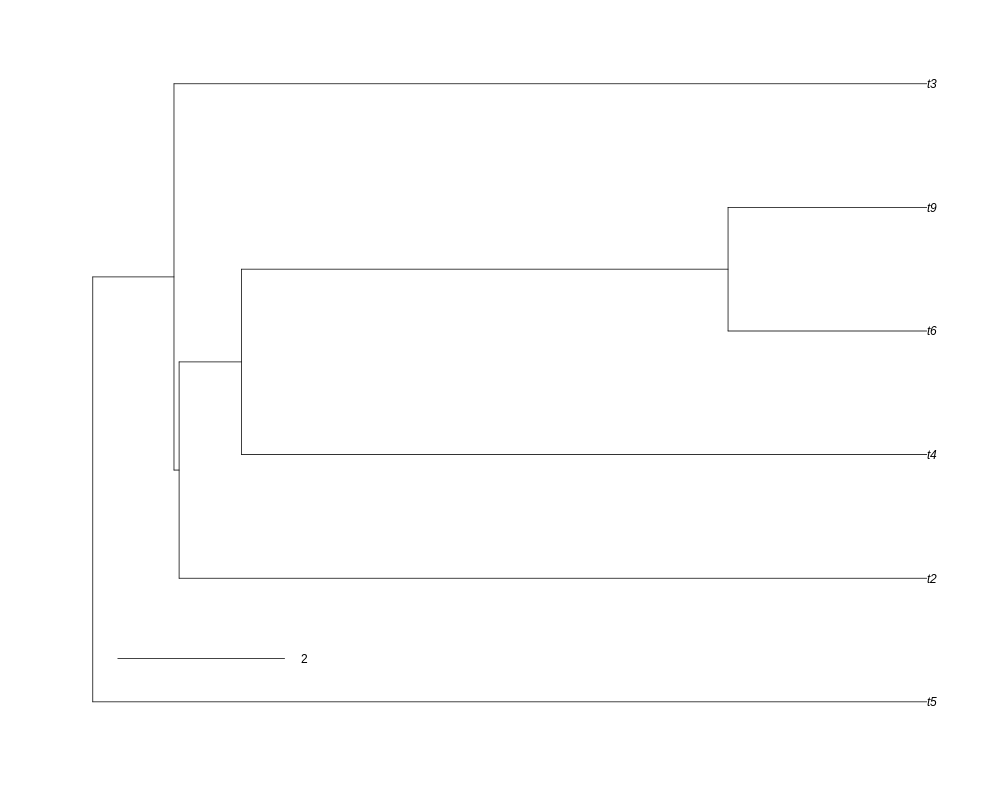
\includegraphics[height=0.4\textheight]{pirouette_example_30/example_30_314/true_tree.png}
    };   
    \node[state] (B) [below of = A, rectangle] {
      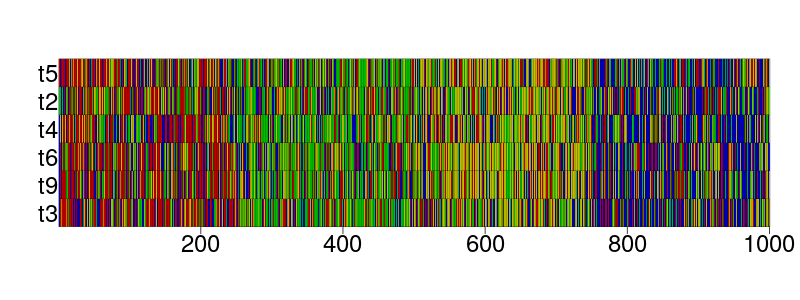
\includegraphics[height=0.25\textheight]{pirouette_example_30/example_30_314/true_alignment.png}
    };   
    \node[state] (CG) [below of = B, rectangle] {
      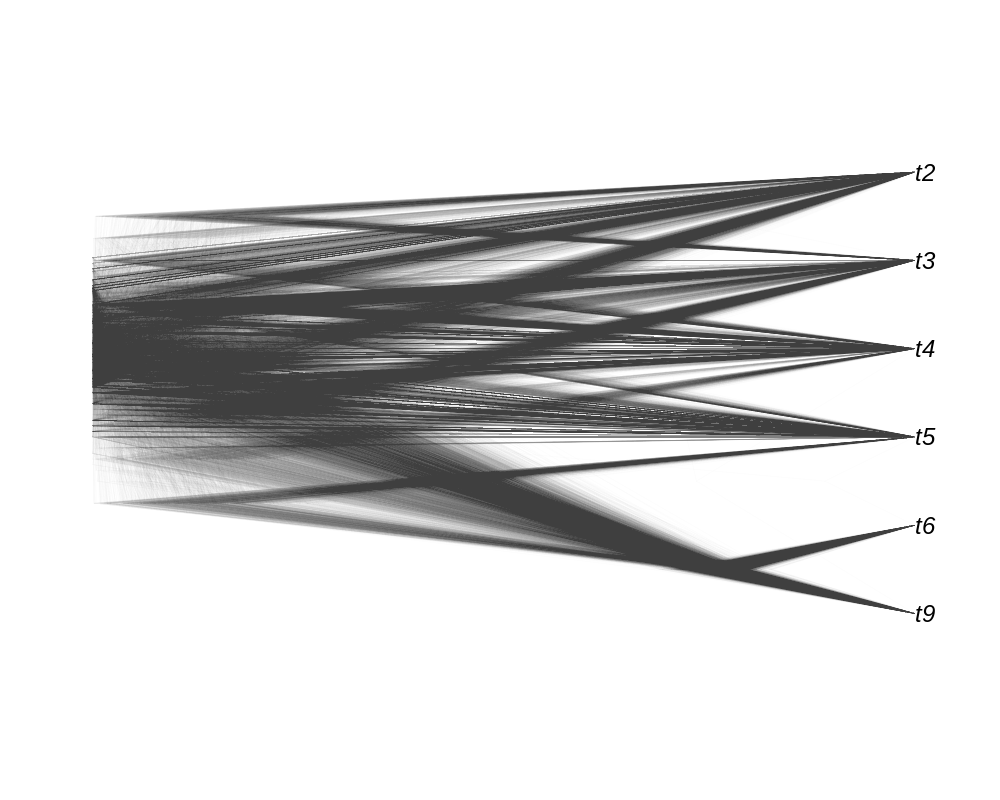
\includegraphics[height=0.3\textheight]{pirouette_example_30/example_30_314/true_posterior_gen.png}
    };   
    \node[state] (DG) [below of = CG, rectangle] {
      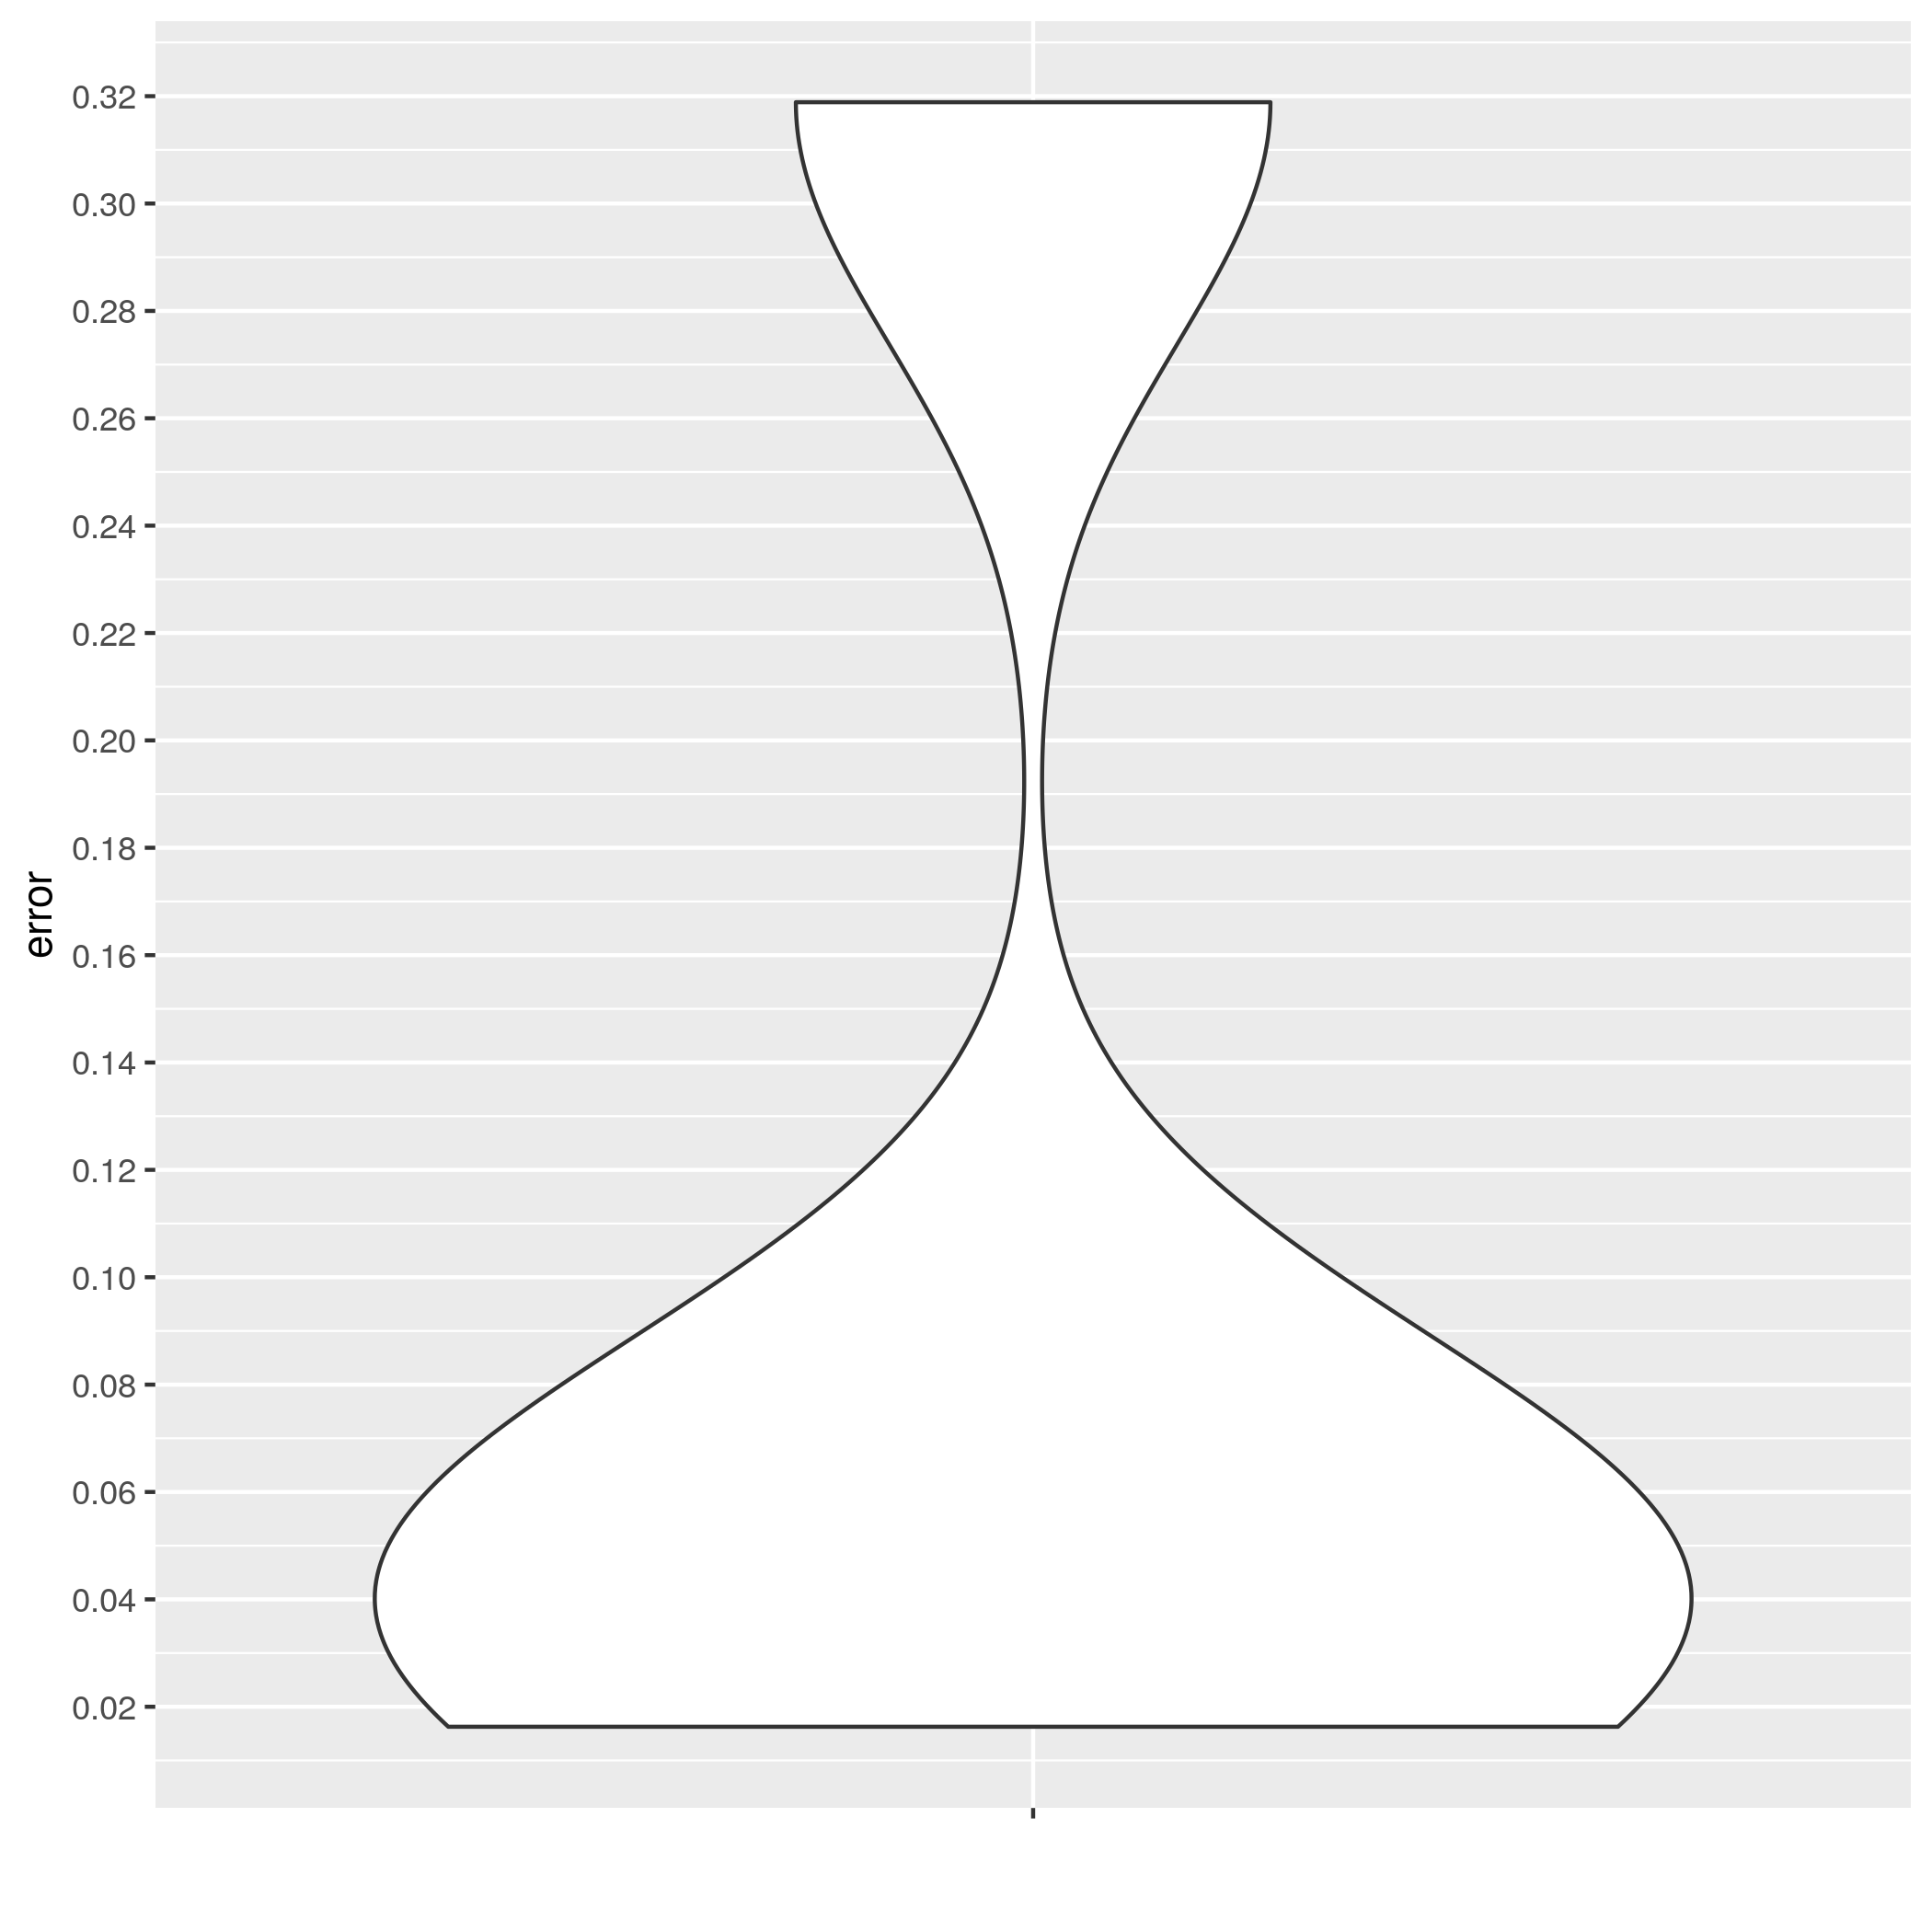
\includegraphics[height=0.3\textheight]{pirouette_example_30/example_30_314/true_error_violin_gen.png}
    };   
    \node[state] (CB) [right of = CG, rectangle] {
      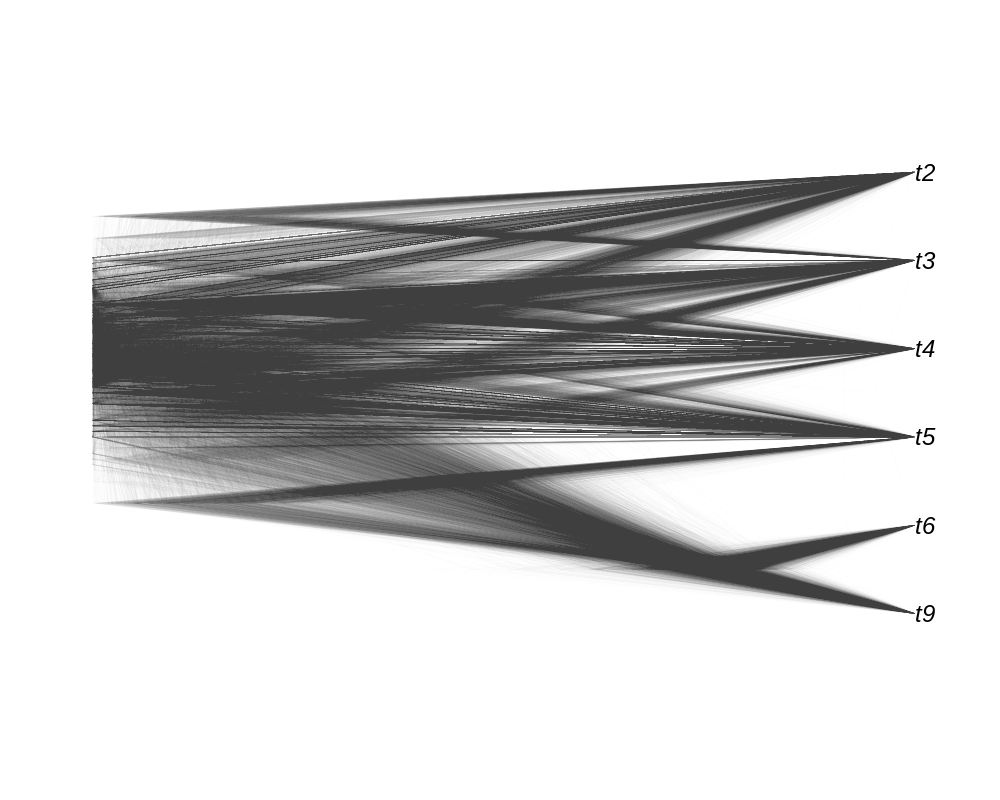
\includegraphics[height=0.3\textheight]{pirouette_example_30/example_30_314/true_posterior_best.png}
    };   
    \node[state] (DB) [below of = CB, rectangle] {
      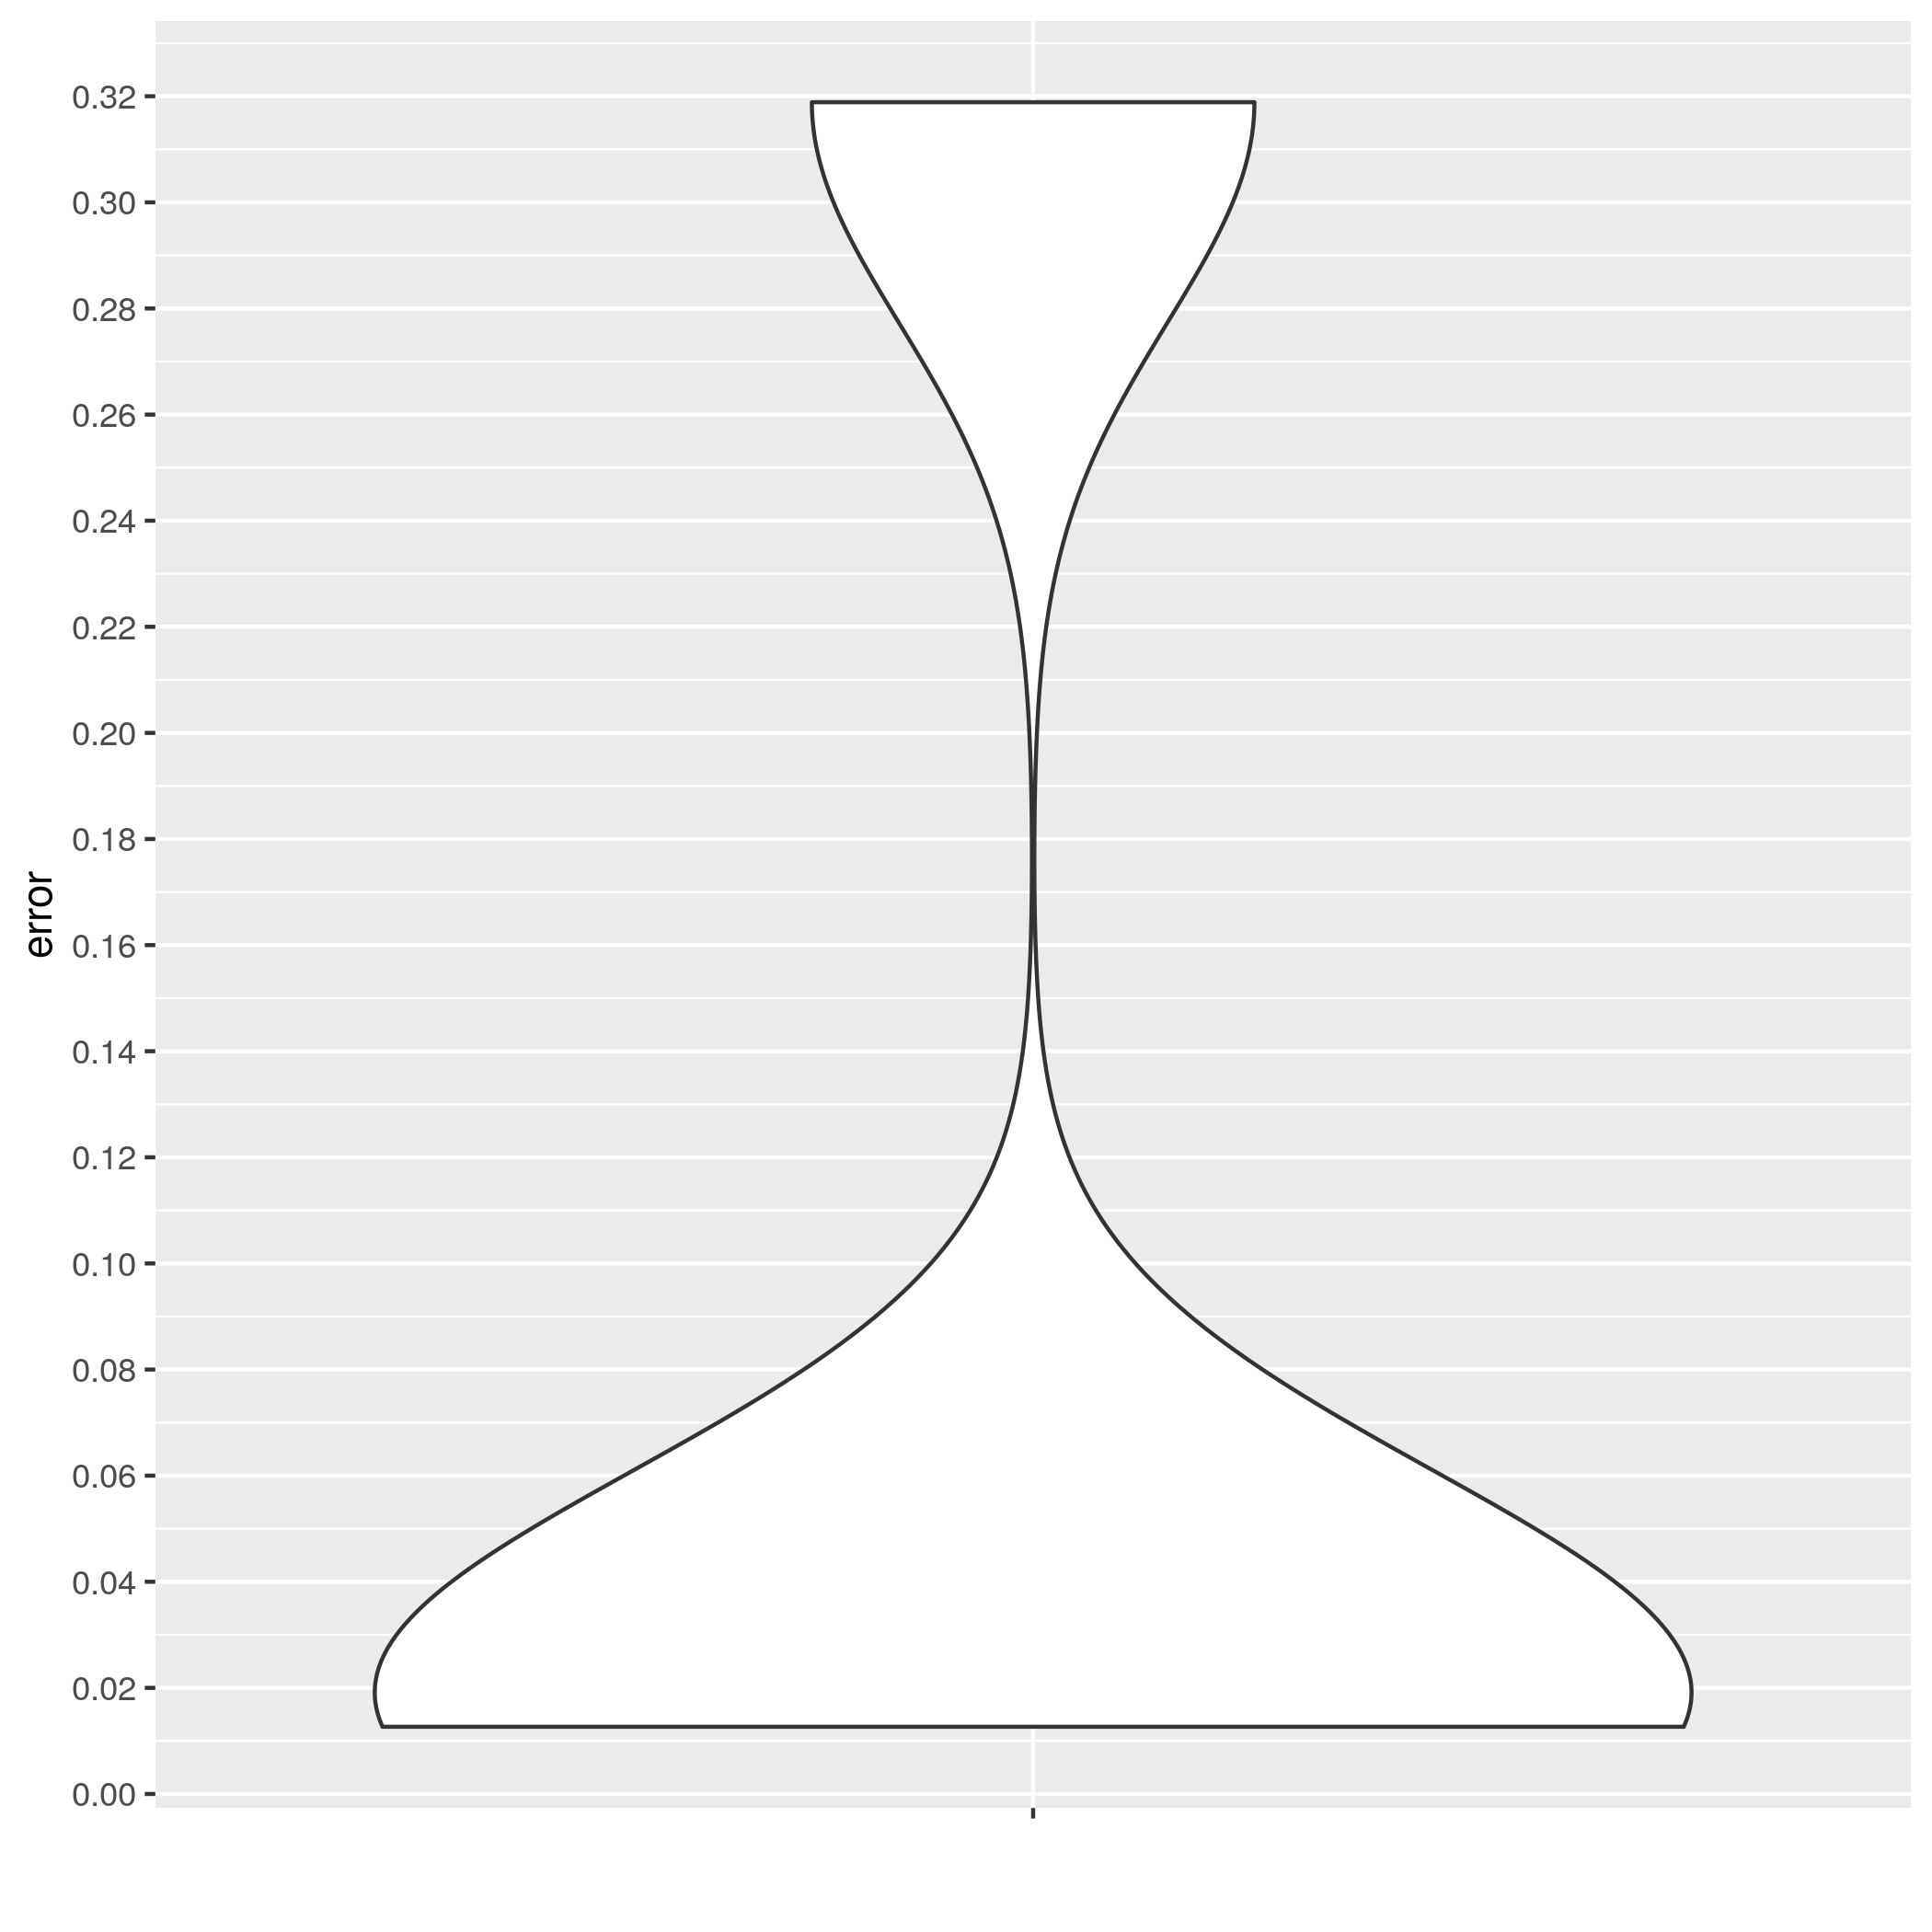
\includegraphics[height=0.3\textheight]{pirouette_example_30/example_30_314/true_error_violin_best.png}
    };   
    \node[state] (AT) [right of = A, rectangle, node distance=0.8\textheight] {
      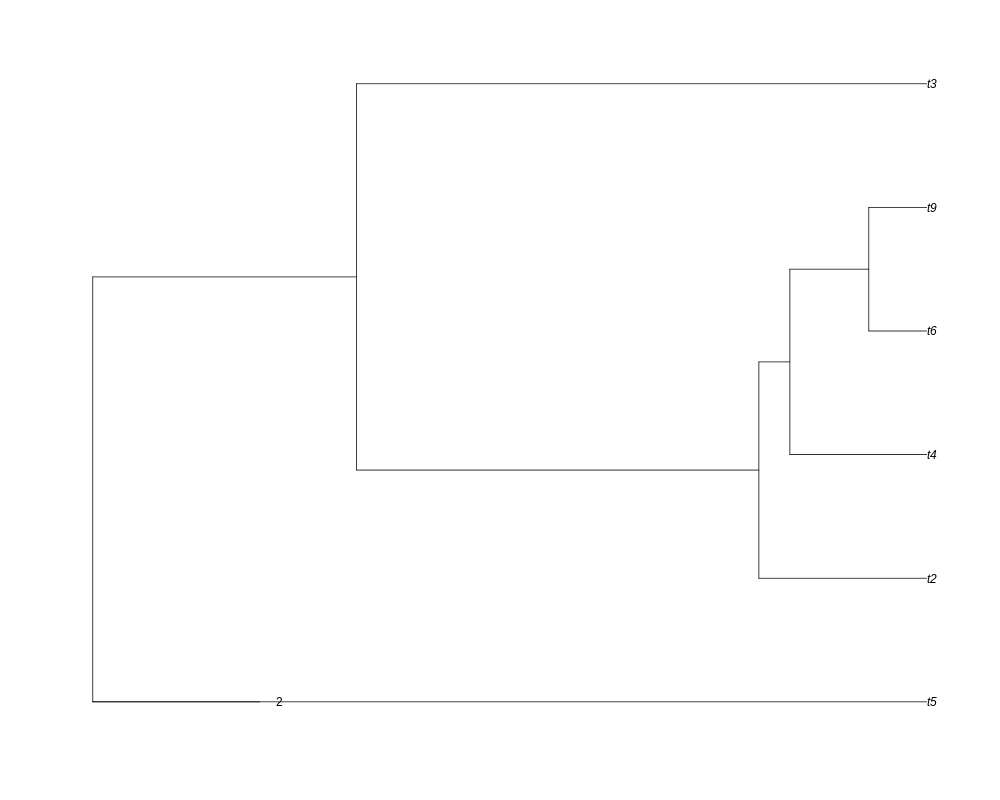
\includegraphics[height=0.4\textheight]{pirouette_example_30/example_30_314/twin_tree.png}
    };   
    \node[state] (BT) [below of = AT, rectangle] {
      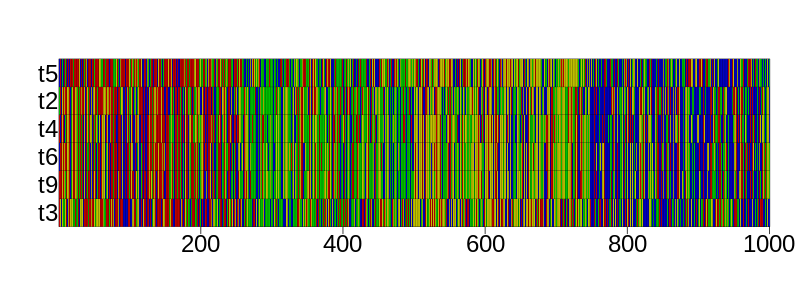
\includegraphics[height=0.25\textheight]{pirouette_example_30/example_30_314/twin_alignment.png}
    };   
    \node[state] (CTG) [right of = CB, rectangle] {
      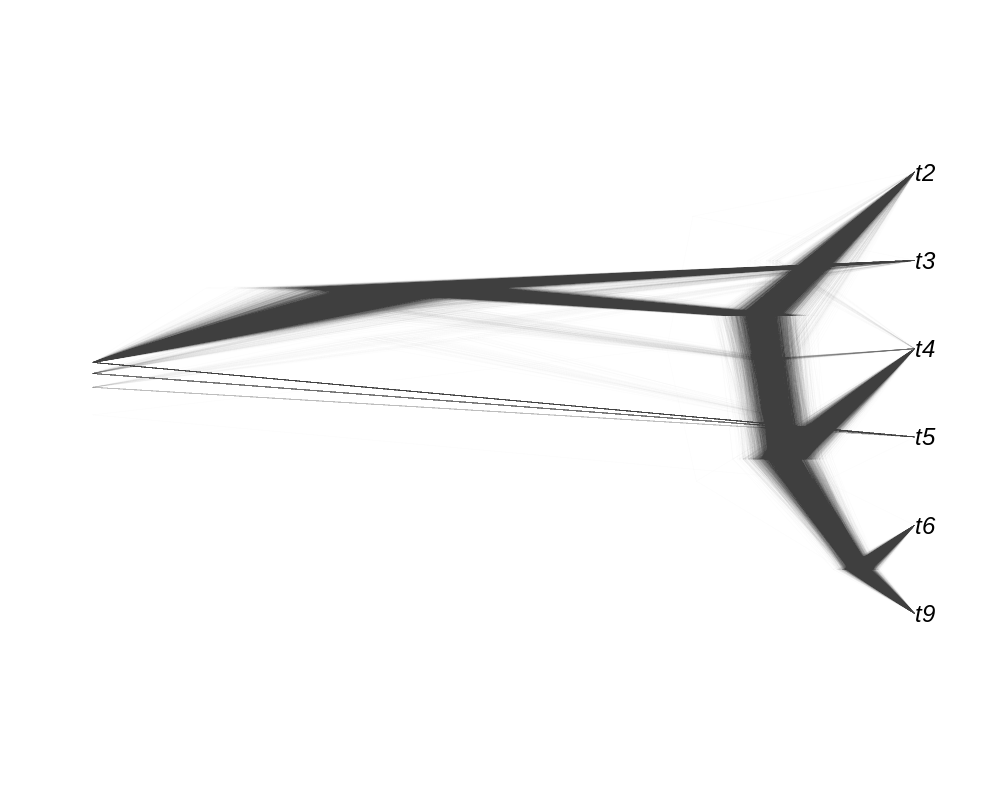
\includegraphics[height=0.3\textheight]{pirouette_example_30/example_30_314/twin_posterior_gen.png}
    };   
    \node[state] (DTG) [below of = CTG, rectangle] {
      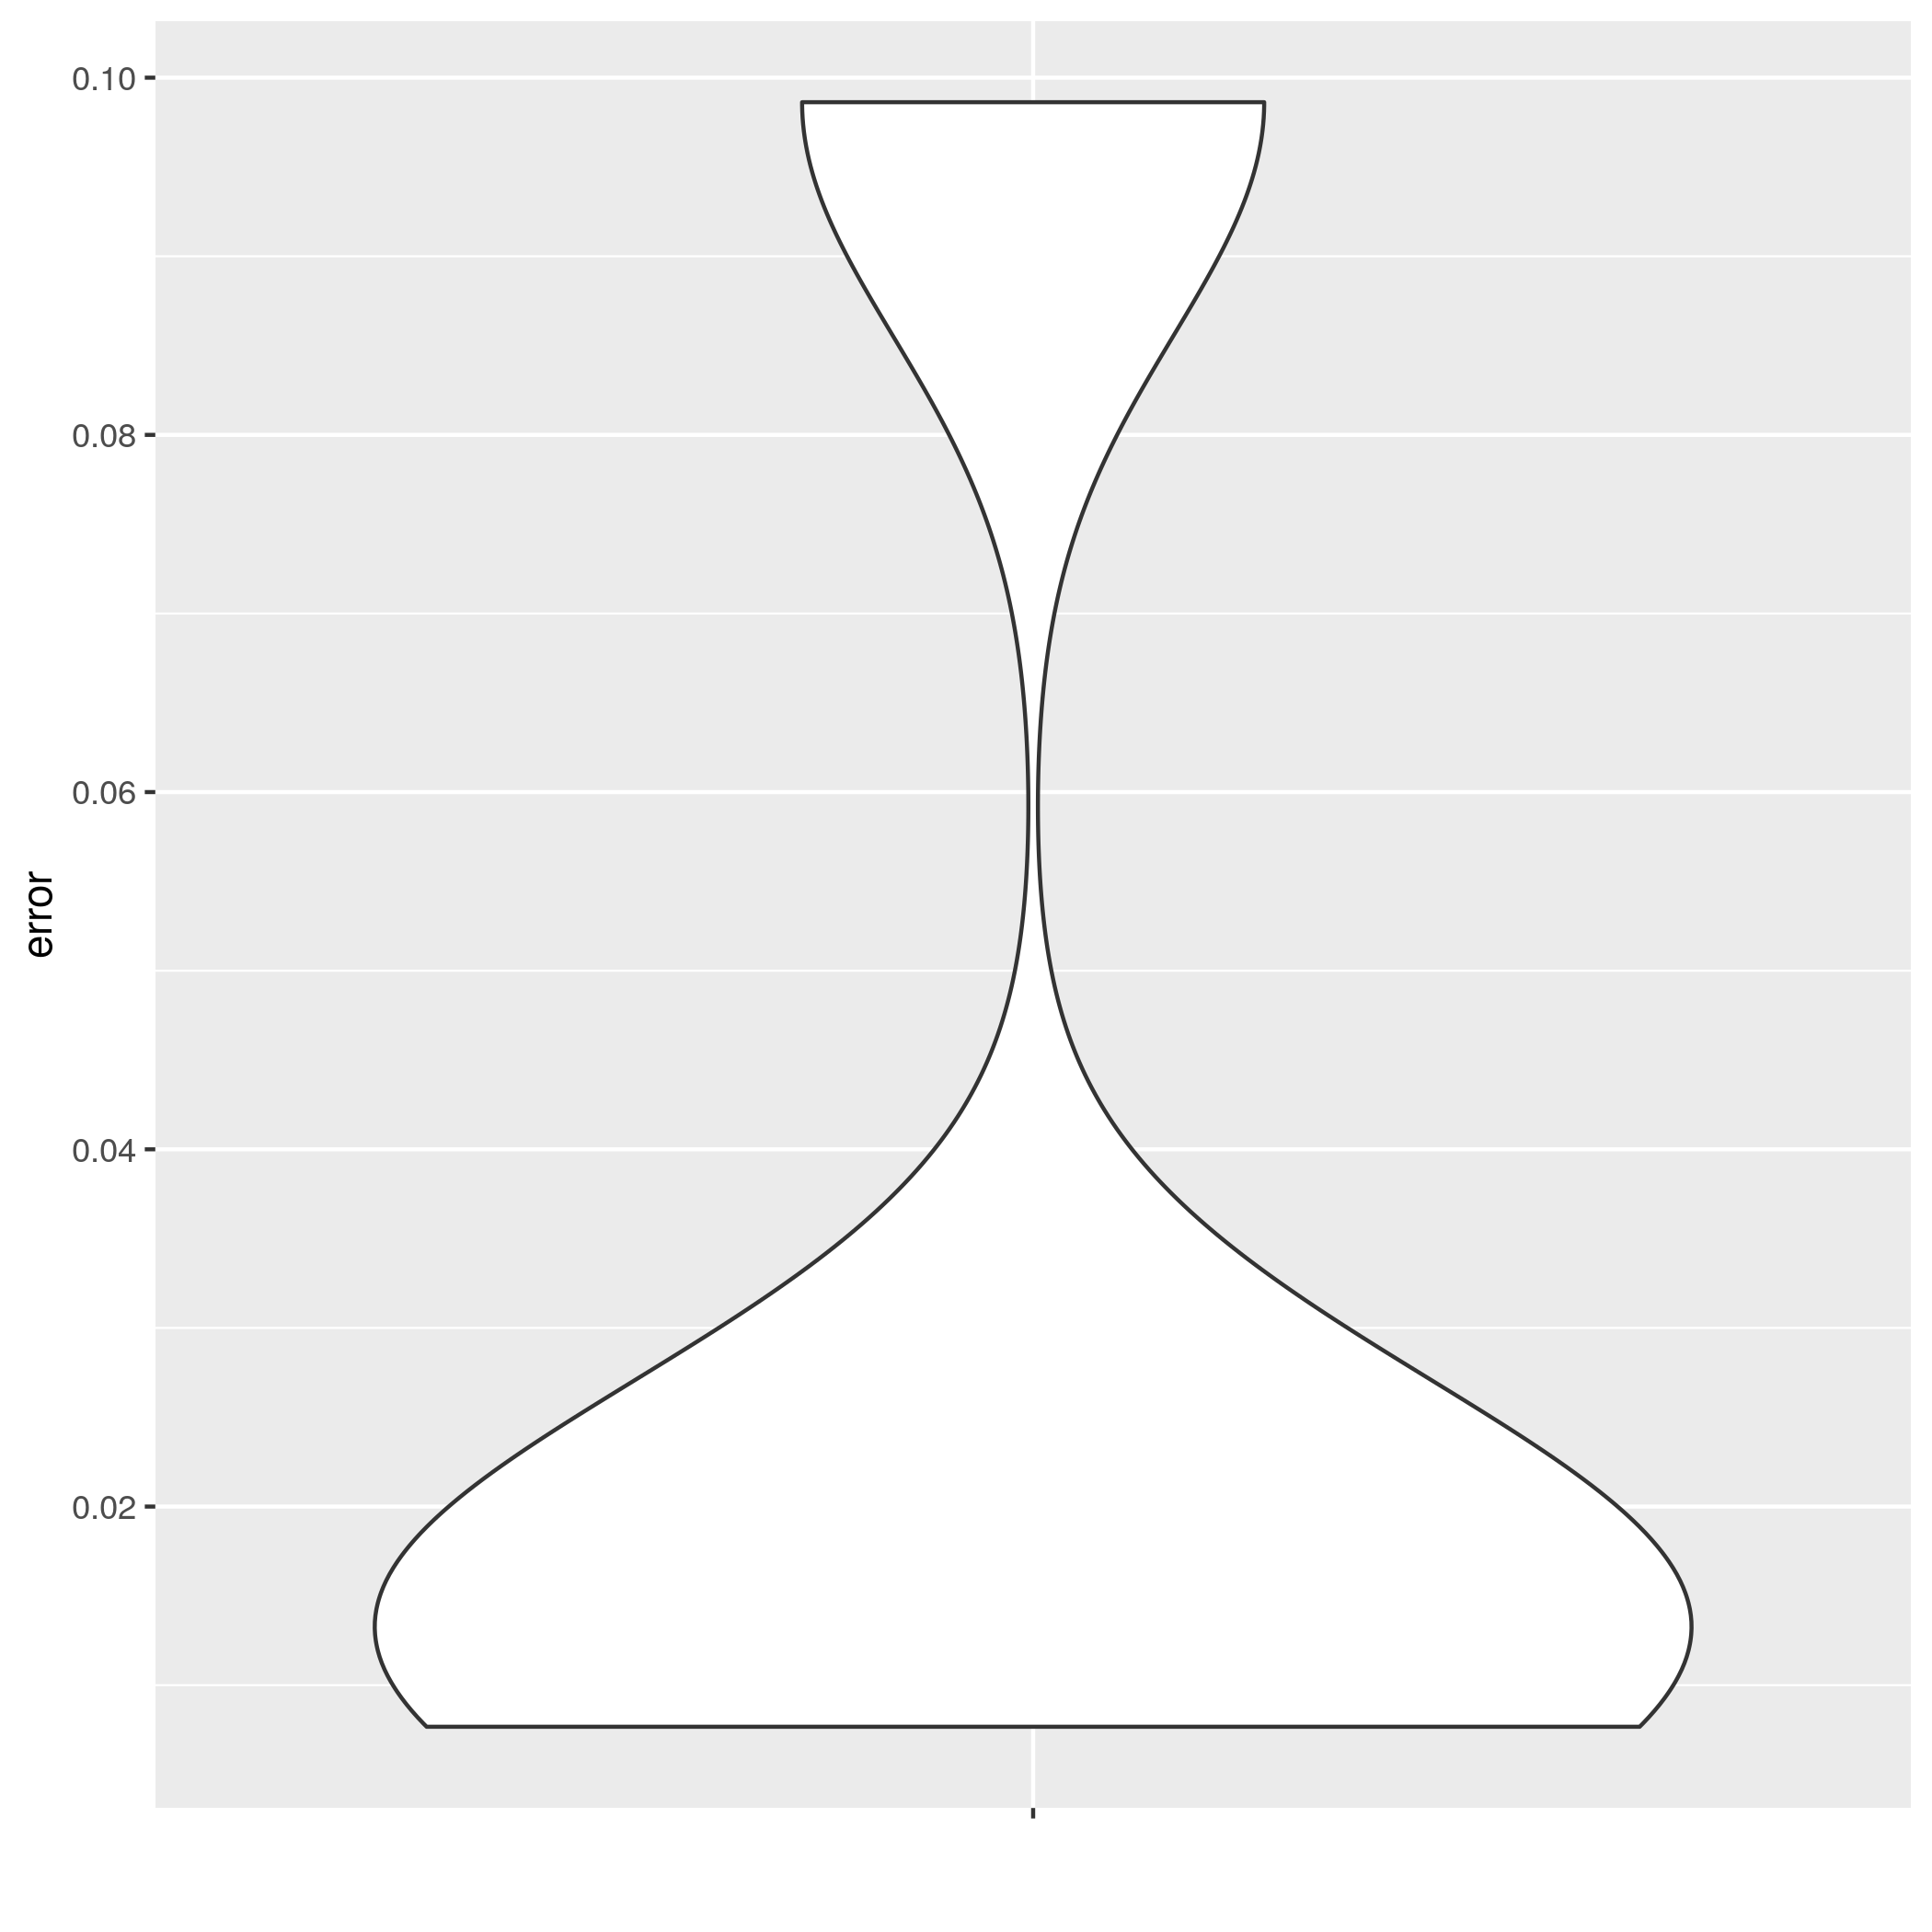
\includegraphics[height=0.3\textheight]{pirouette_example_30/example_30_314/twin_error_violin_gen.png}
    };   
    \node[state] (CTB) [right of = CTG, rectangle] {
      
\includegraphics[height=0.3\textheight]{pirouette_example_30/example_30_314/twin_posterior_best.png}
    };   
    \node[state] (DTB) [below of = CTB, rectangle] {
      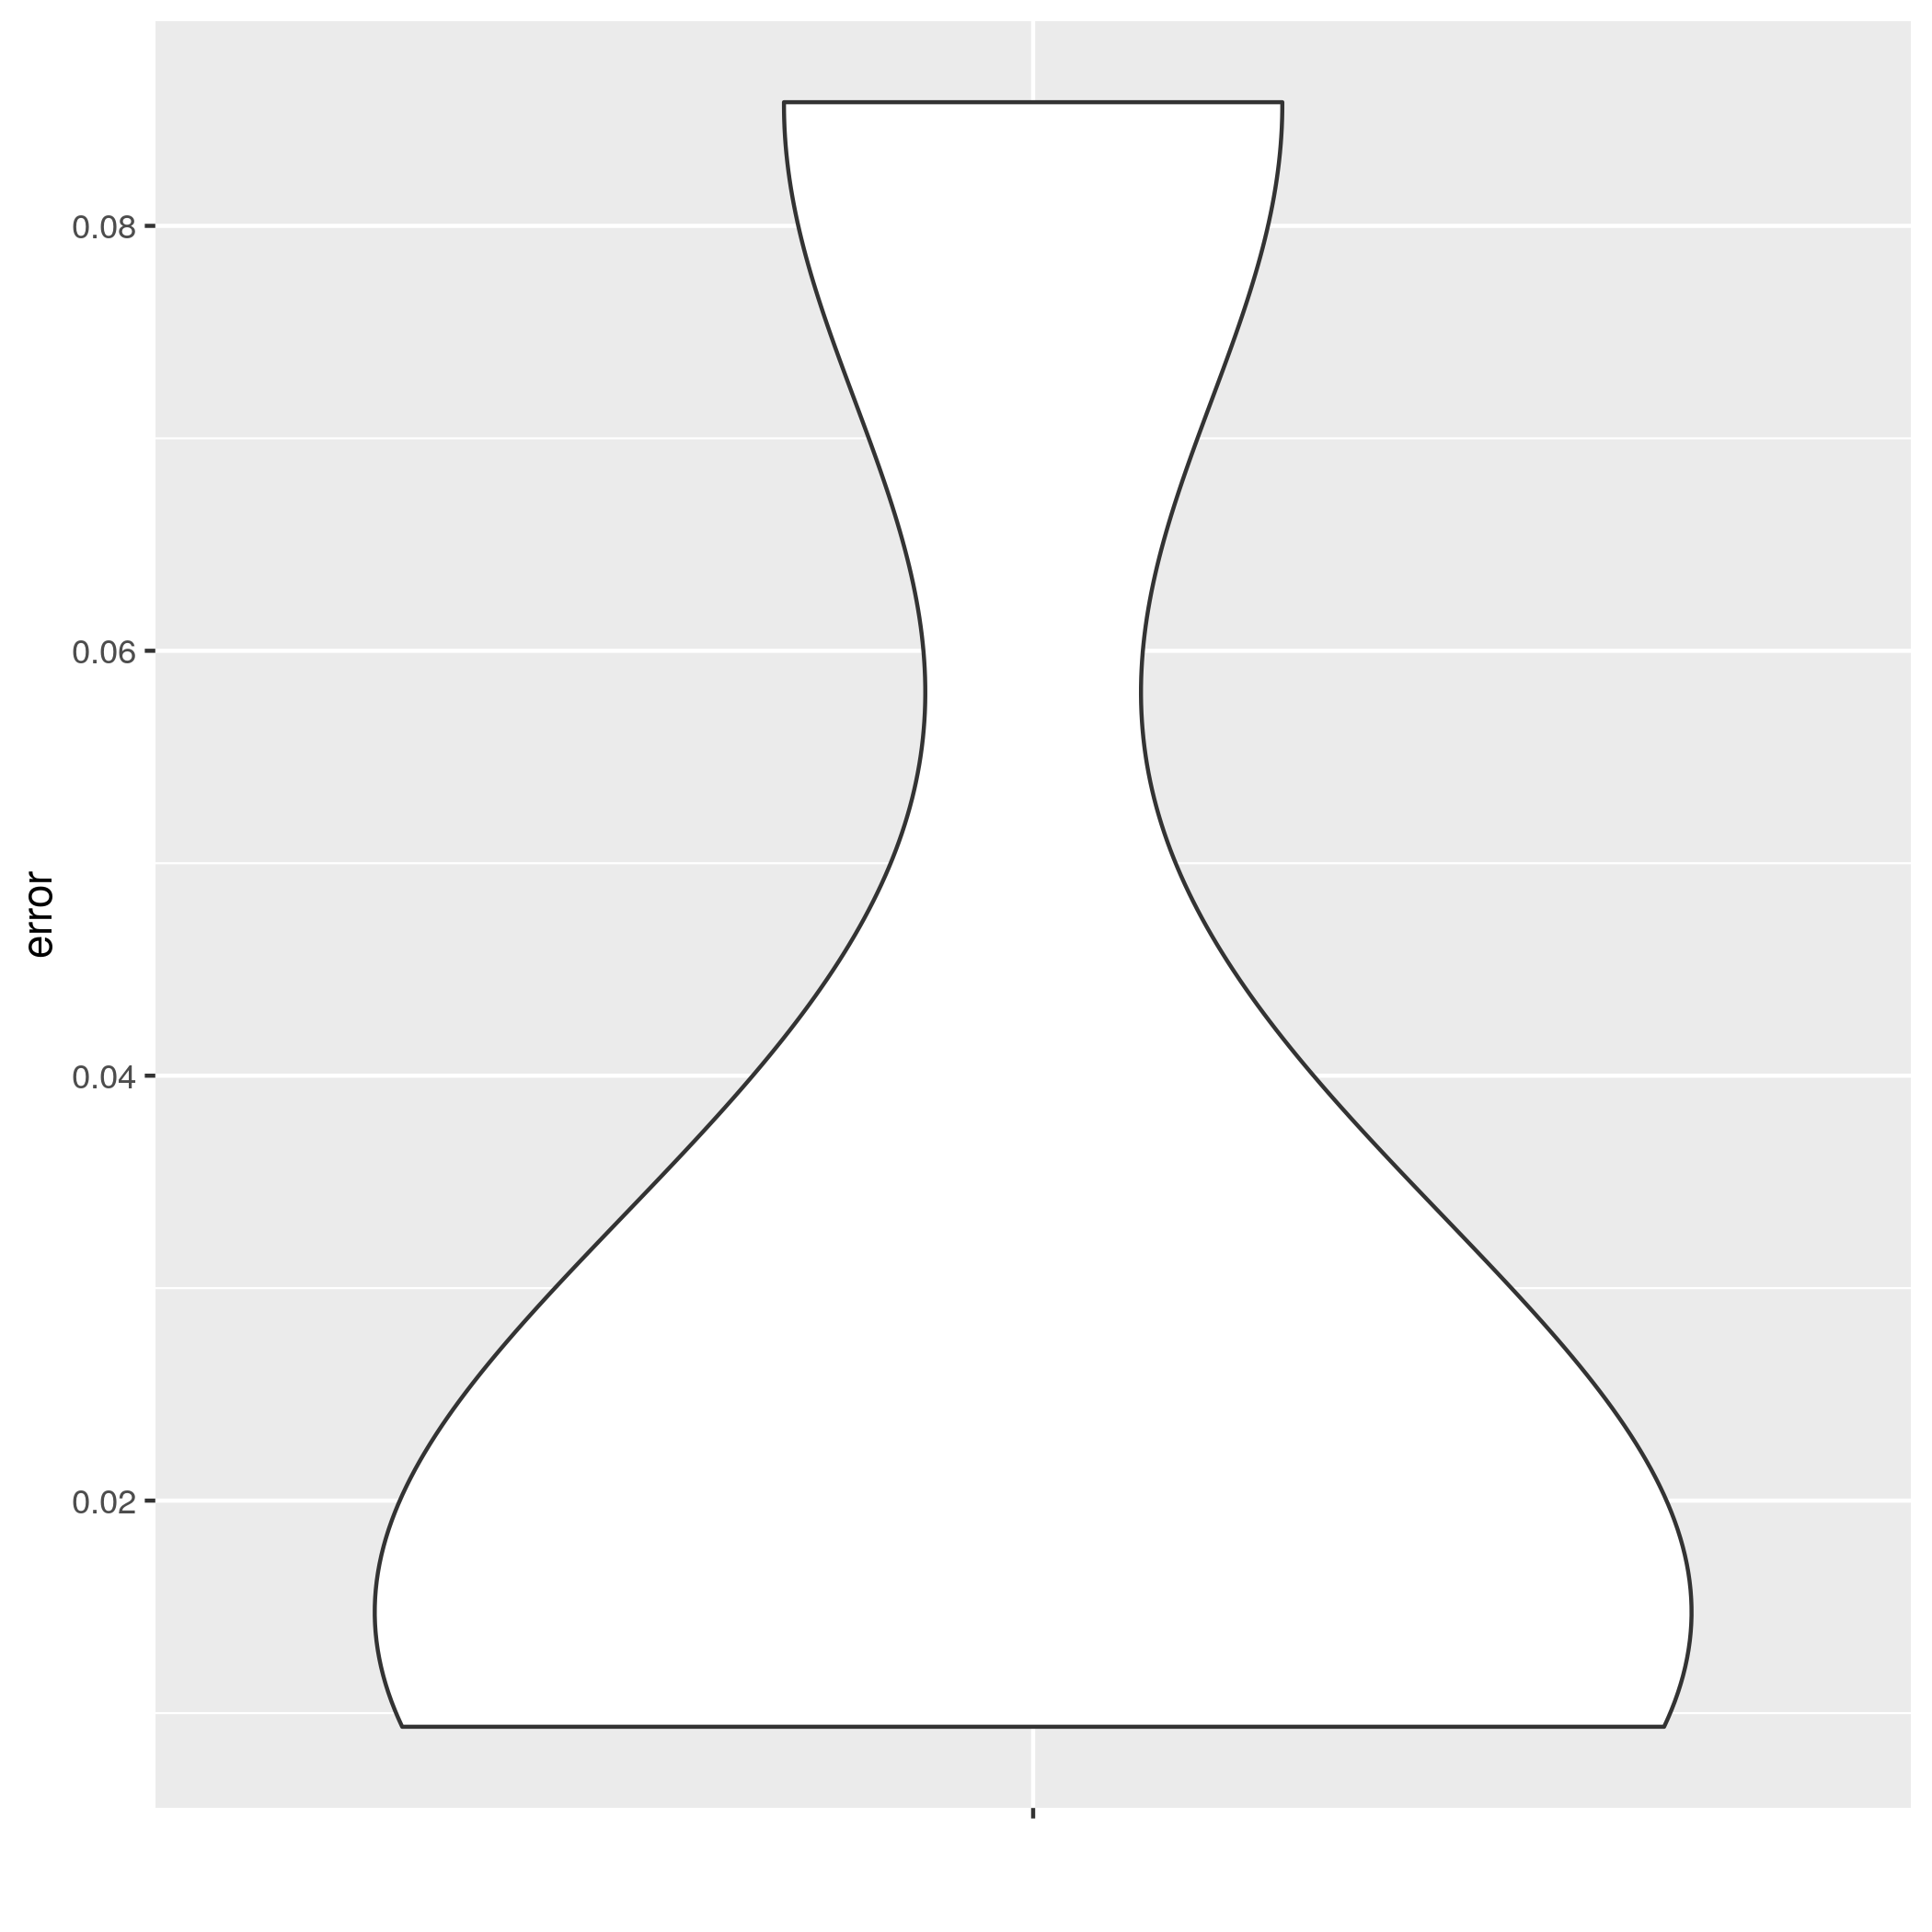
\includegraphics[height=0.3\textheight]{pirouette_example_30/example_30_314/twin_error_violin_best.png}
    };   
    \path 
      (O) edge [anchor = south] node {} (A)
      (A) edge [anchor = south] node {} (B)
      (B) edge [anchor = south] node {} (CG)
      (CG) edge [anchor = south] node {} (DG)
      (B) edge [anchor = south east] node {} (CB)
      (CB) edge [anchor = south] node {} (DB)
      (A) edge [anchor = east] node {} (AT)
      (AT) edge [anchor = south] node {} (BT)
      (BT) edge [anchor = south east] node {} (CTG)
      (CTG) edge [anchor = south] node {} (DTG)
      (BT) edge [anchor = south] node {} (CTB)
      (CTB) edge [anchor = south] node {} (DTB)
    ; 
    \end{tikzpicture}
  }
  \label{fig:example_30_full_pipeline}
  \caption{Comparing to background noise: full pipeline}
\end{figure}
%%%%%%%%%%%%%%%%%%%%%%%%%%%%%%%%%%%%%%%%%%%%%%%%%%%%%%%%%%%%%%%%%%%%%%%%%%%%%%%%

\input{pirouette_example_30/example_30_314/esses_gen.latex}

\input{pirouette_example_30/example_30_314/esses_best.latex}

\input{pirouette_example_30/example_30_314/esses_twin_gen.latex}

\input{pirouette_example_30/example_30_314/esses_twin_best.latex}

\input{pirouette_example_30/example_30_314/evidence_true.latex}

\input{pirouette_example_30/example_30_314/evidence_twin.latex}

%%%%%%%%%%%%%%%%%%%%%%%%%%%%%%%%%%%%%%%%%%%%%%%%%%%%%%%%%%%%%%%%%%%%%%%%%%%%%%%%
\subsection{Using a distribution of trees}
\label{subsec:distribution}
%%%%%%%%%%%%%%%%%%%%%%%%%%%%%%%%%%%%%%%%%%%%%%%%%%%%%%%%%%%%%%%%%%%%%%%%%%%%%%%%

\richel{Issue \url{https://github.com/richelbilderbeek/pirouette_article/issues/89}}

This subsection extends the main example, by using multiple (instead of
one) trees. These trees are produced by running a DD tree simulation
with the same parameters as the main example, which are
speciation rate \richel{?}, extinction rate $0.1$, and carrying
capacity 40. 

The code used in this part of the article can be found at 
\url{https://github.com/richelbilderbeek/pirouette_example_28}.

\begin{figure}[H]
  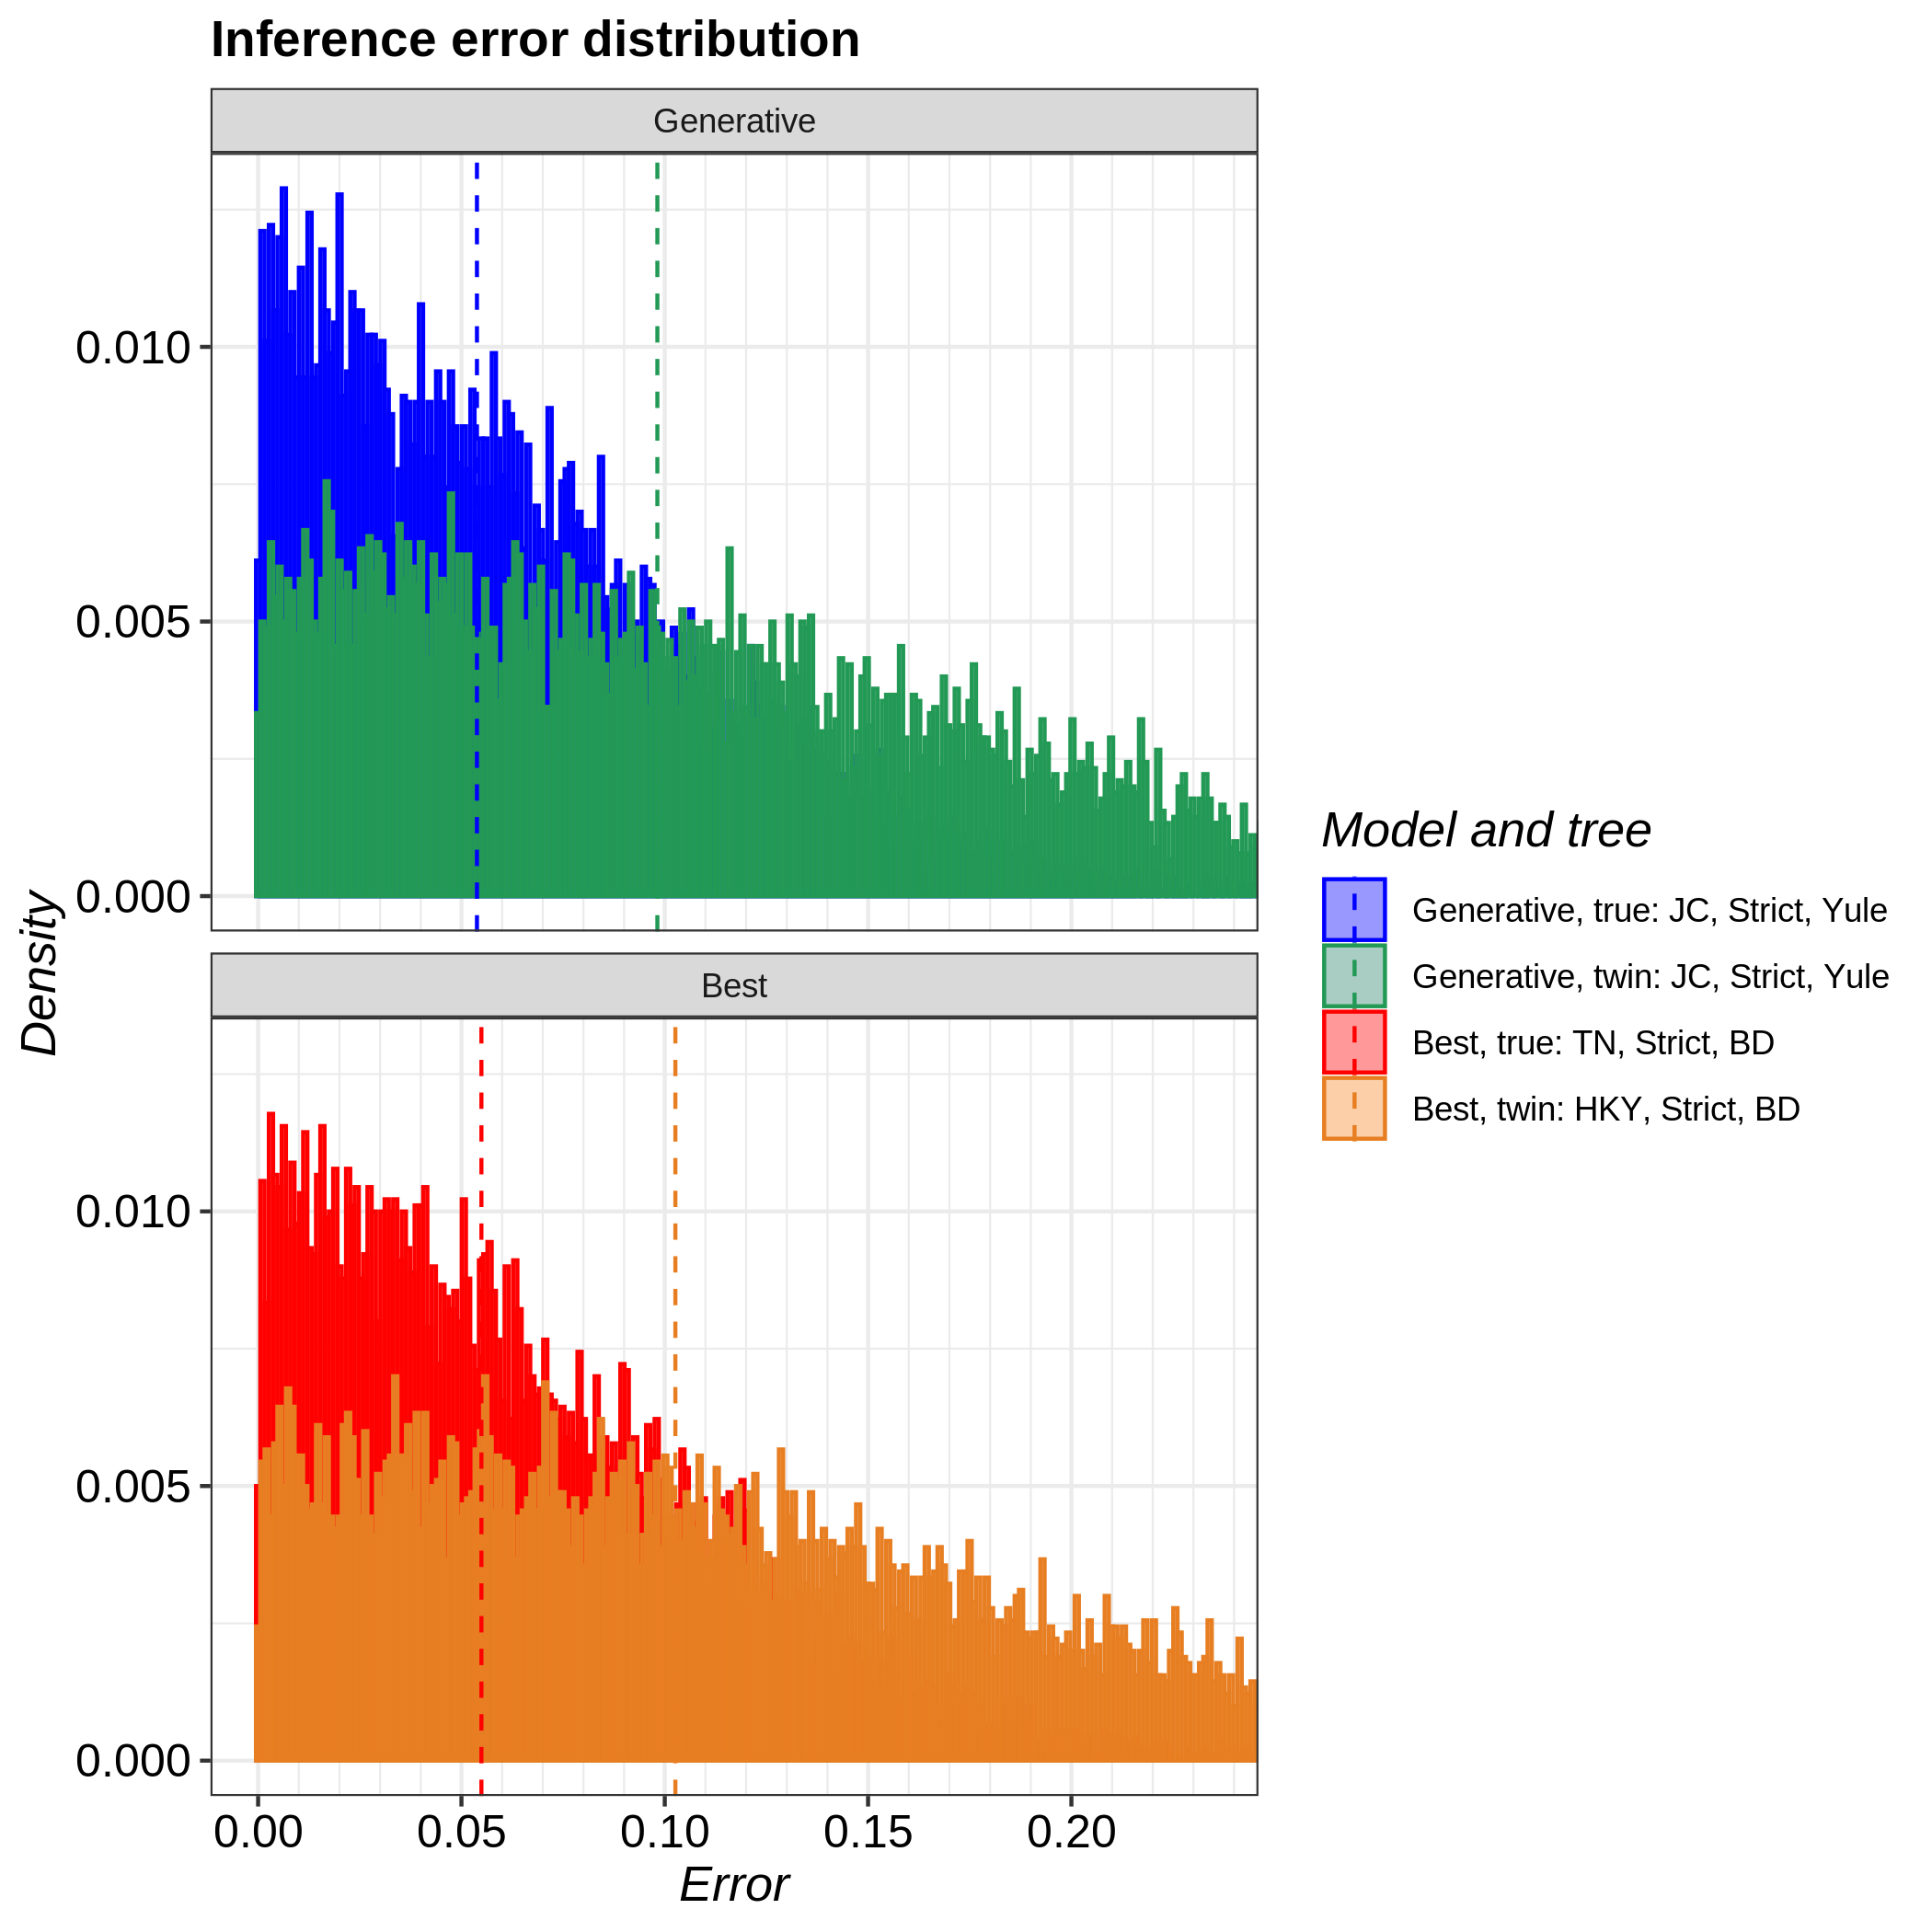
\includegraphics[width=\textwidth]{pirouette_example_28/example_28_314/errors.png}
  \caption{Error distribution from a distribution of trees}
\end{figure}

%%%%%%%%%%%%%%%%%%%%%%%%%%%%%%%%%%%%%%%%%%%%%%%%%%%%%%%%%%%%%%%%%%%%%%%%%%%%%%%%
\subsection{The effect of the number of taxa}
%%%%%%%%%%%%%%%%%%%%%%%%%%%%%%%%%%%%%%%%%%%%%%%%%%%%%%%%%%%%%%%%%%%%%%%%%%%%%%%%

The code used in this part of the article can be found at 
\url{https://github.com/richelbilderbeek/pirouette_example_20}. 

\begin{figure}[H]
  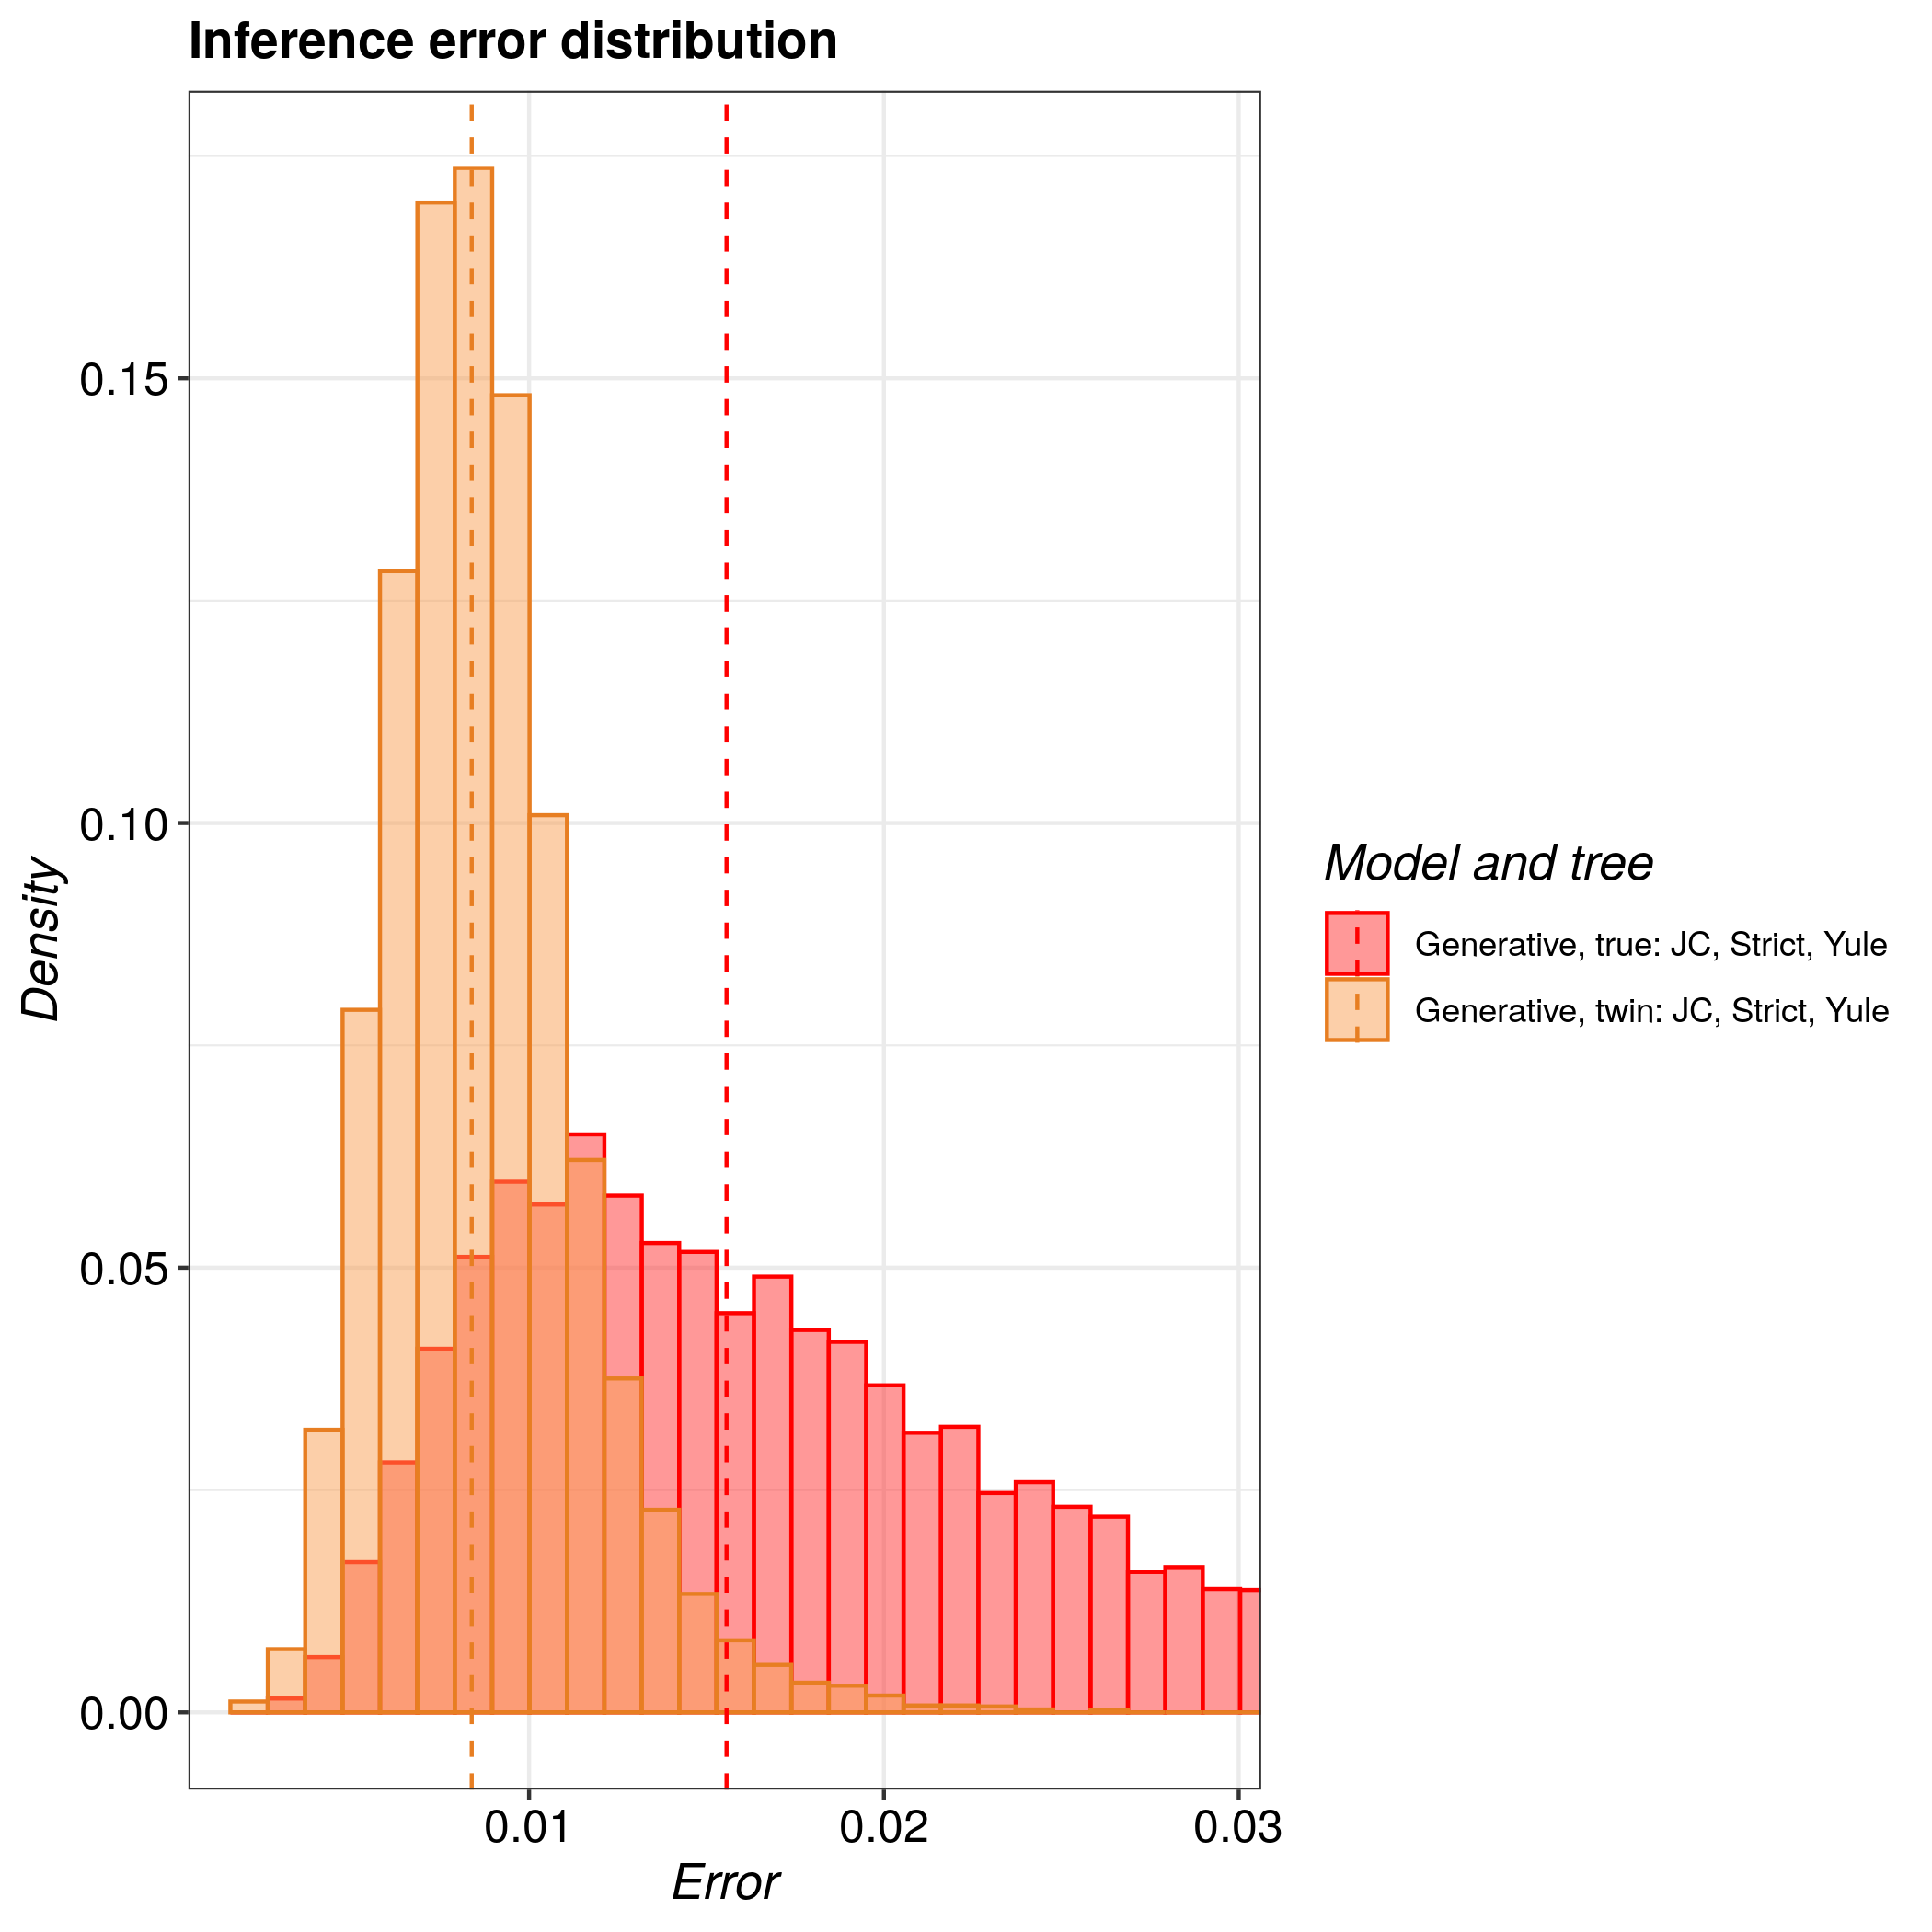
\includegraphics[width=\textwidth]{pirouette_example_20/example_20_314/errors.png}
  \caption{10 taxa}
\end{figure}

\begin{figure}[H]
  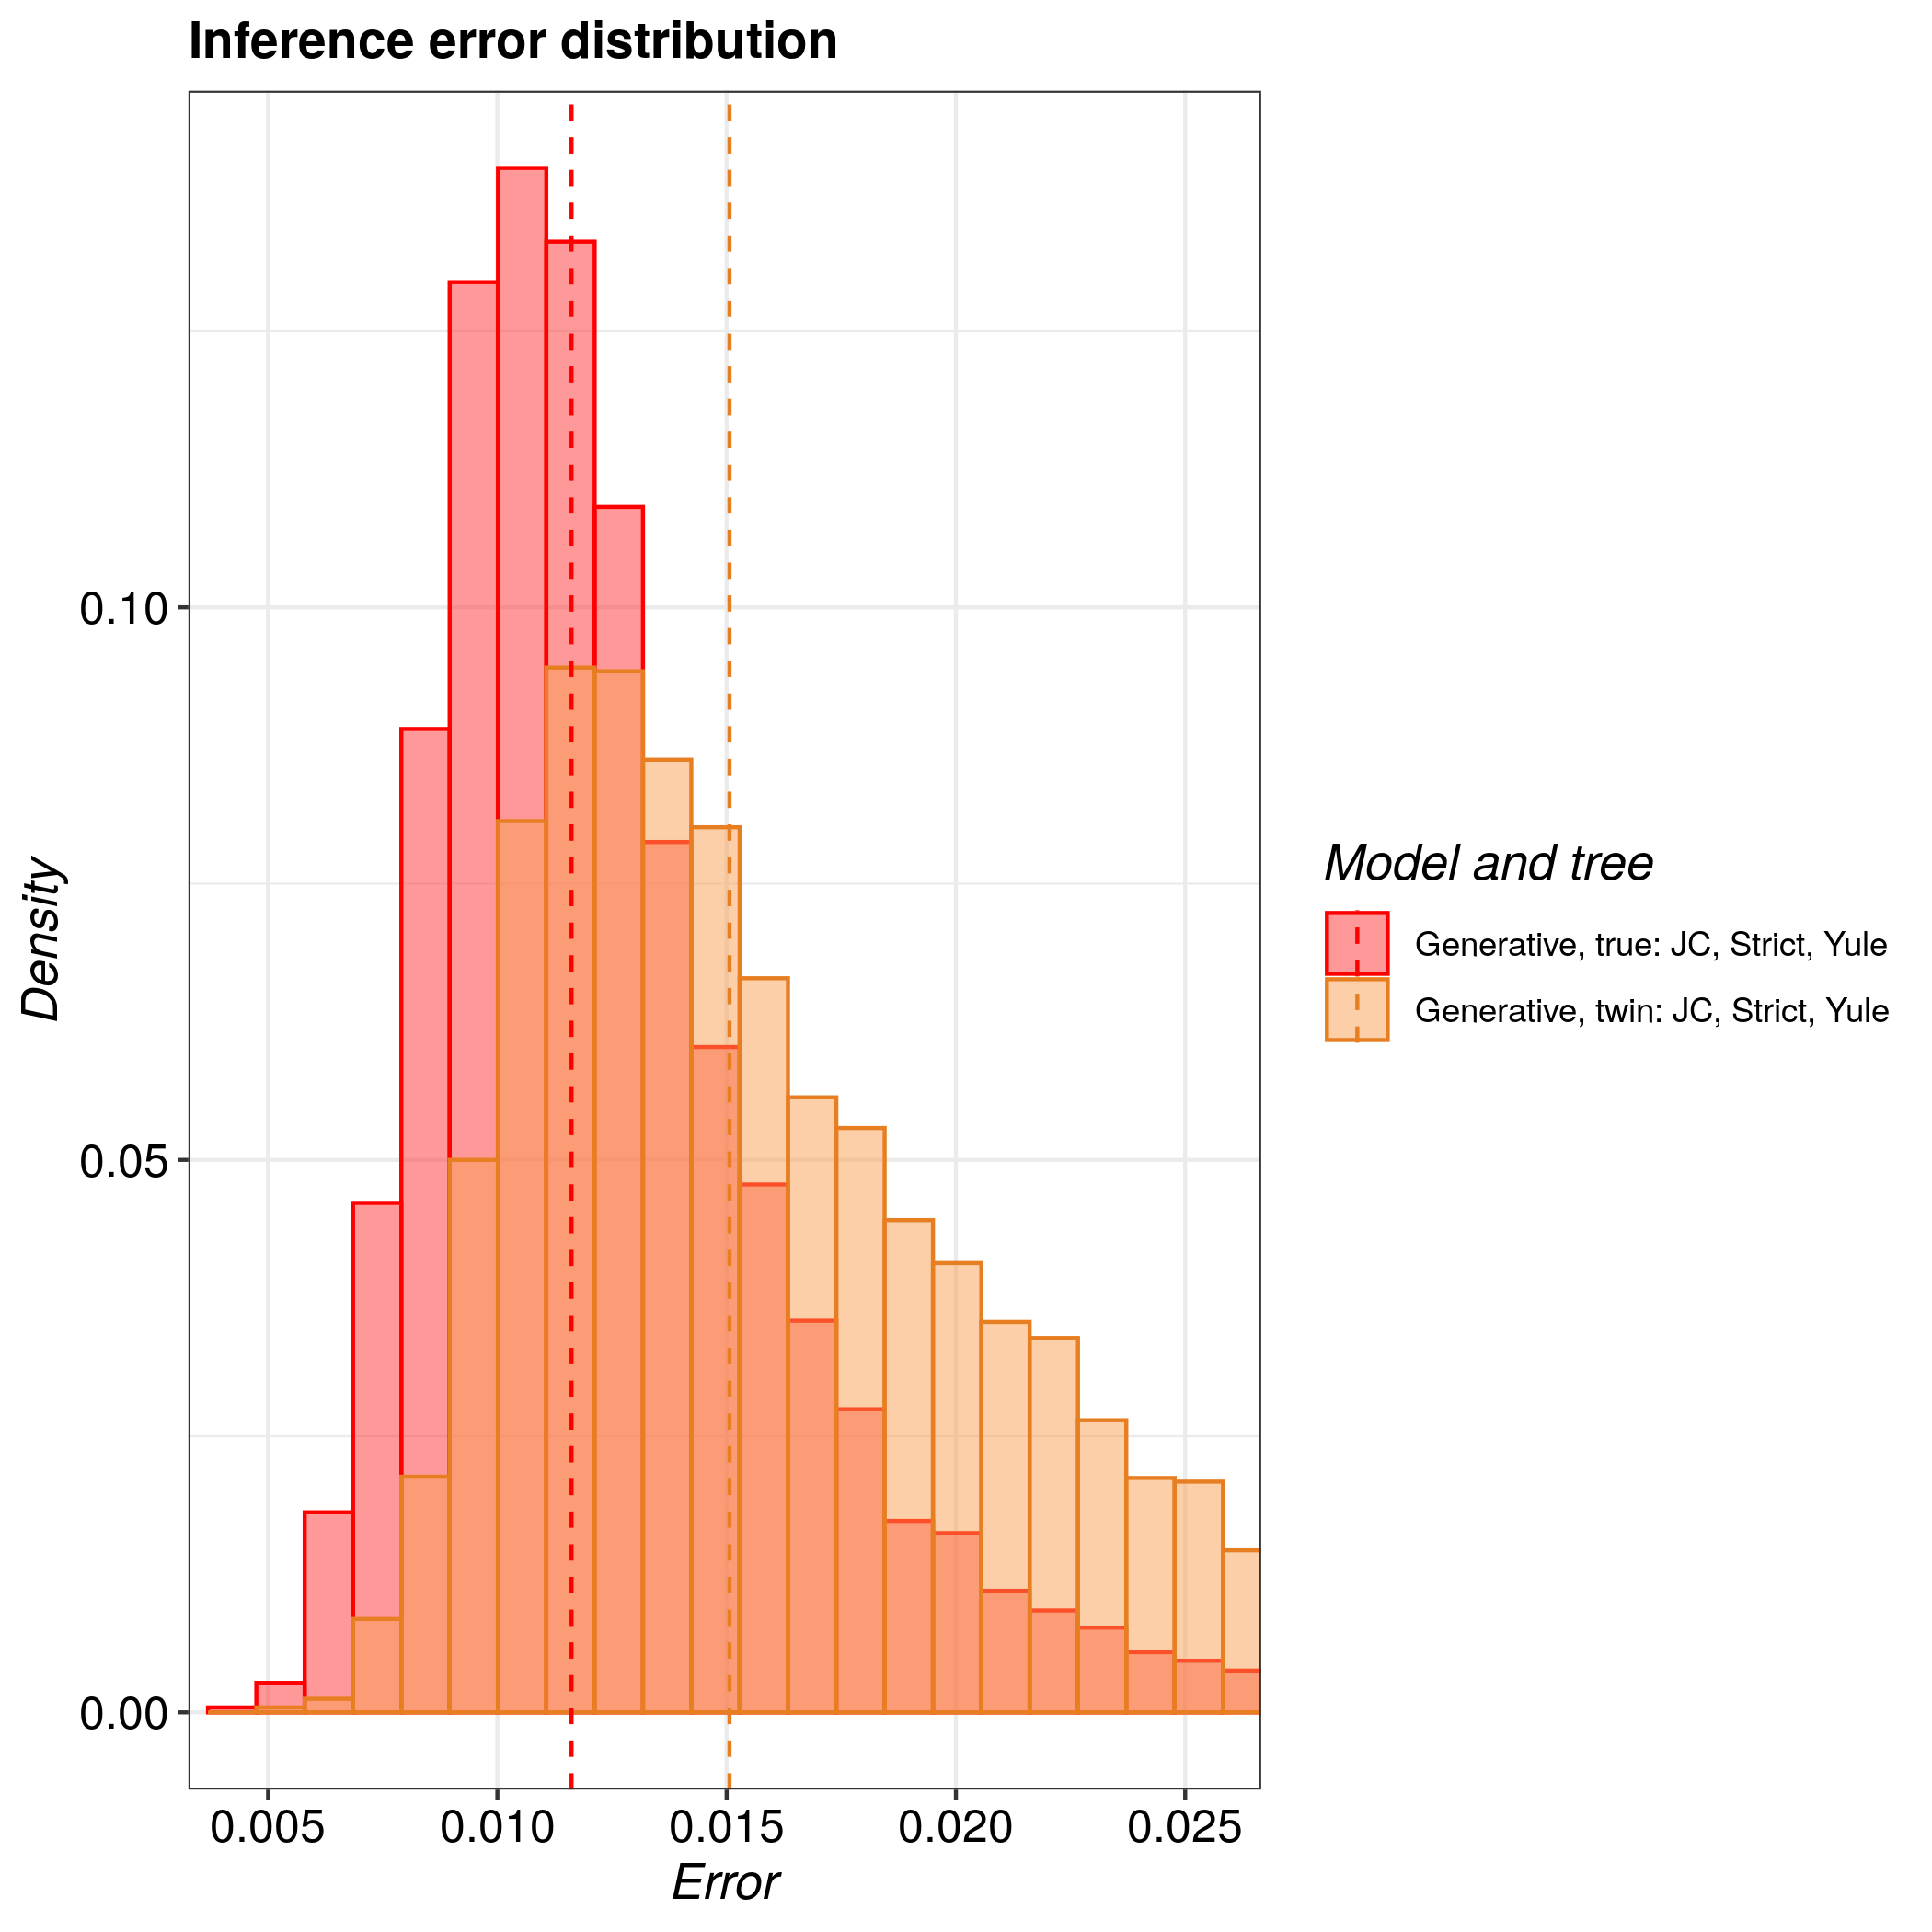
\includegraphics[width=\textwidth]{pirouette_example_20/example_20_315/errors.png}
  \caption{20 taxa}
\end{figure}

\begin{figure}[H]
  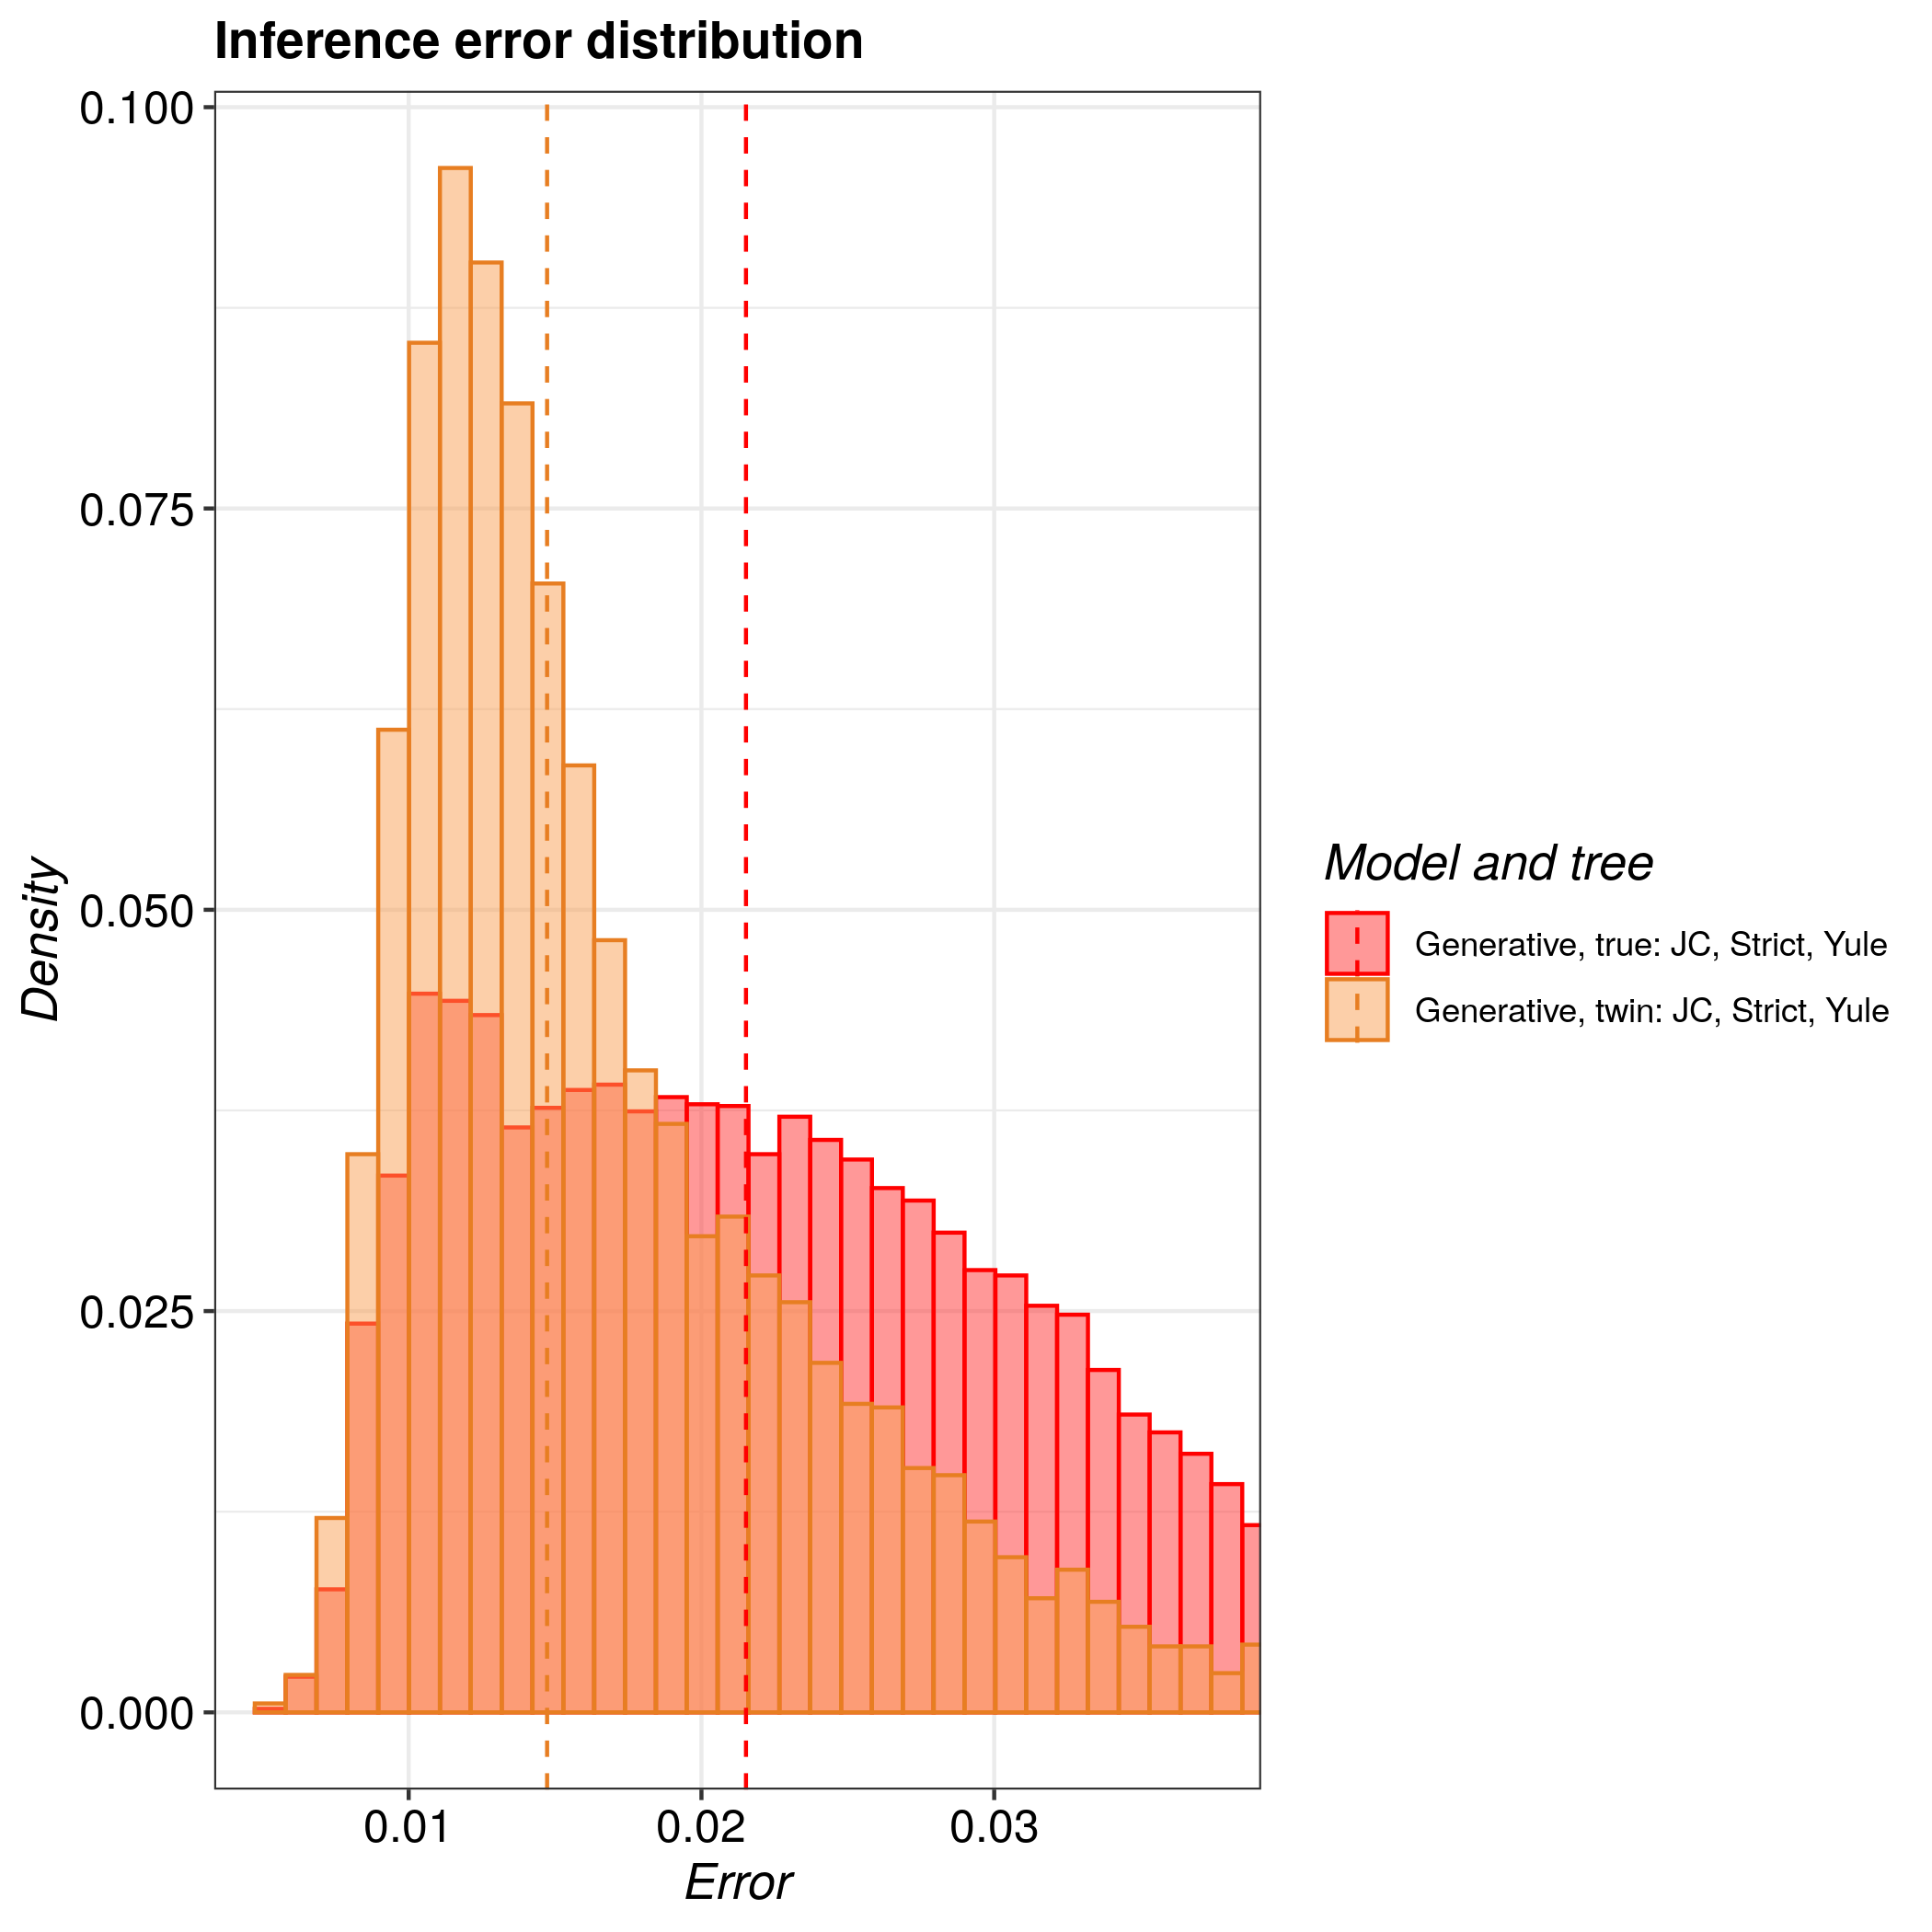
\includegraphics[width=\textwidth]{pirouette_example_20/example_20_316/errors.png}
  \caption{30 taxa}
\end{figure}

\begin{figure}[H]
  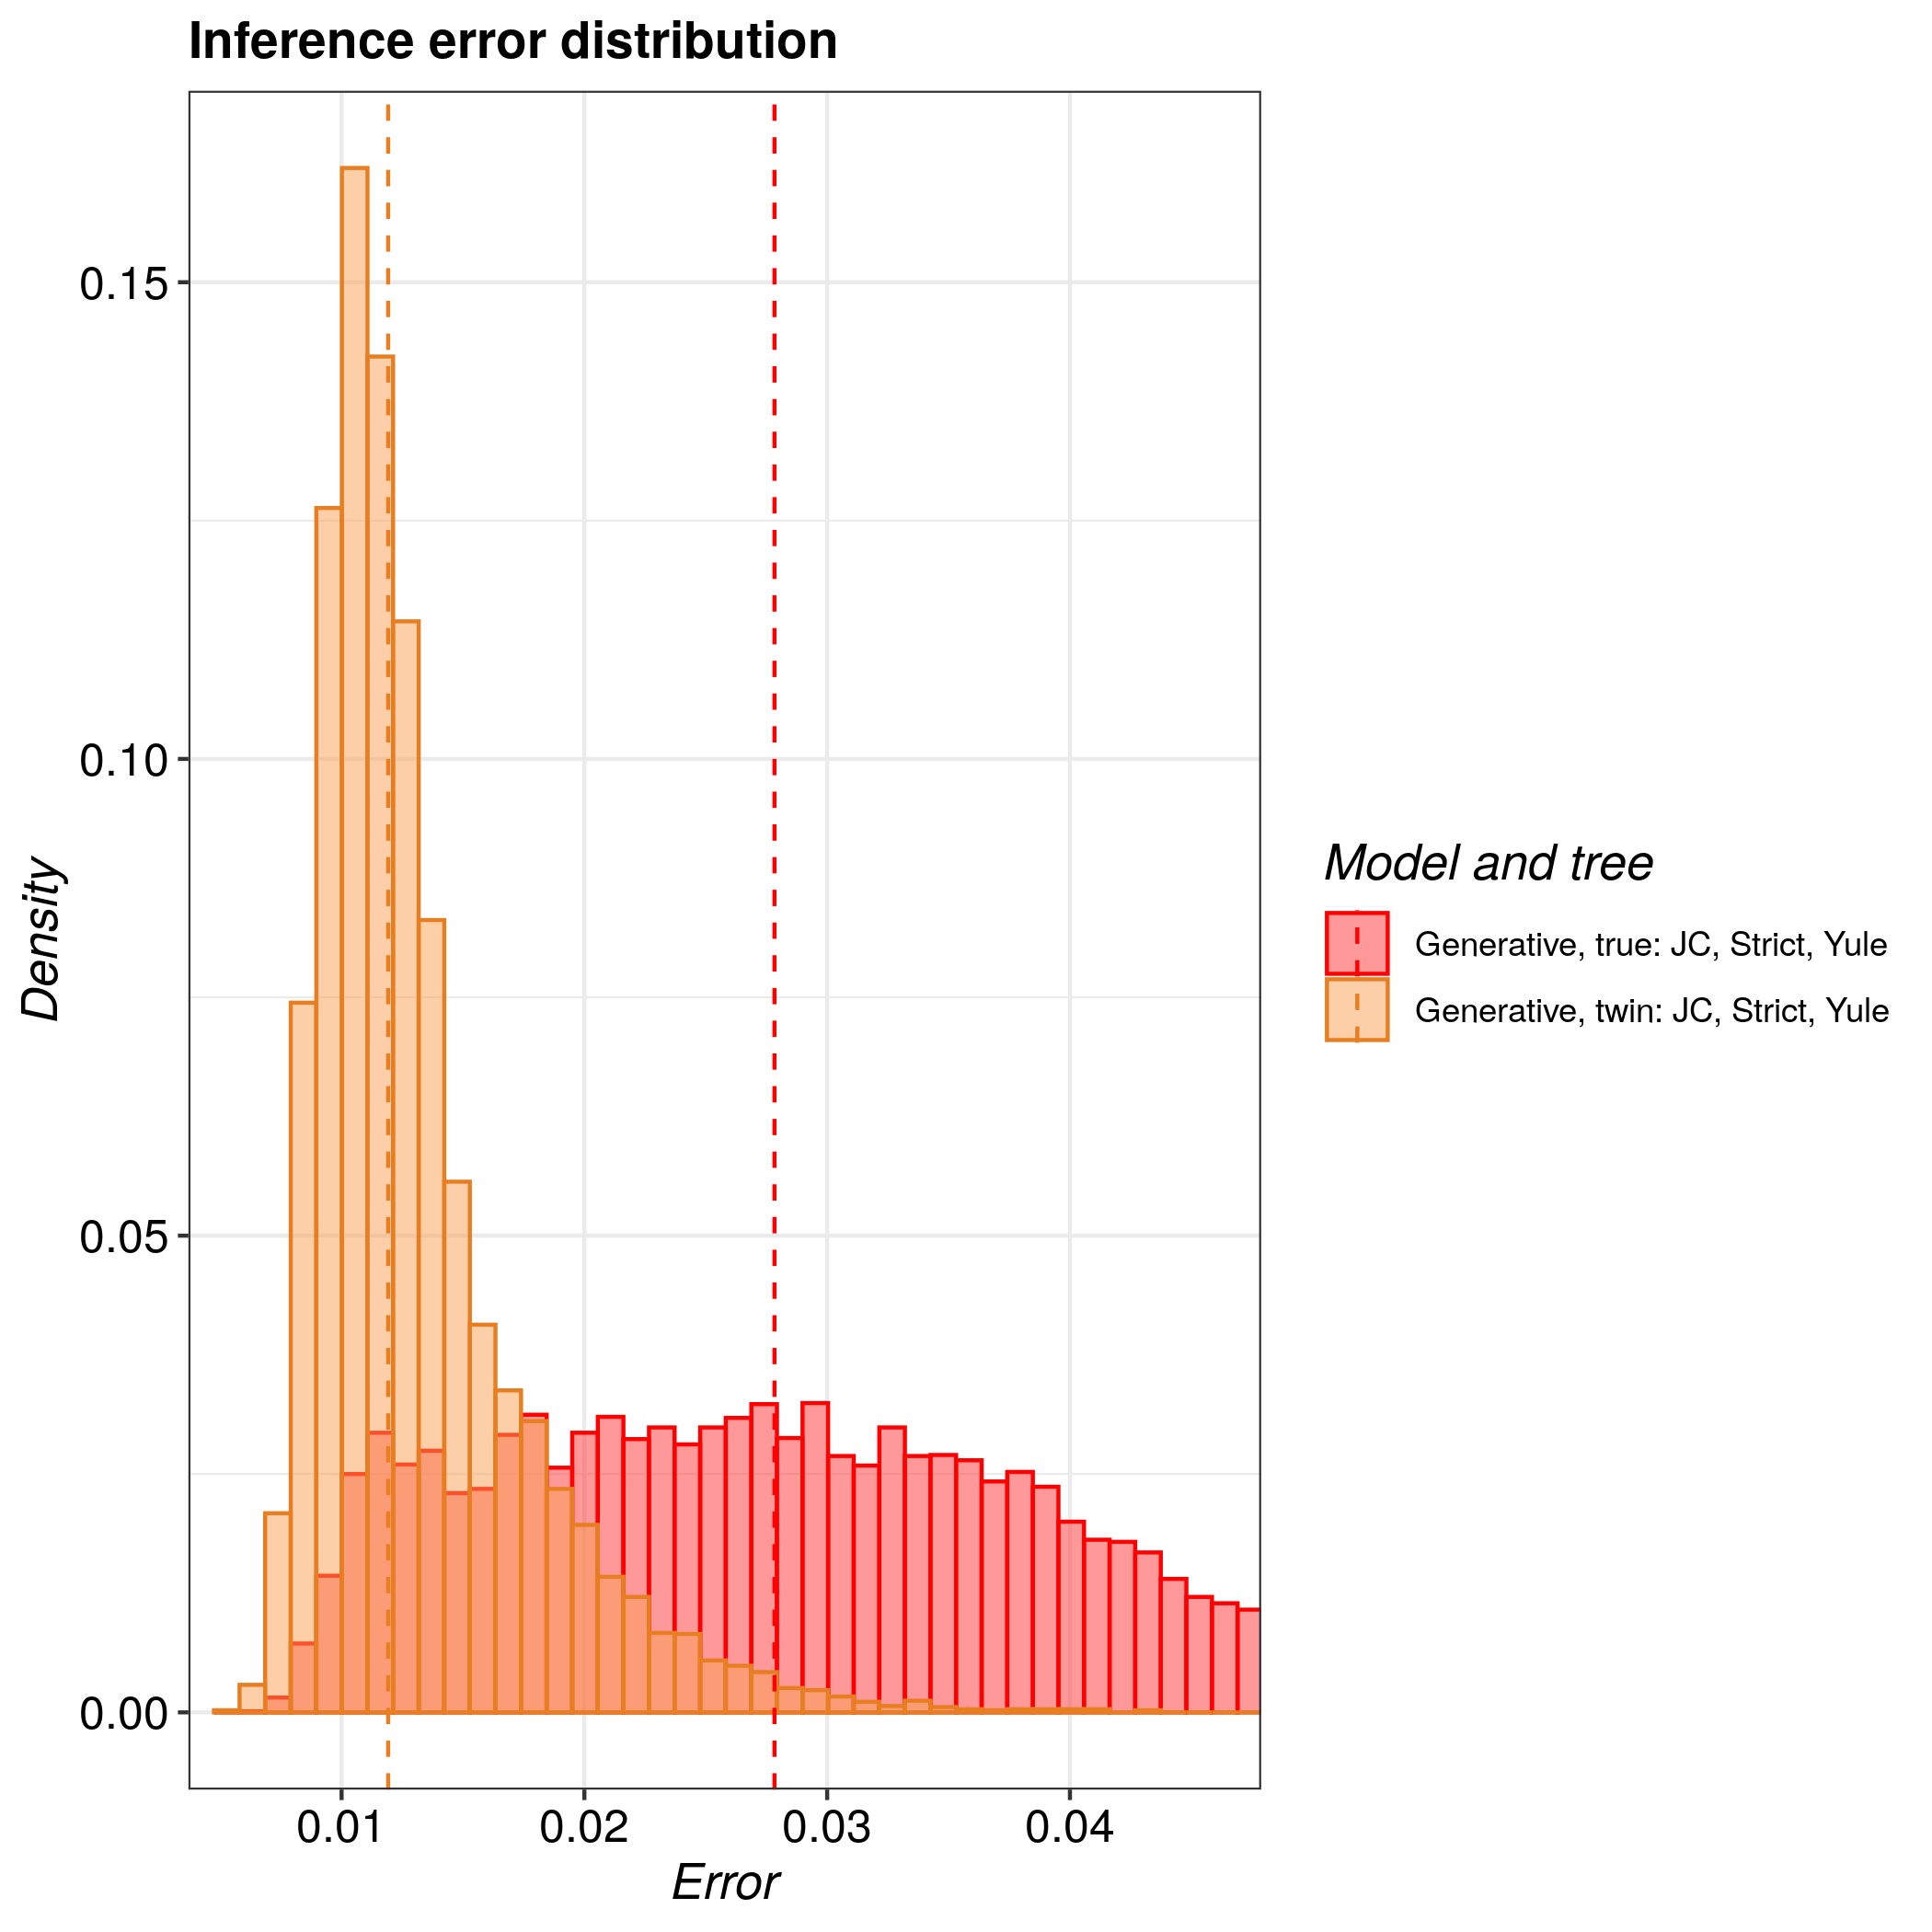
\includegraphics[width=\textwidth]{pirouette_example_20/example_20_317/errors.png}
  \caption{40 taxa}
\end{figure}

%%%%%%%%%%%%%%%%%%%%%%%%%%%%%%%%%%%%%%%%%%%%%%%%%%%%%%%%%%%%%%%%%%%%%%%%%%%%%%%%
\subsection{The effect of DNA sequence length}
%%%%%%%%%%%%%%%%%%%%%%%%%%%%%%%%%%%%%%%%%%%%%%%%%%%%%%%%%%%%%%%%%%%%%%%%%%%%%%%%

The code used in this part of the article can be found at 
\url{https://github.com/richelbilderbeek/pirouette_example_21}.

\begin{figure}[H]
  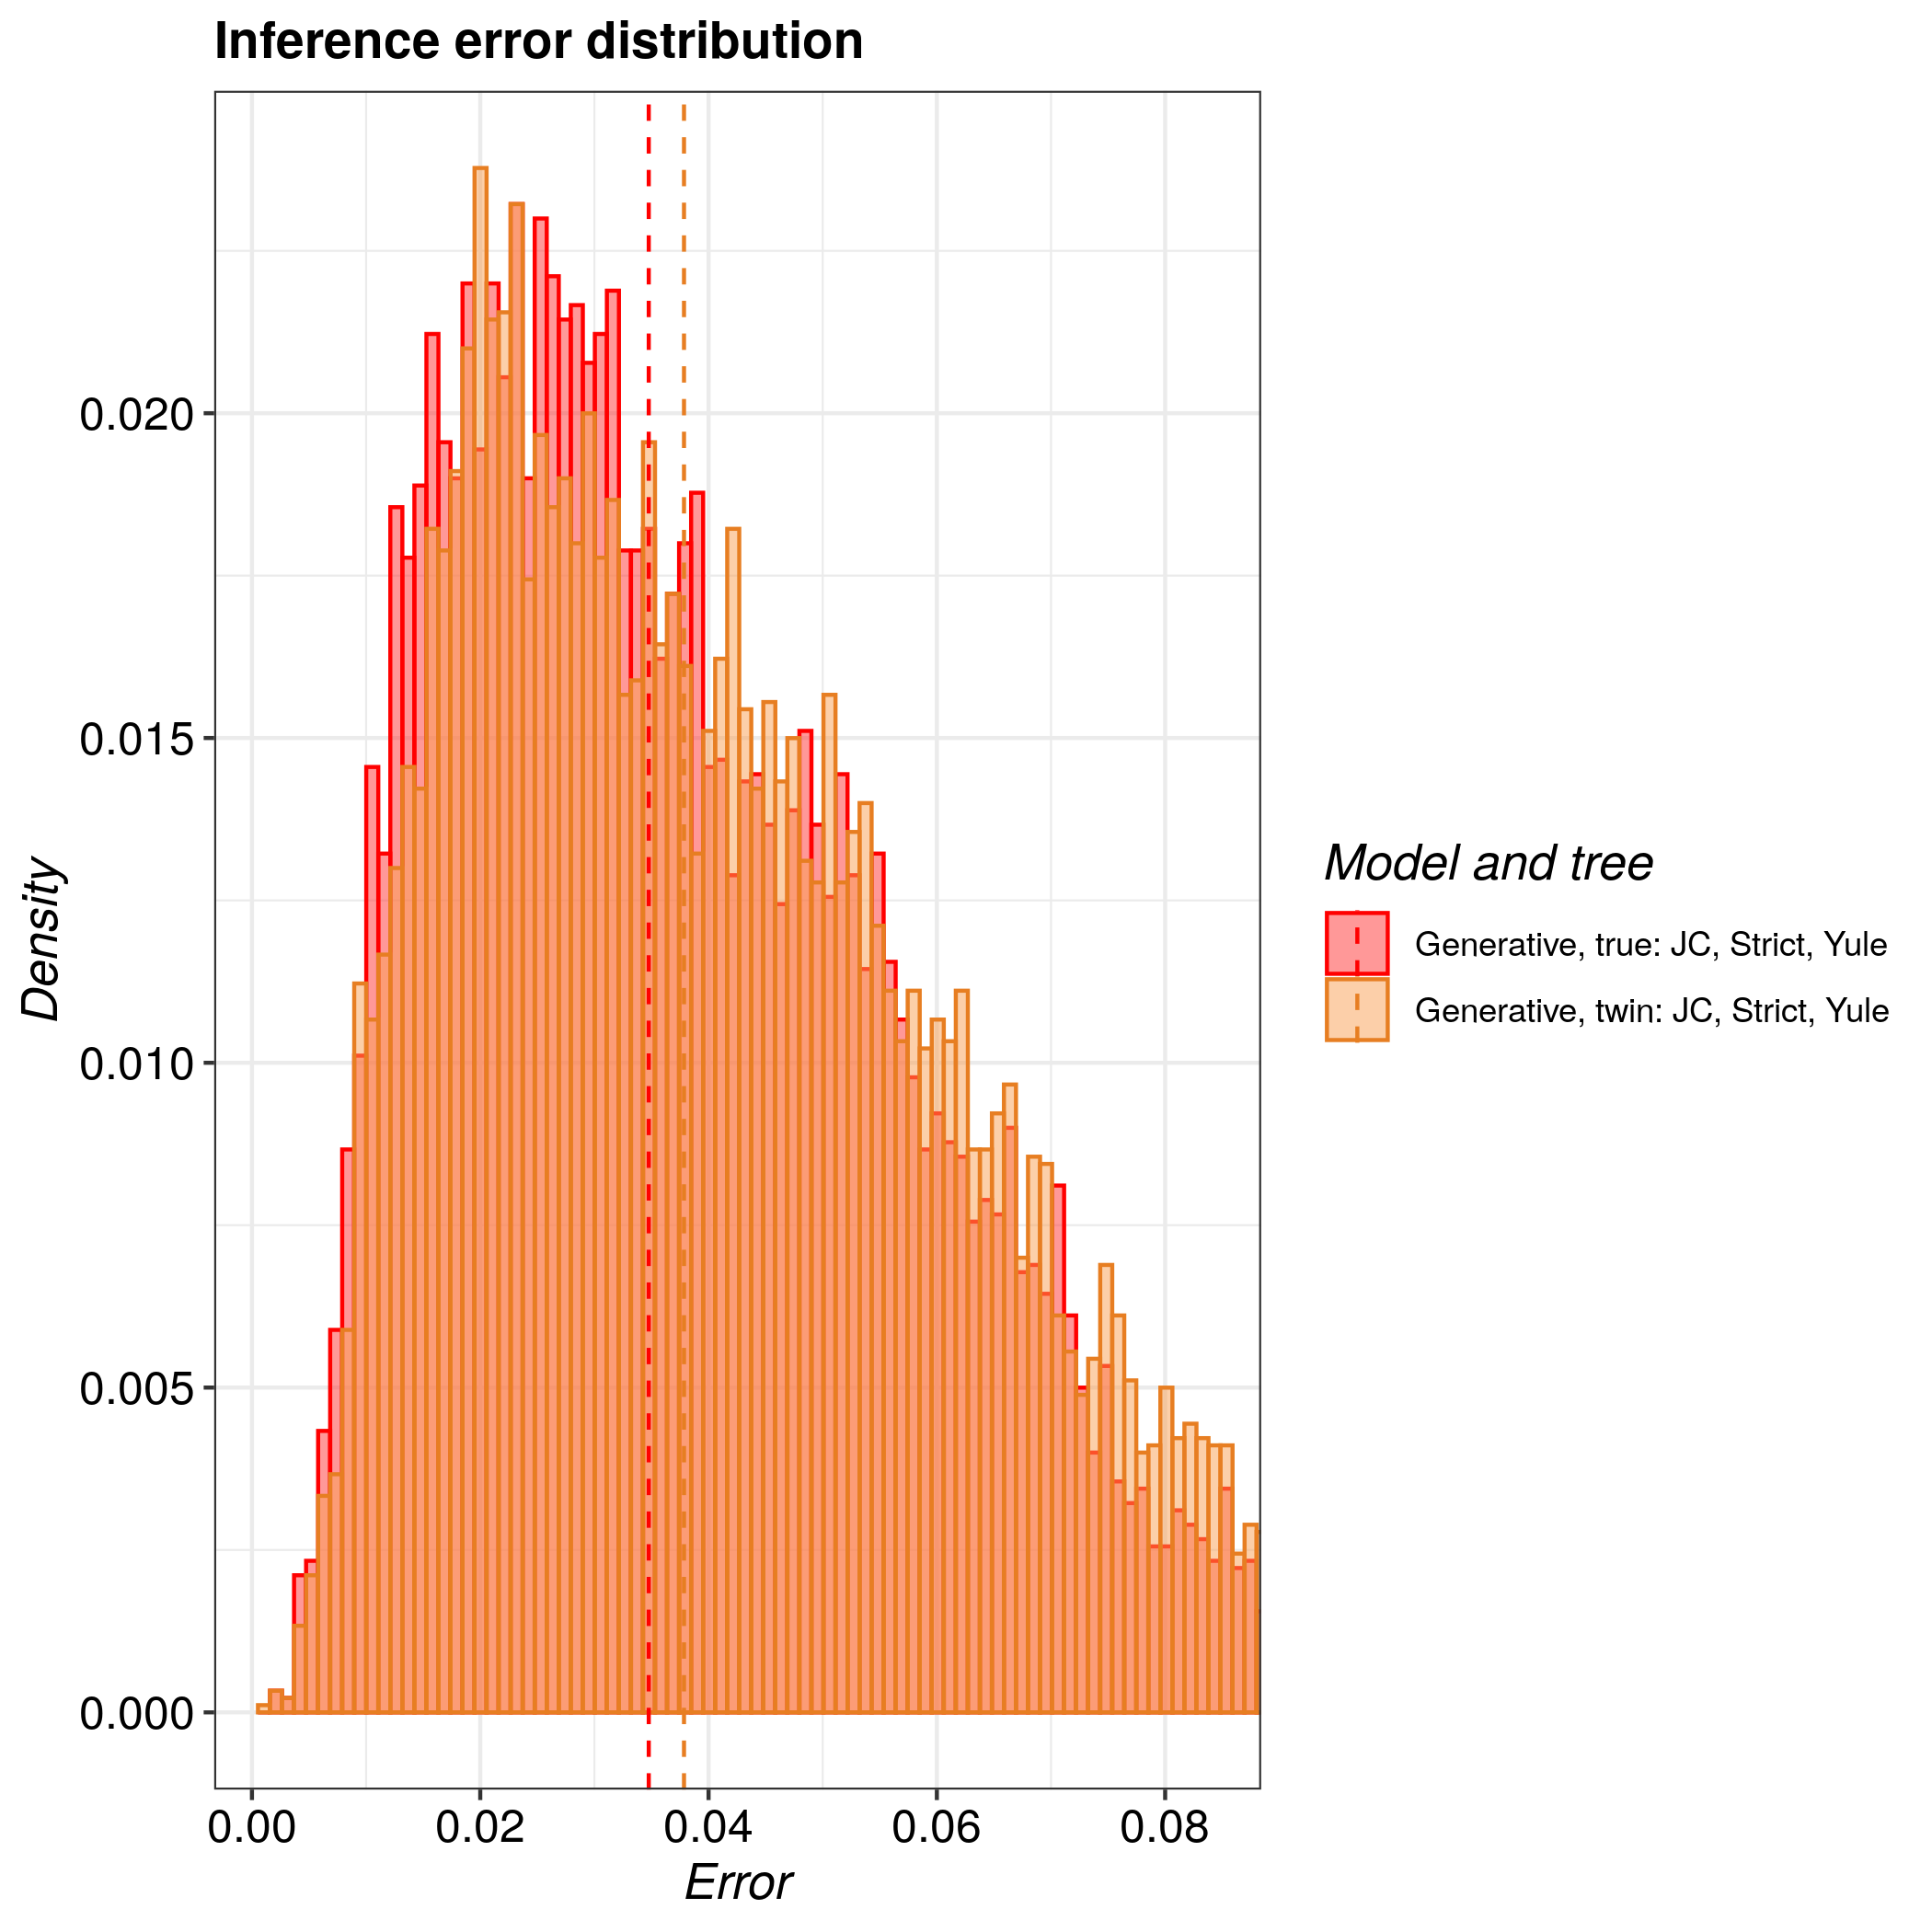
\includegraphics[width=\textwidth]{pirouette_example_21/example_21_314/errors.png}
  \caption{100 nucleotides}
\end{figure}

\begin{figure}[H]
  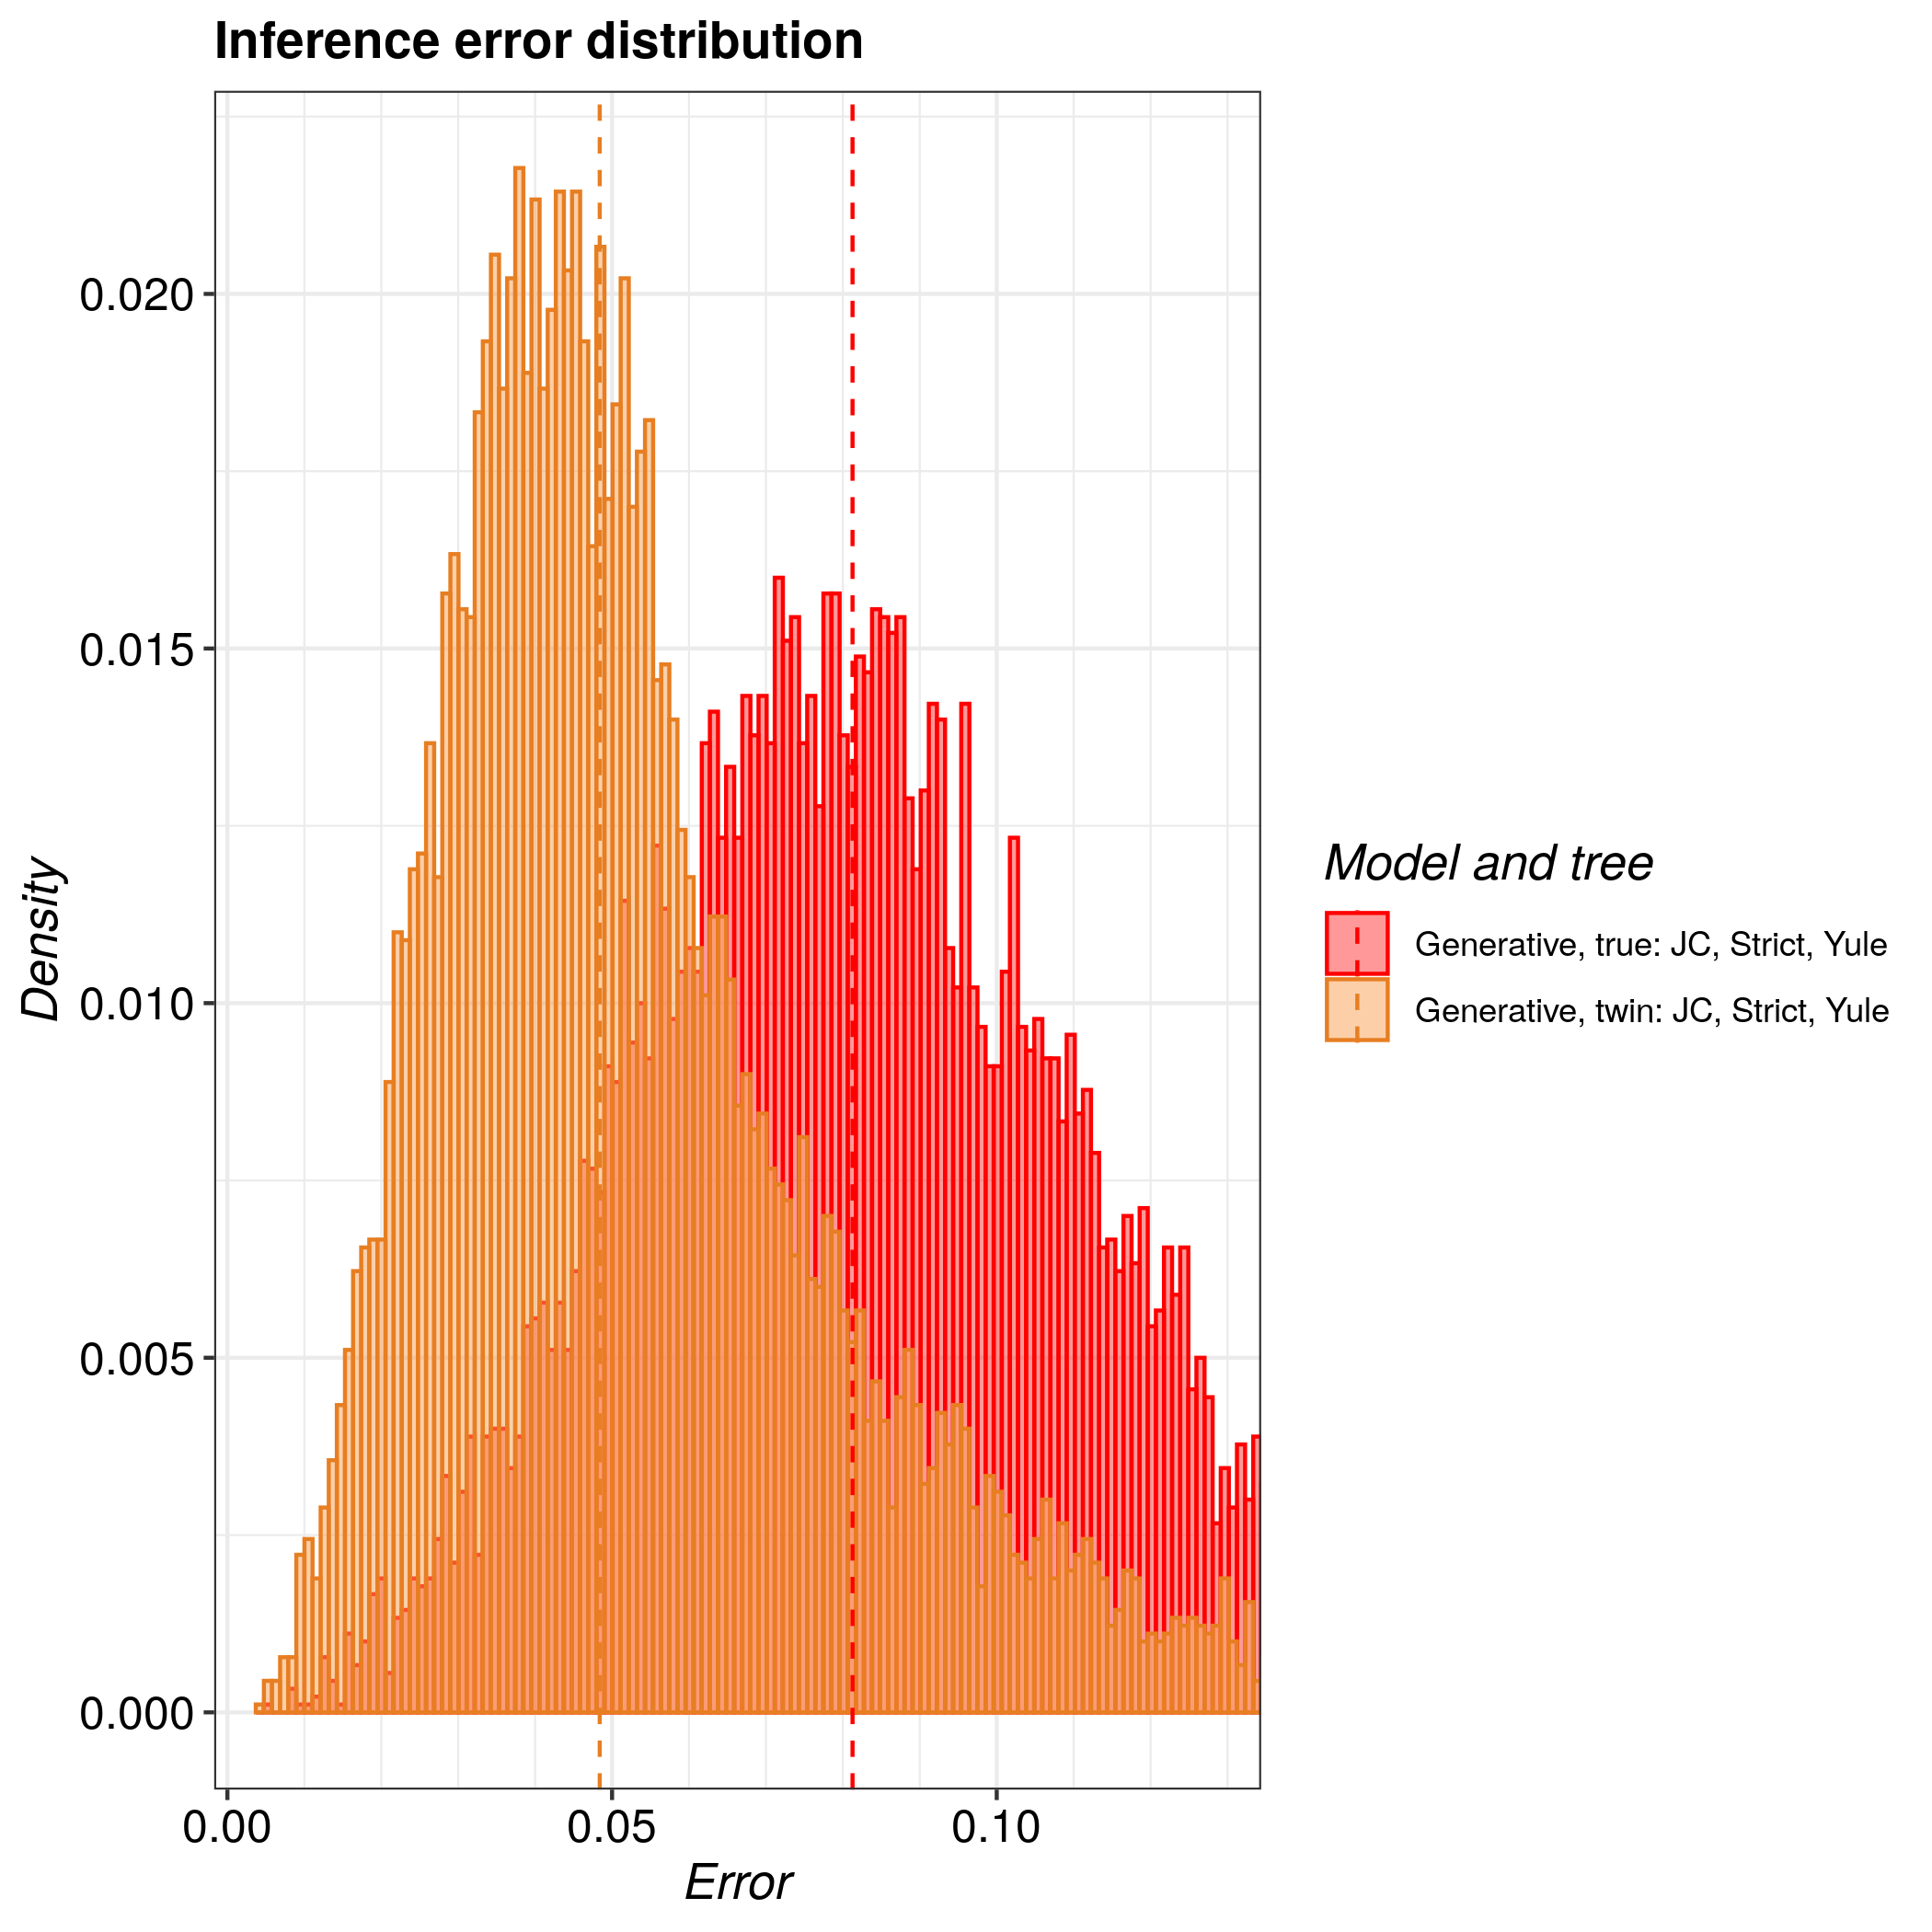
\includegraphics[width=\textwidth]{pirouette_example_21/example_21_315/errors.png}
  \caption{248 nucleotides}
\end{figure}

\begin{figure}[H]
  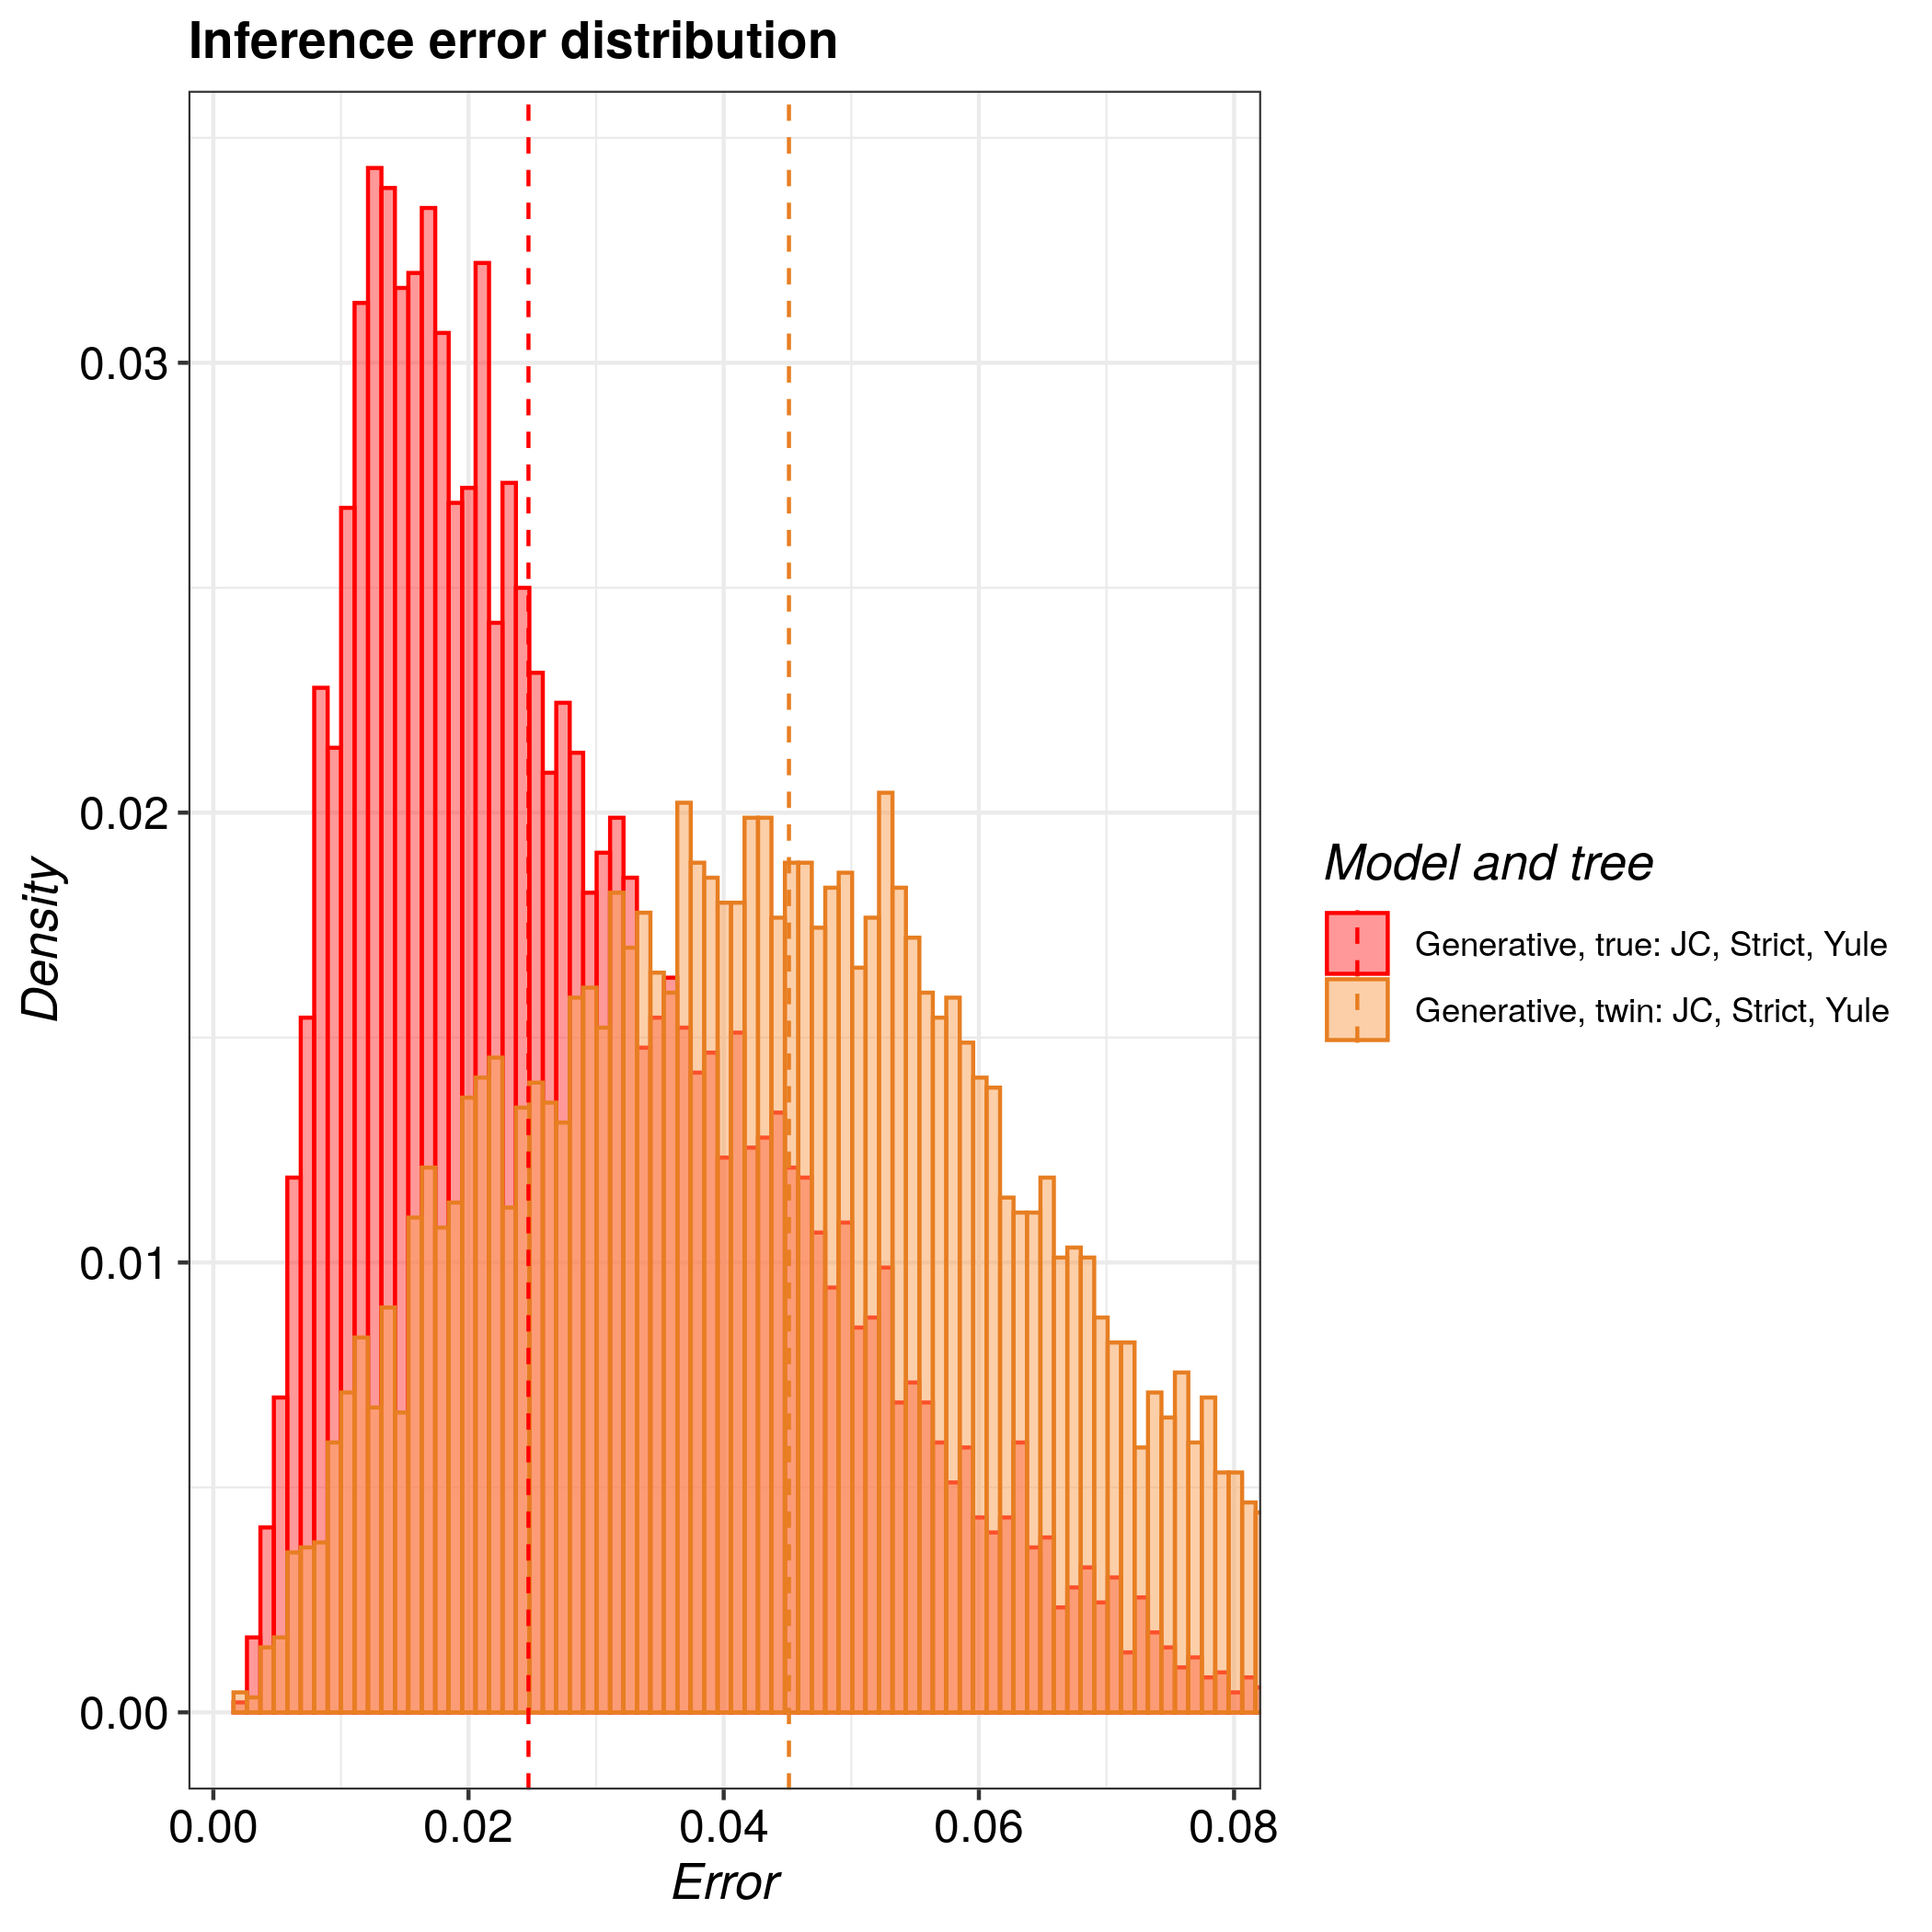
\includegraphics[width=\textwidth]{pirouette_example_21/example_21_316/errors.png}
  \caption{500 nucleotides}
\end{figure}

\begin{figure}[H]
  \includegraphics[width=\textwidth]{pirouette_example_21/example_21_317/errors.png}
  \caption{1000 nucleotides}
\end{figure}

\begin{figure}[H]
  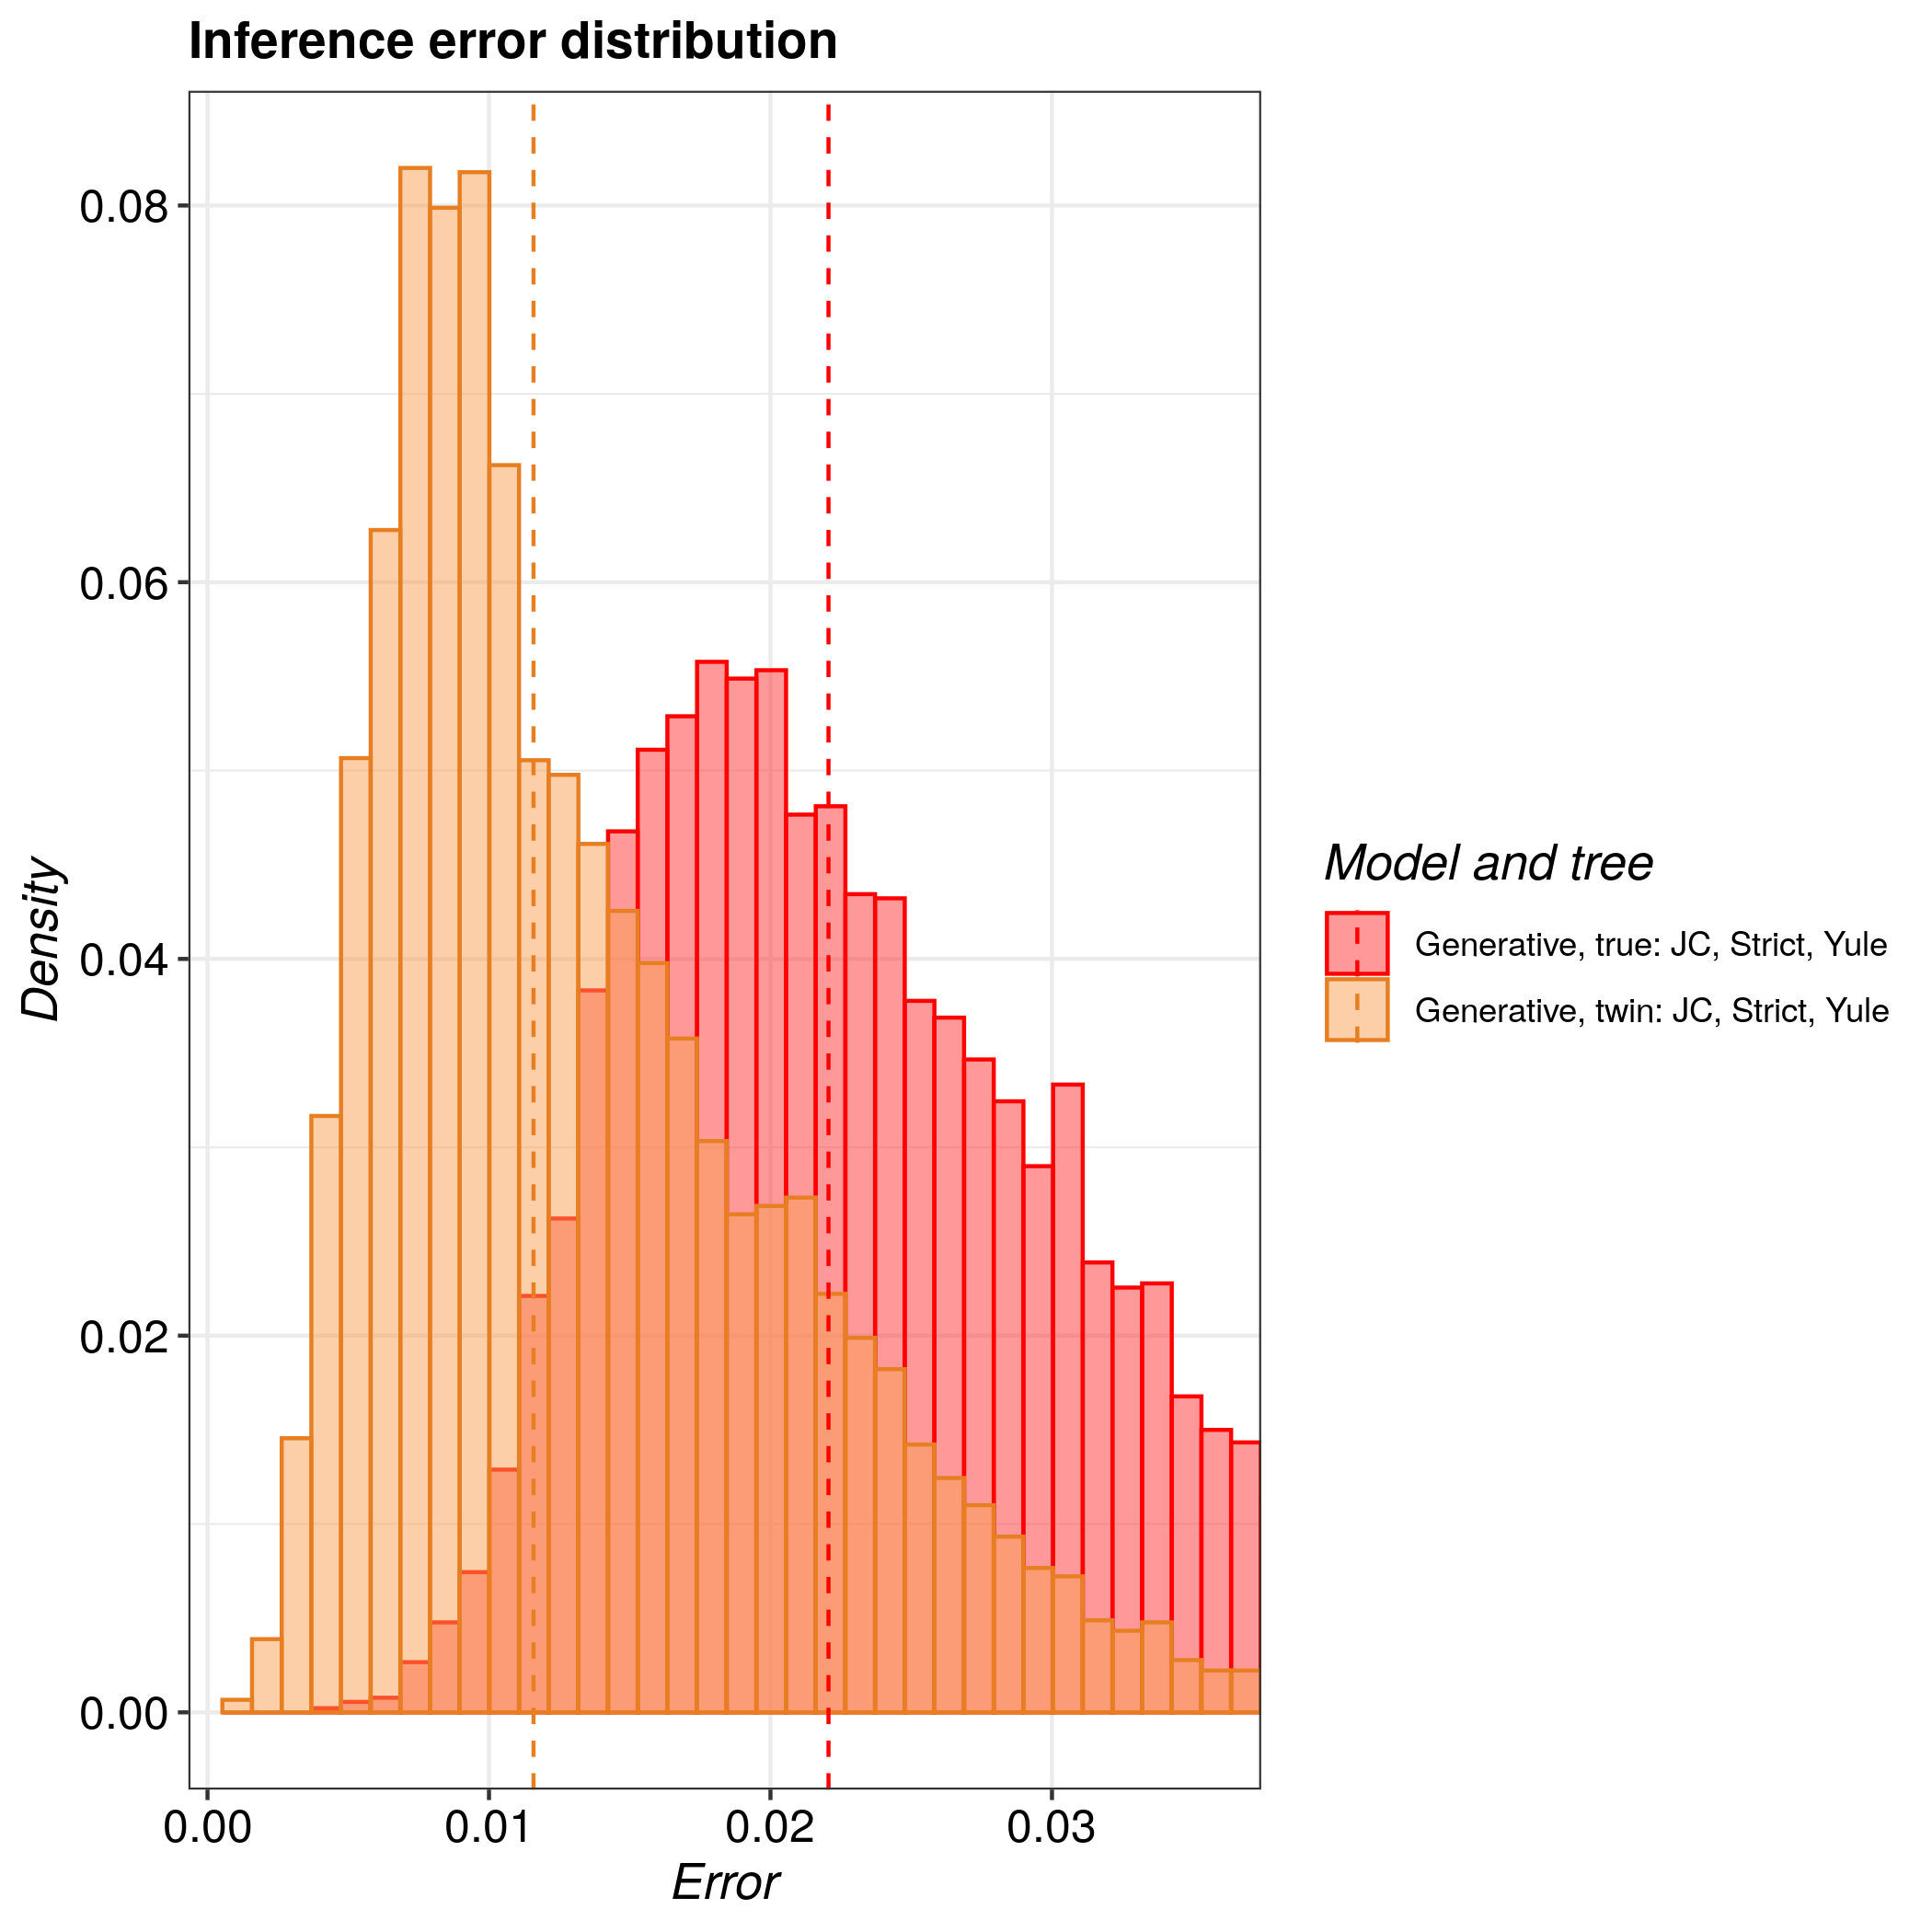
\includegraphics[width=\textwidth]{pirouette_example_21/example_21_318/errors.png}
  \caption{2000 nucleotides}
\end{figure}

\begin{figure}[H]
  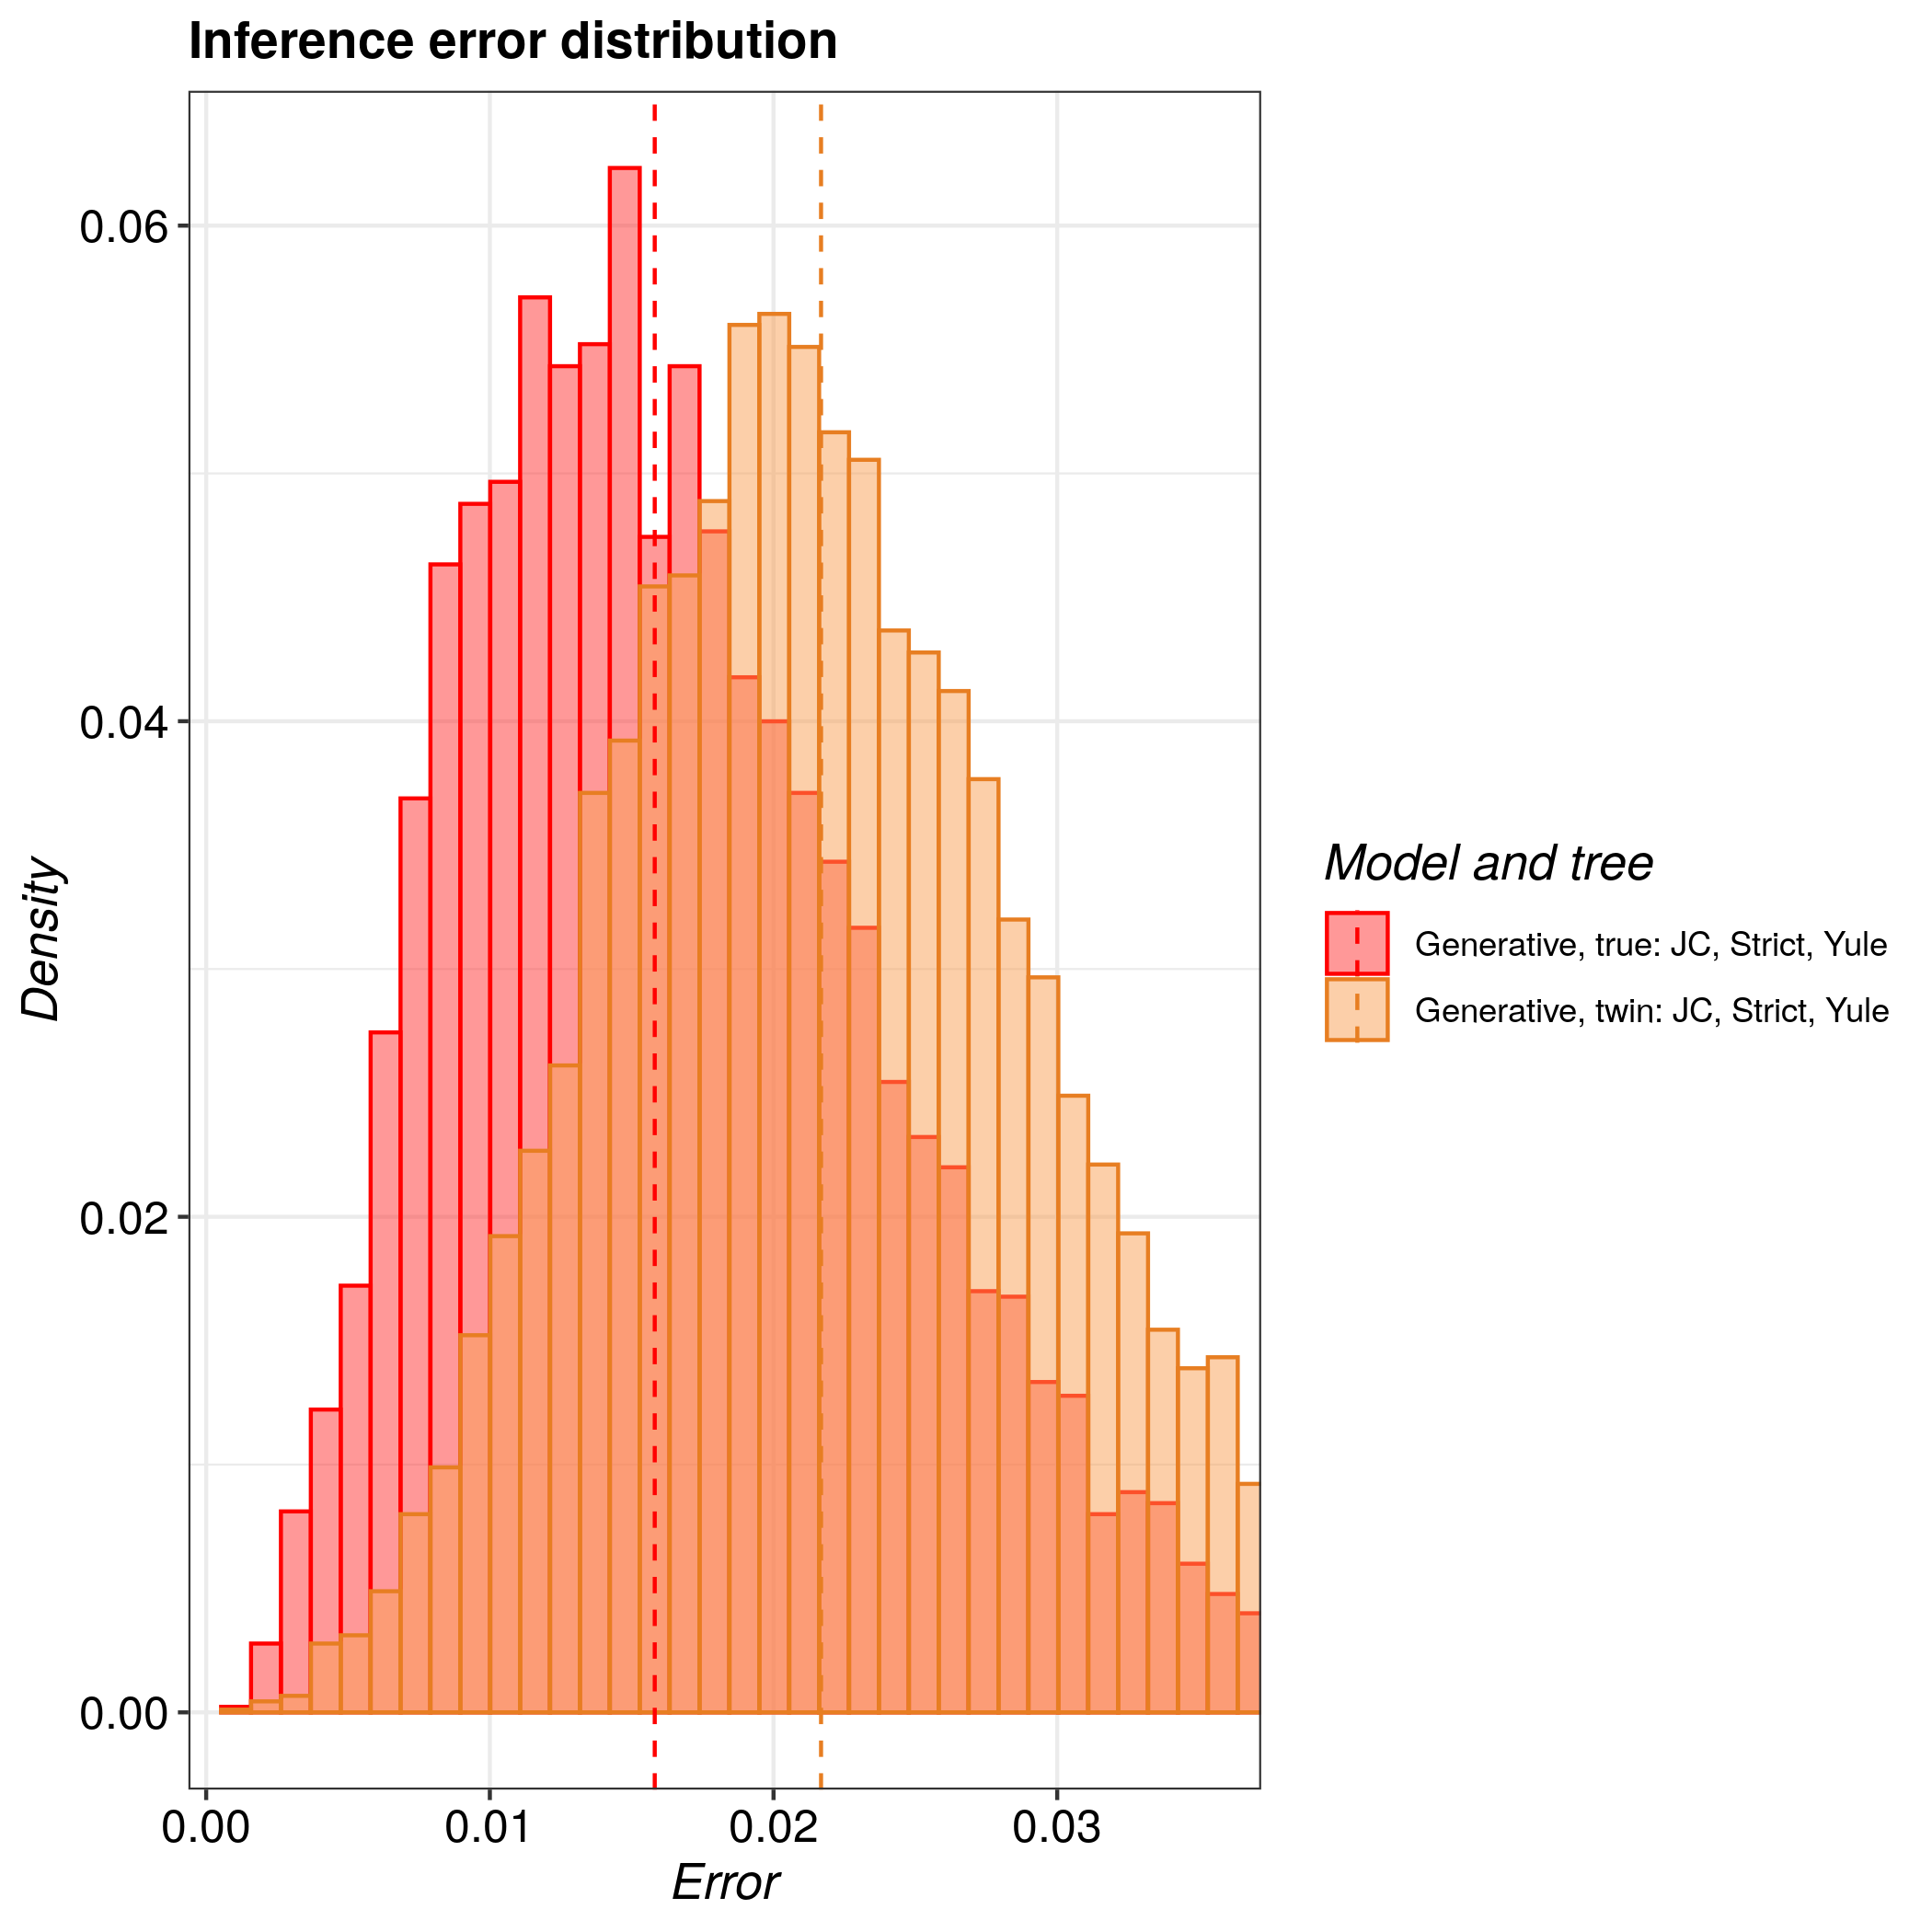
\includegraphics[width=\textwidth]{pirouette_example_21/example_21_319/errors.png}
  \caption{4000 nucleotides}
\end{figure}

\begin{figure}[H]
  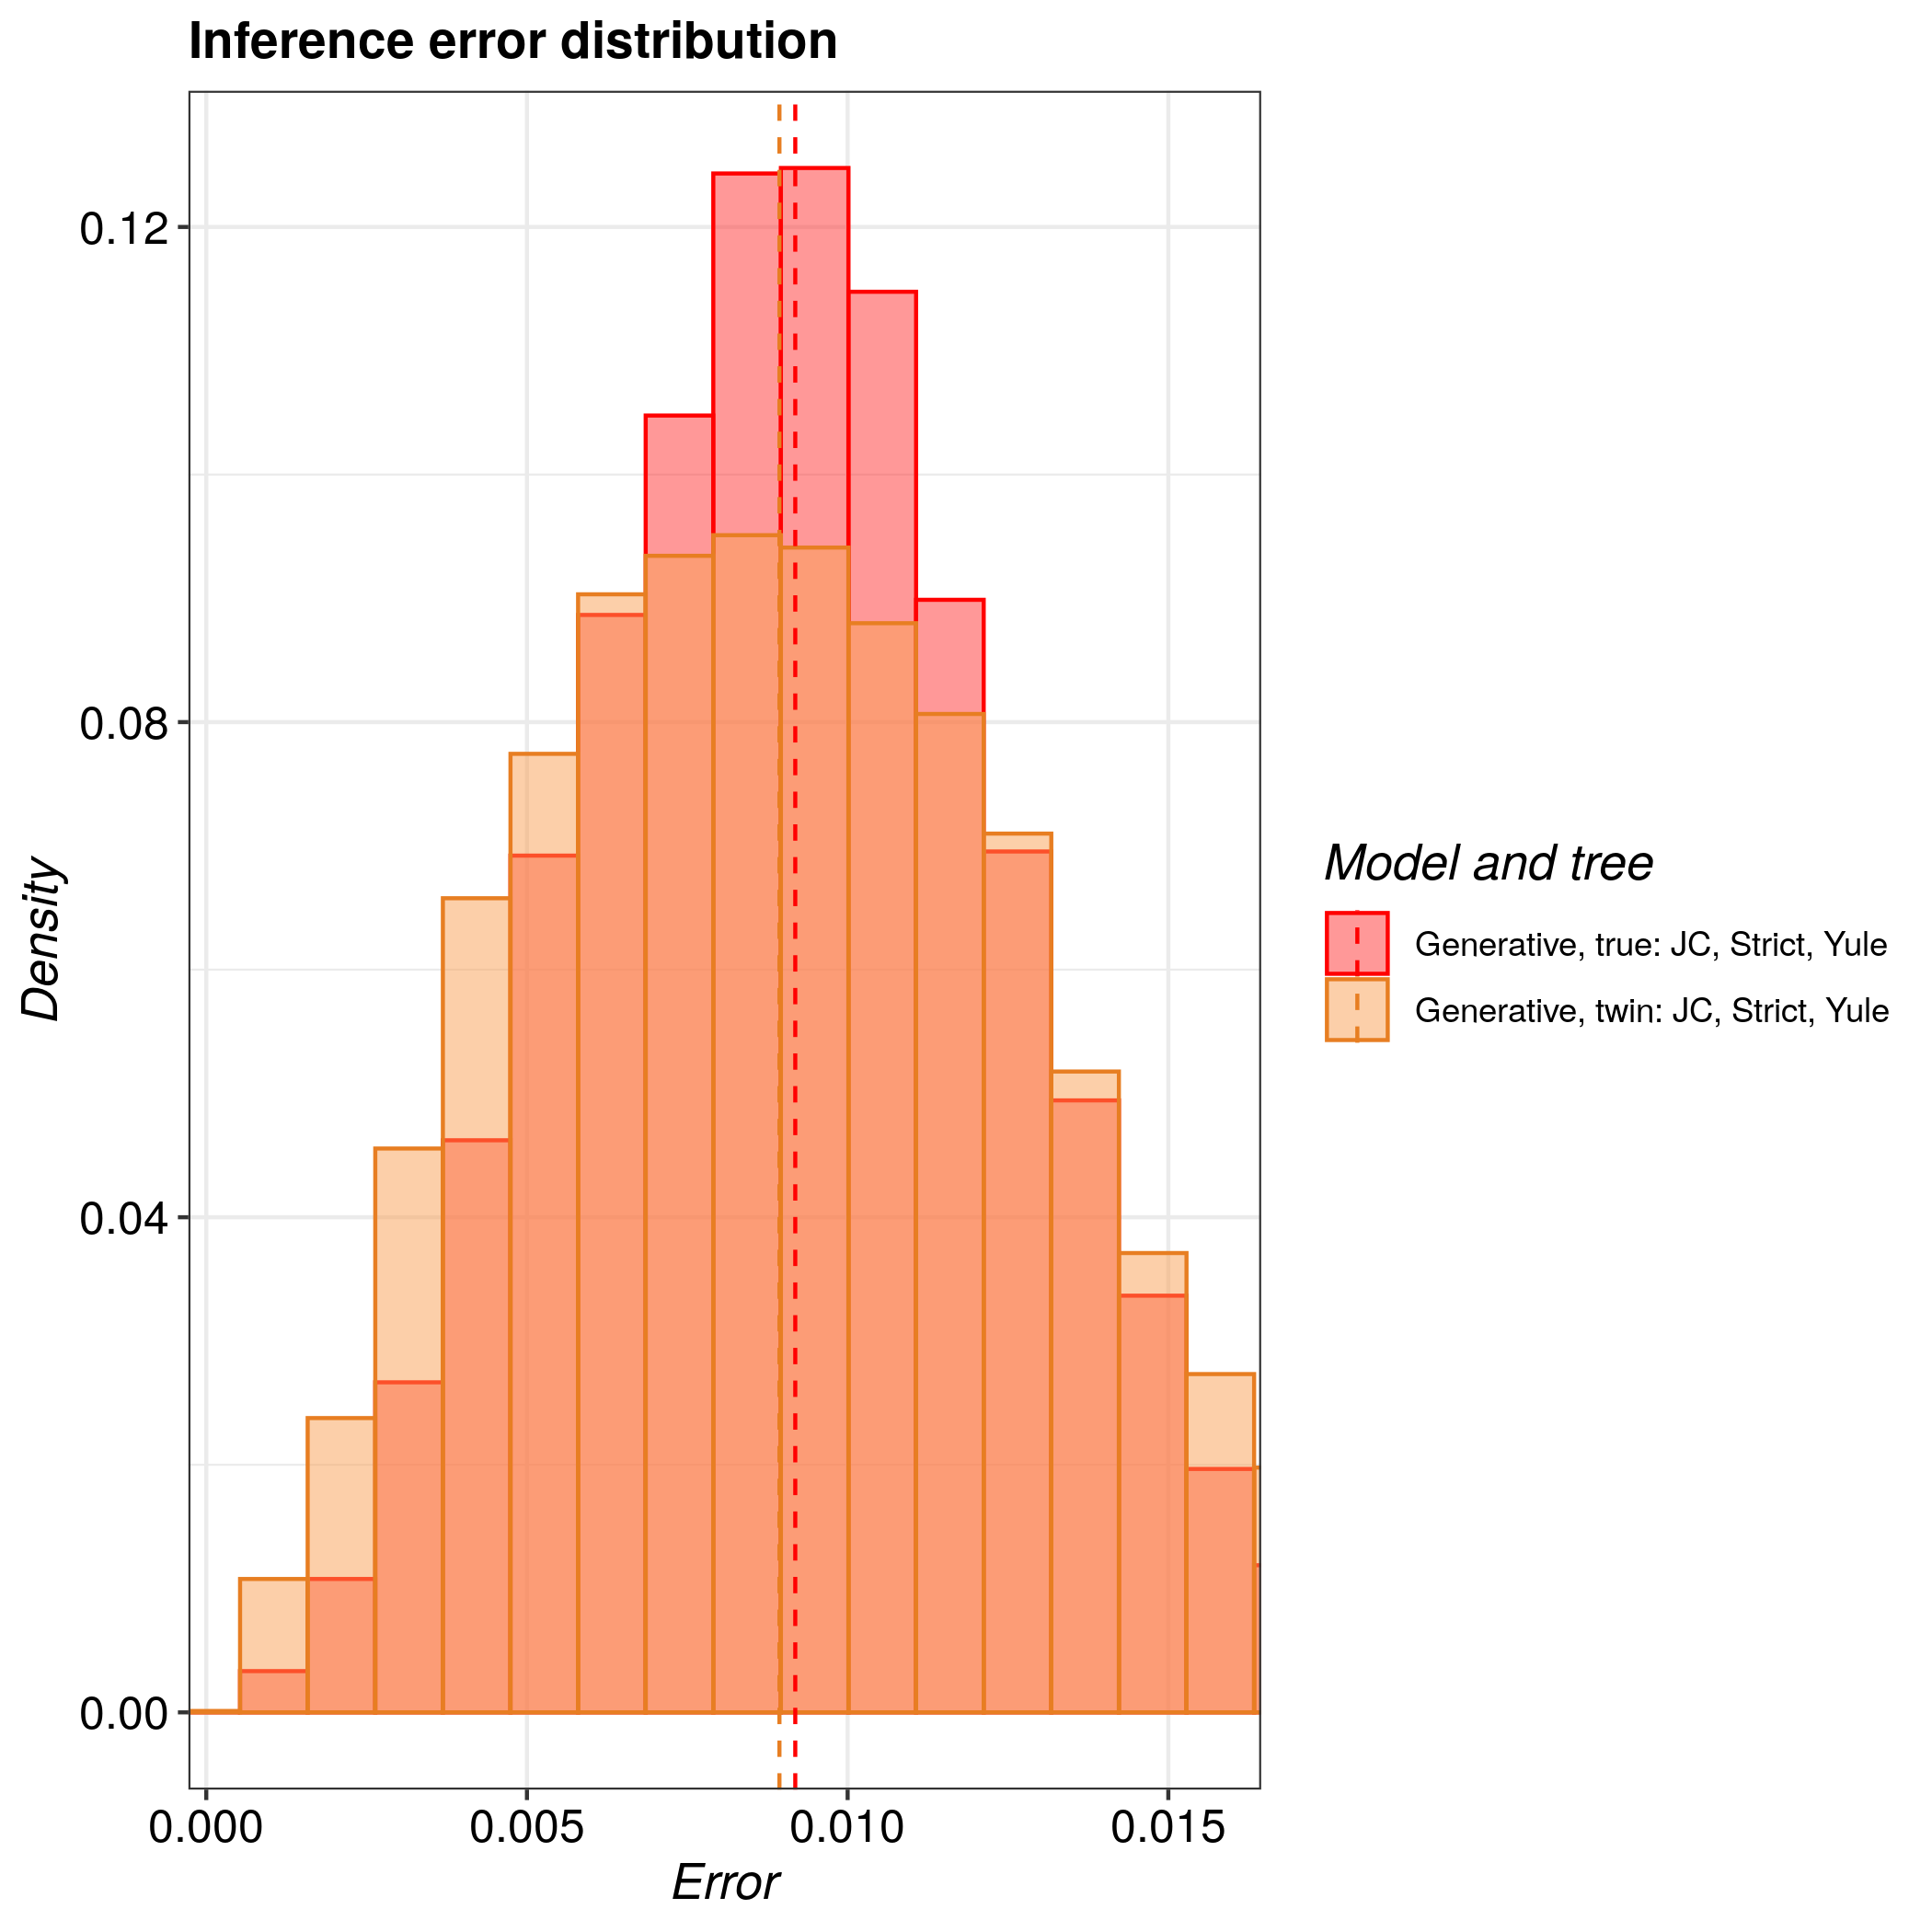
\includegraphics[width=\textwidth]{pirouette_example_21/example_21_320/errors.png}
  \caption{8000 nucleotides}
\end{figure}

\begin{figure}[H]
  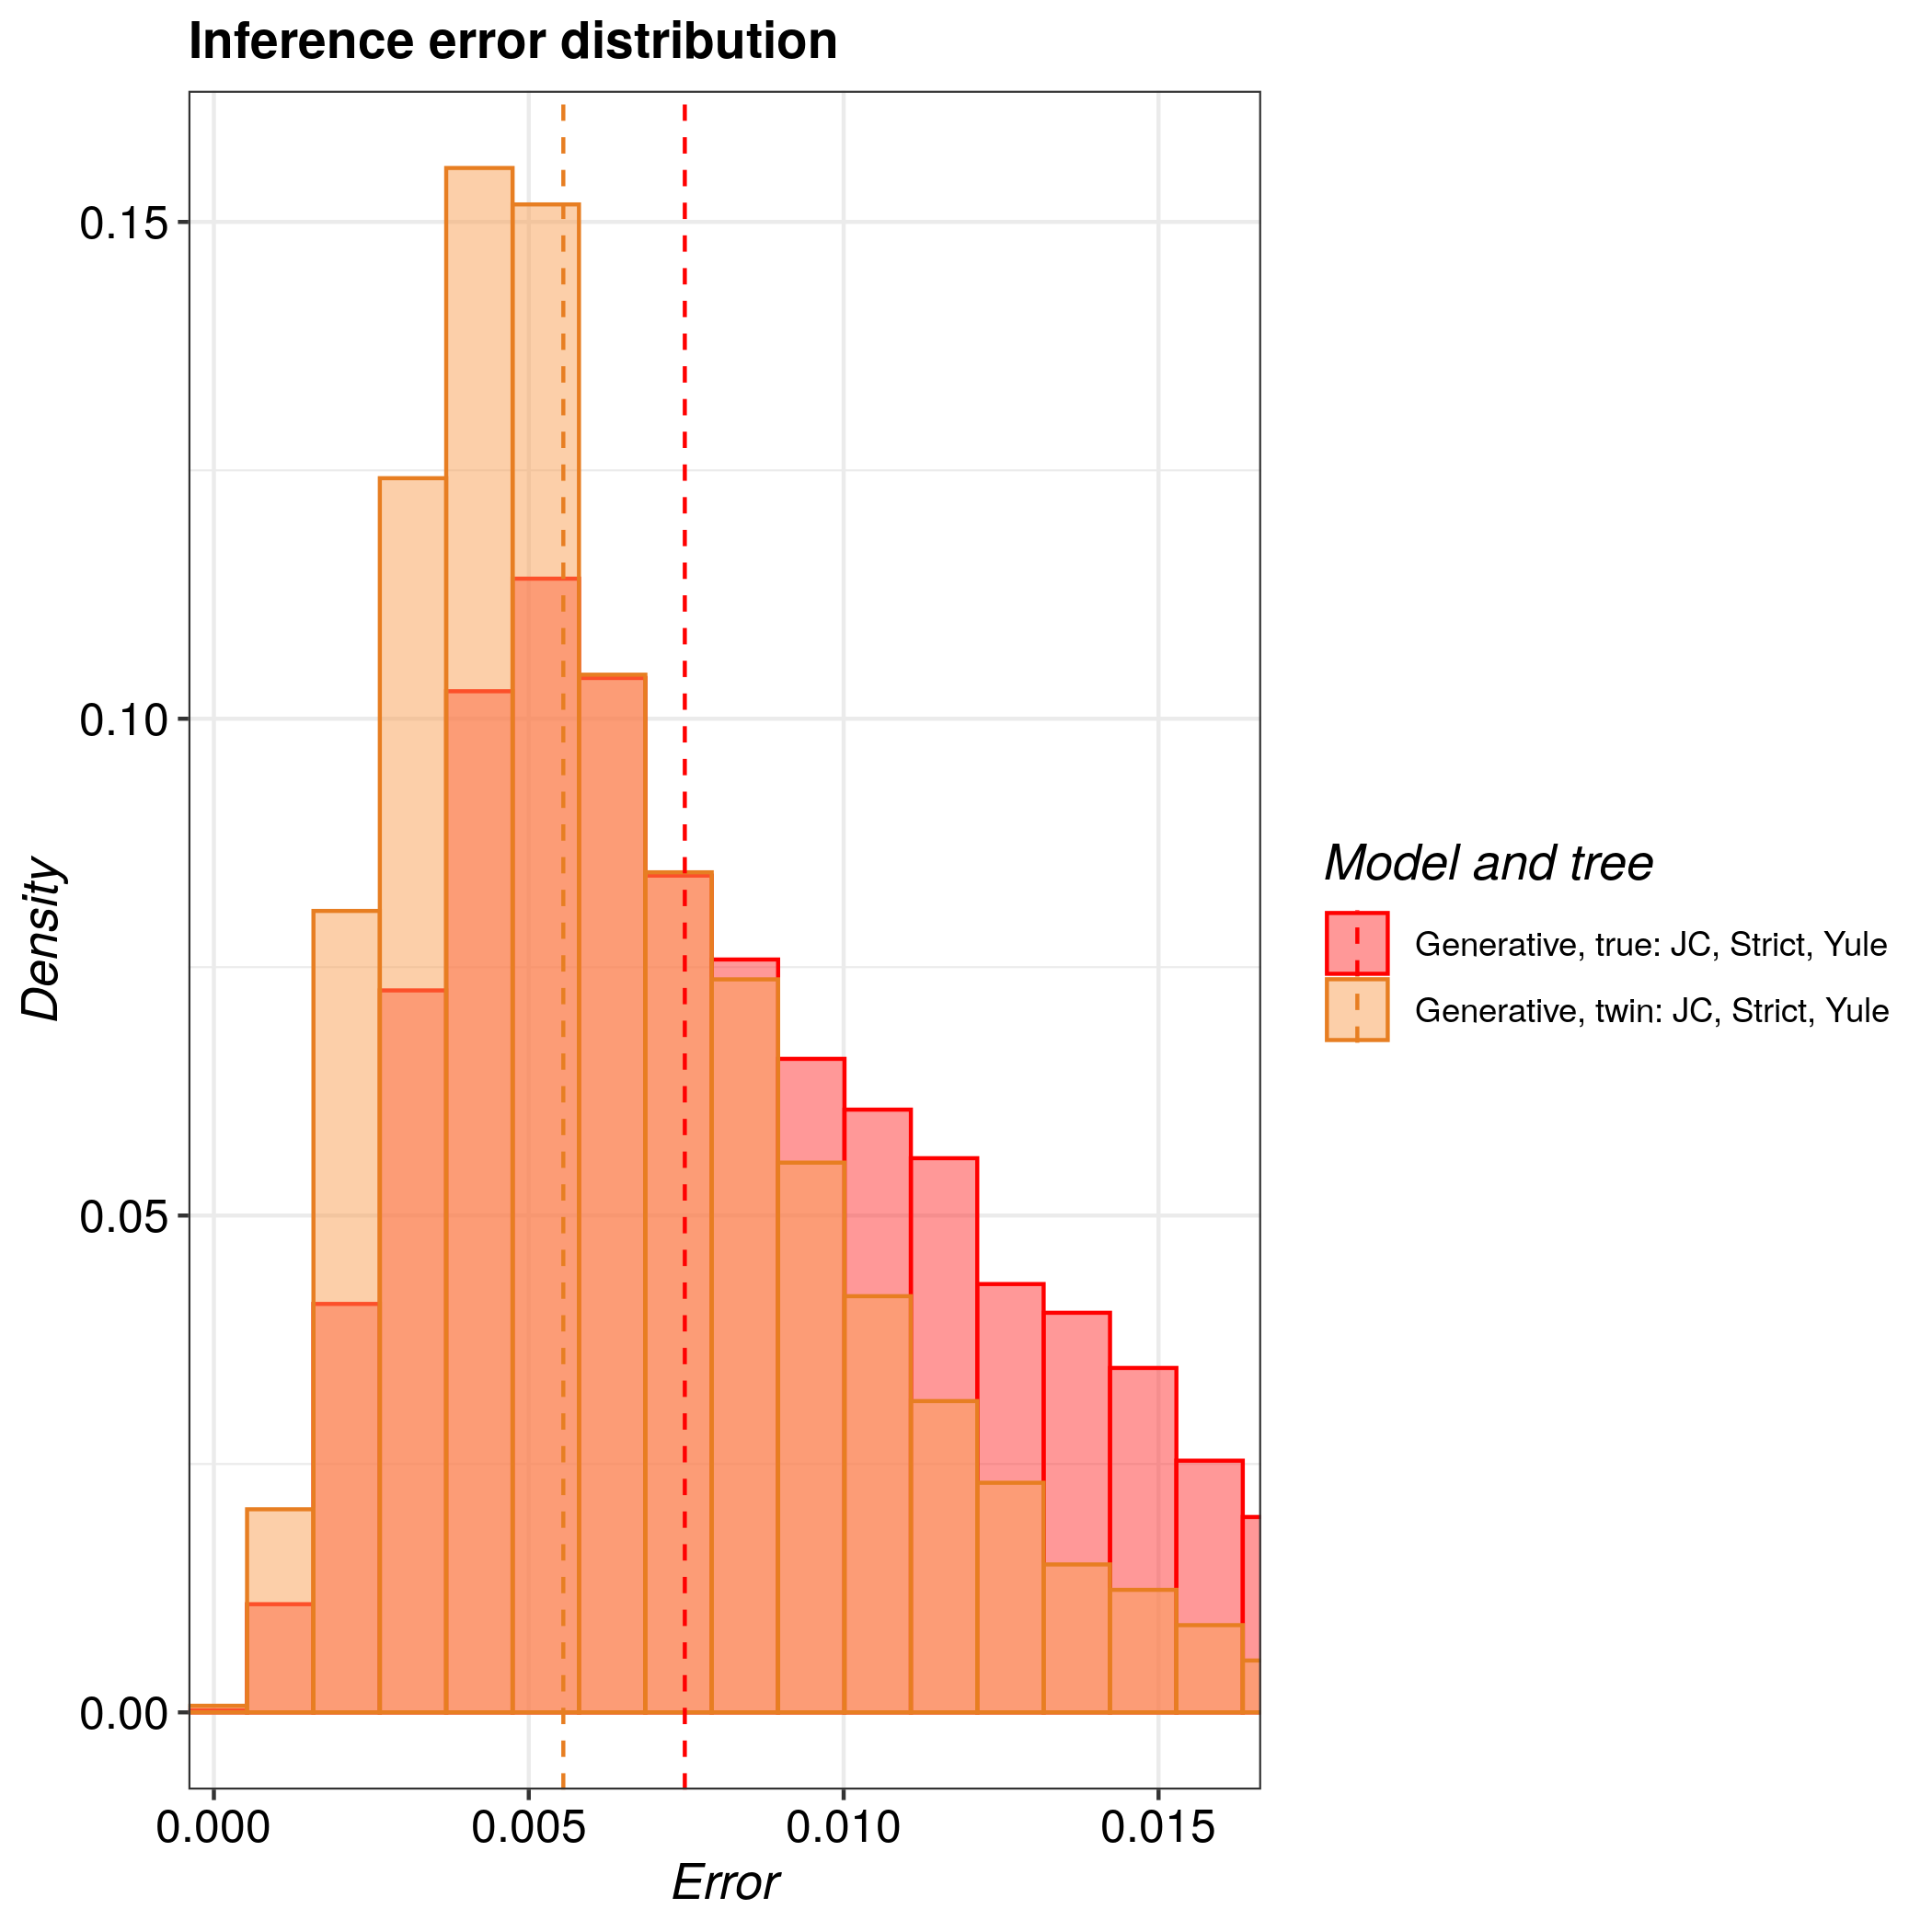
\includegraphics[width=\textwidth]{pirouette_example_21/example_21_321/errors.png}
  \caption{16000 nucleotides}
\end{figure}

%%%%%%%%%%%%%%%%%%%%%%%%%%%%%%%%%%%%%%%%%%%%%%%%%%%%%%%%%%%%%%%%%%%%%%%%%%%%%%%%
\subsection{The effect of non-clock like models}
%%%%%%%%%%%%%%%%%%%%%%%%%%%%%%%%%%%%%%%%%%%%%%%%%%%%%%%%%%%%%%%%%%%%%%%%%%%%%%%%

The code used in this part of the article can be found at 
\url{https://github.com/richelbilderbeek/pirouette_example_3007}.

\begin{figure}[H]
  \includegraphics[width=\textwidth]{pirouette_example_3007/example_17_314/errors.png}
  \caption{An unliked node substitution model}
\end{figure}

%%%%%%%%%%%%%%%%%%%%%%%%%%%%%%%%%%%%%%%%%%%%%%%%%%%%%%%%%%%%%%%%%%%%%%%%%%%%%%%%
\subsection{The effect of assuming a Yule tree prior on a Yule tree}
%%%%%%%%%%%%%%%%%%%%%%%%%%%%%%%%%%%%%%%%%%%%%%%%%%%%%%%%%%%%%%%%%%%%%%%%%%%%%%%%

The code used in this part of the article can be found at 
\url{https://github.com/richelbilderbeek/pirouette_example_22}.

\begin{figure}[H]
  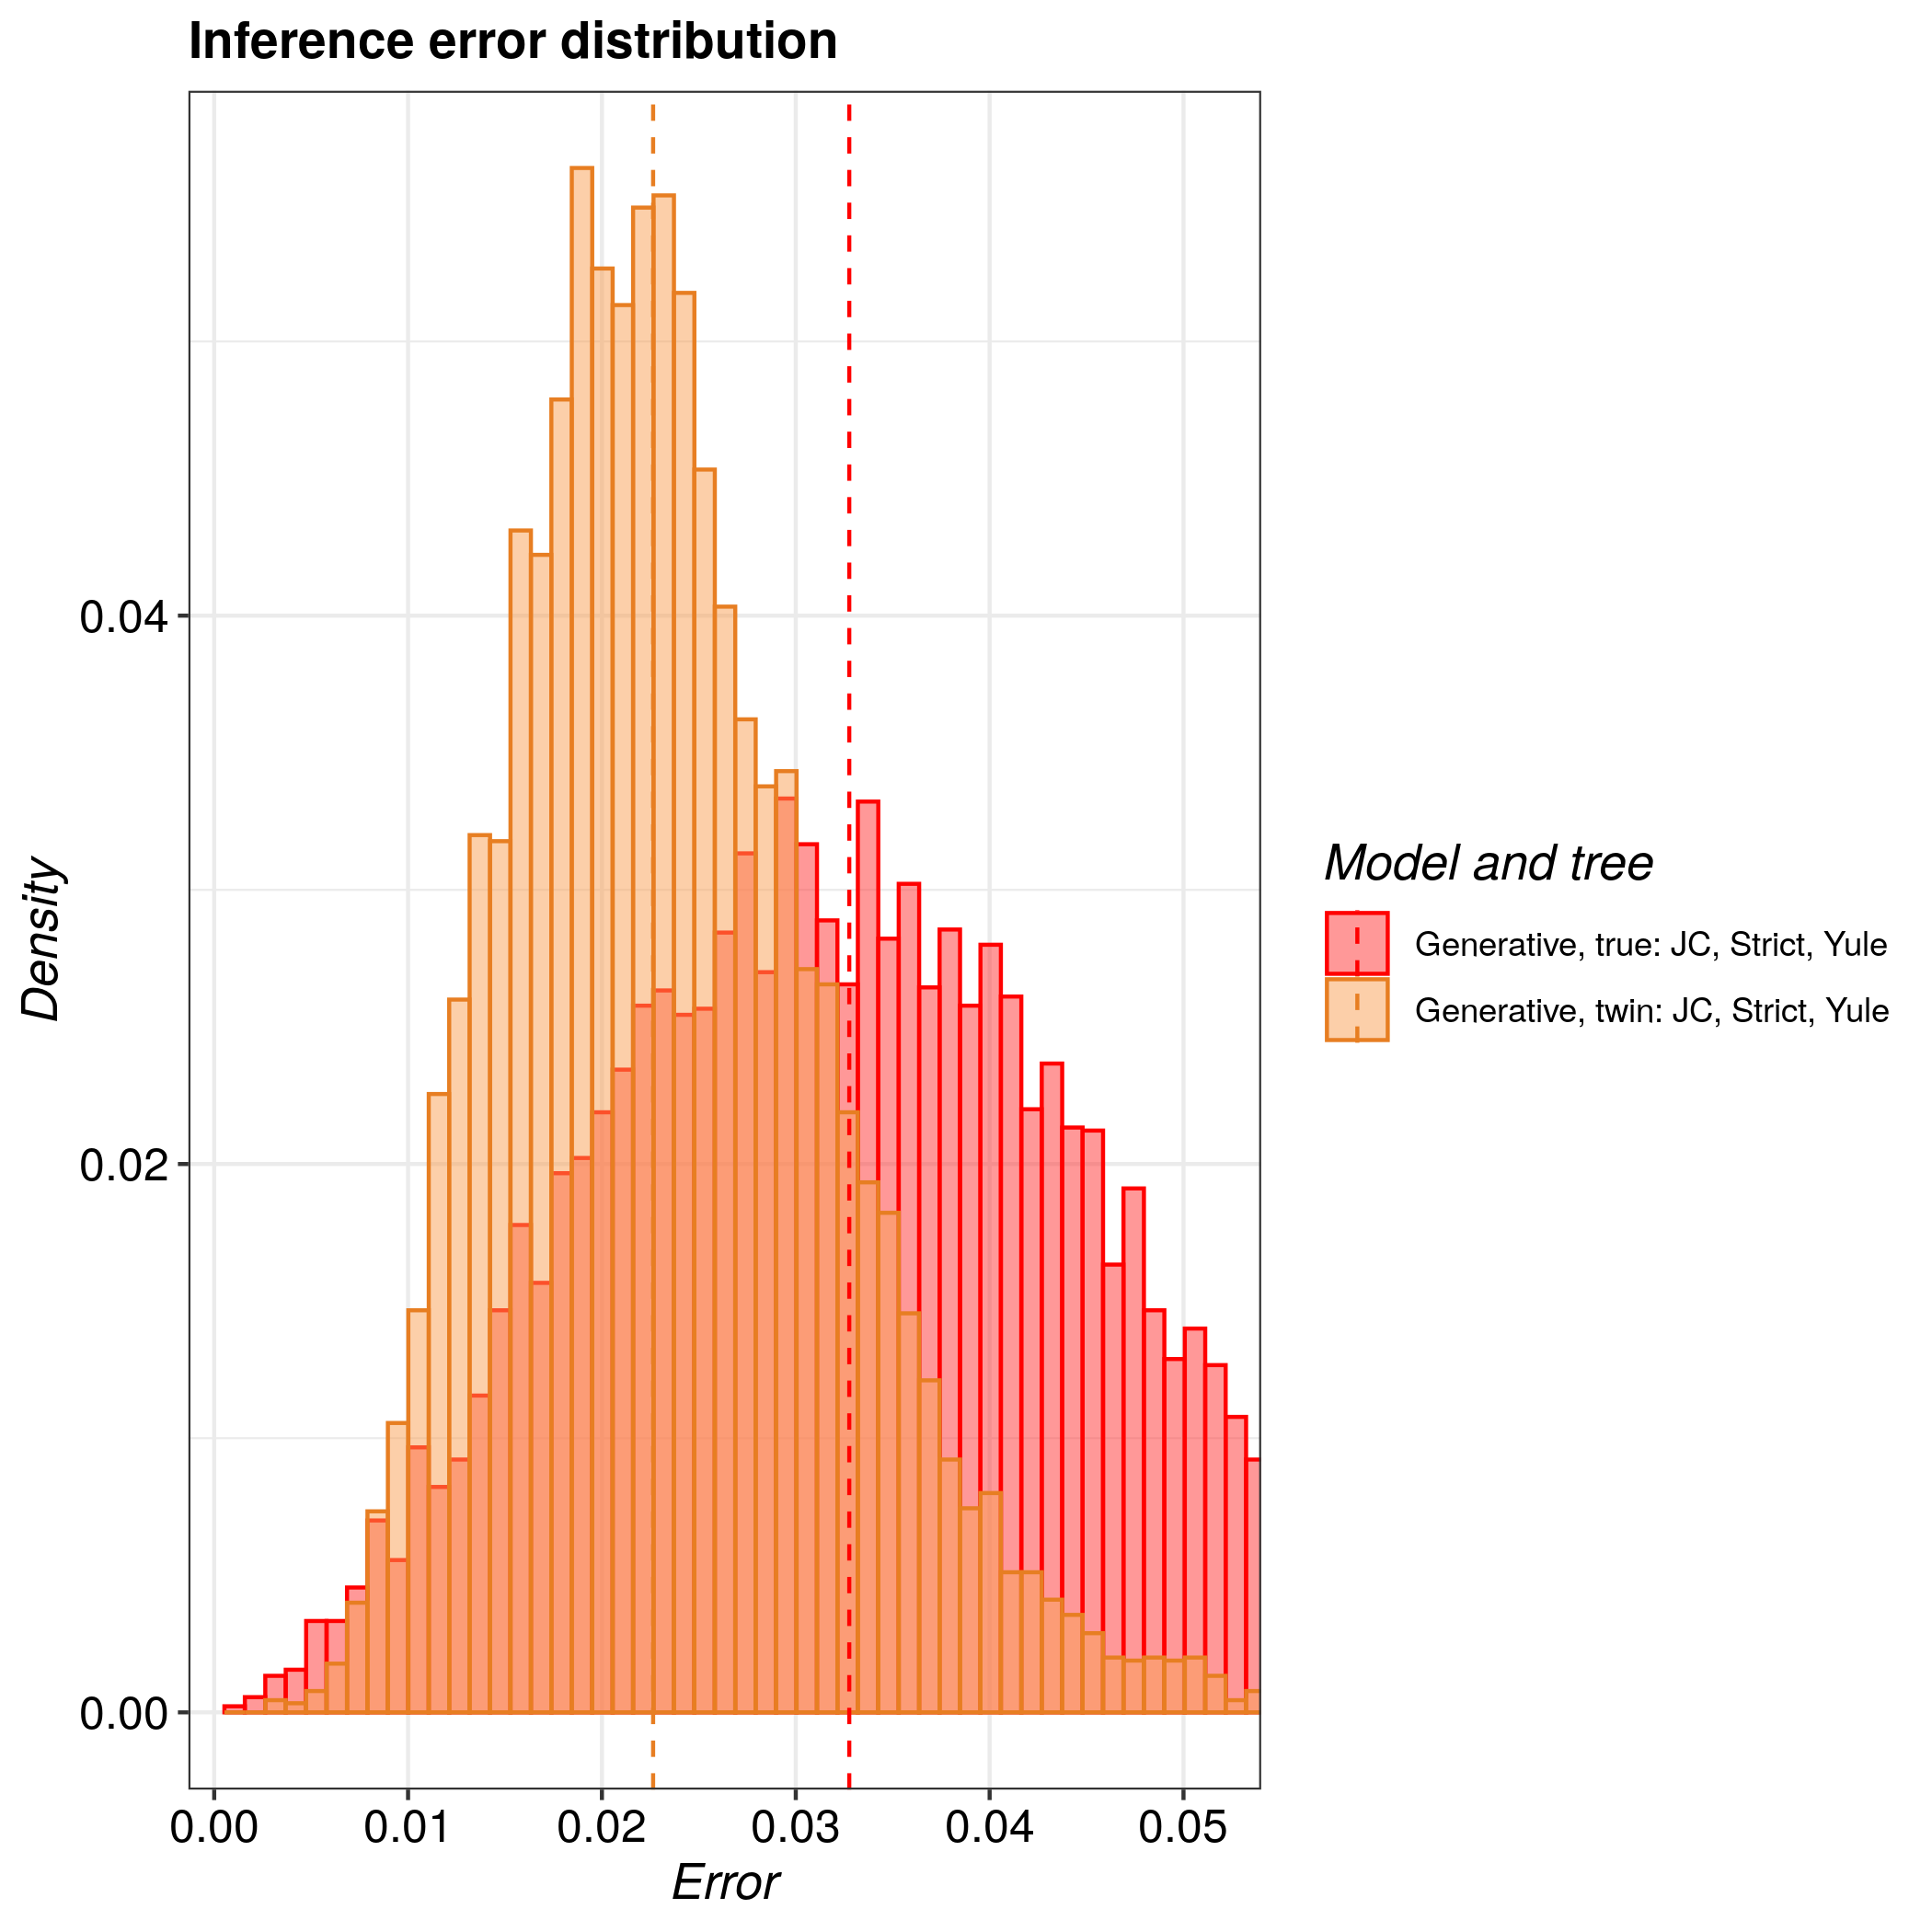
\includegraphics[width=\textwidth]{pirouette_example_22/example_22_314/errors.png}
  \caption{Assuming a Yule tree prior on a Yule tree}
\end{figure}

%%%%%%%%%%%%%%%%%%%%%%%%%%%%%%%%%%%%%%%%%%%%%%%%%%%%%%%%%%%%%%%%%%%%%%%%%%%%%%%%
\subsection{The effect of assuming a Yule tree prior on a BD tree}
%%%%%%%%%%%%%%%%%%%%%%%%%%%%%%%%%%%%%%%%%%%%%%%%%%%%%%%%%%%%%%%%%%%%%%%%%%%%%%%%

The code used in this part of the article can be found at 
\url{https://github.com/richelbilderbeek/pirouette_example_26}.

\richel{depends on https://github.com/richelbilderbeek/pirouette/issues/378}

% \begin{figure}[H]
%   \includegraphics[width=\textwidth]{pirouette_example_26/example_26_314/errors.png}
%   \caption{Assuming a Yule tree prior on a BD tree}
% \end{figure}

%%%%%%%%%%%%%%%%%%%%%%%%%%%%%%%%%%%%%%%%%%%%%%%%%%%%%%%%%%%%%%%%%%%%%%%%%%%%%%%%
\subsection{The effect of differently common diversity-dependent trees}
%%%%%%%%%%%%%%%%%%%%%%%%%%%%%%%%%%%%%%%%%%%%%%%%%%%%%%%%%%%%%%%%%%%%%%%%%%%%%%%%

Here we show the results of a \verb;pirouette; run on a dataset of $N = 100$ \giovanni{N can be changed if 100 is too much} trees simulated under a diversity-dependent process. All the trees are simulated using the DDD package (\cite{DDD}). Our goal is to show how trees simulated by a process that is sensibly different from a standard tree prior will result in a significant divergence between true and twin distribution. To do so we set the simulation parameters (in this case: absolute speciation rate $\lambda_0 = 1.6$, extinction rate $\mu = 0.2$ and carrying capacity $K = 20$) in order to express clear characteristics of diversity dependence in the phylogenies. In fact, for a high speciation rate and a low carrying capacity we expect trees to exhibit high unbalance, compared with trees generated by a standard birth-death model. We can measure how unbalanced is a tree using the $\gamma$ statistics (\cite{pybus2000testing}). For this reason, we choose to measure the error made by the inference process using the $\gamma$ error statistics, which is currently implemented in \verb;pirouette;.

The code used in this part of the article can be found at 
\url{https://github.com/richelbilderbeek/pirouette_example_23}.

\begin{figure}[H]
  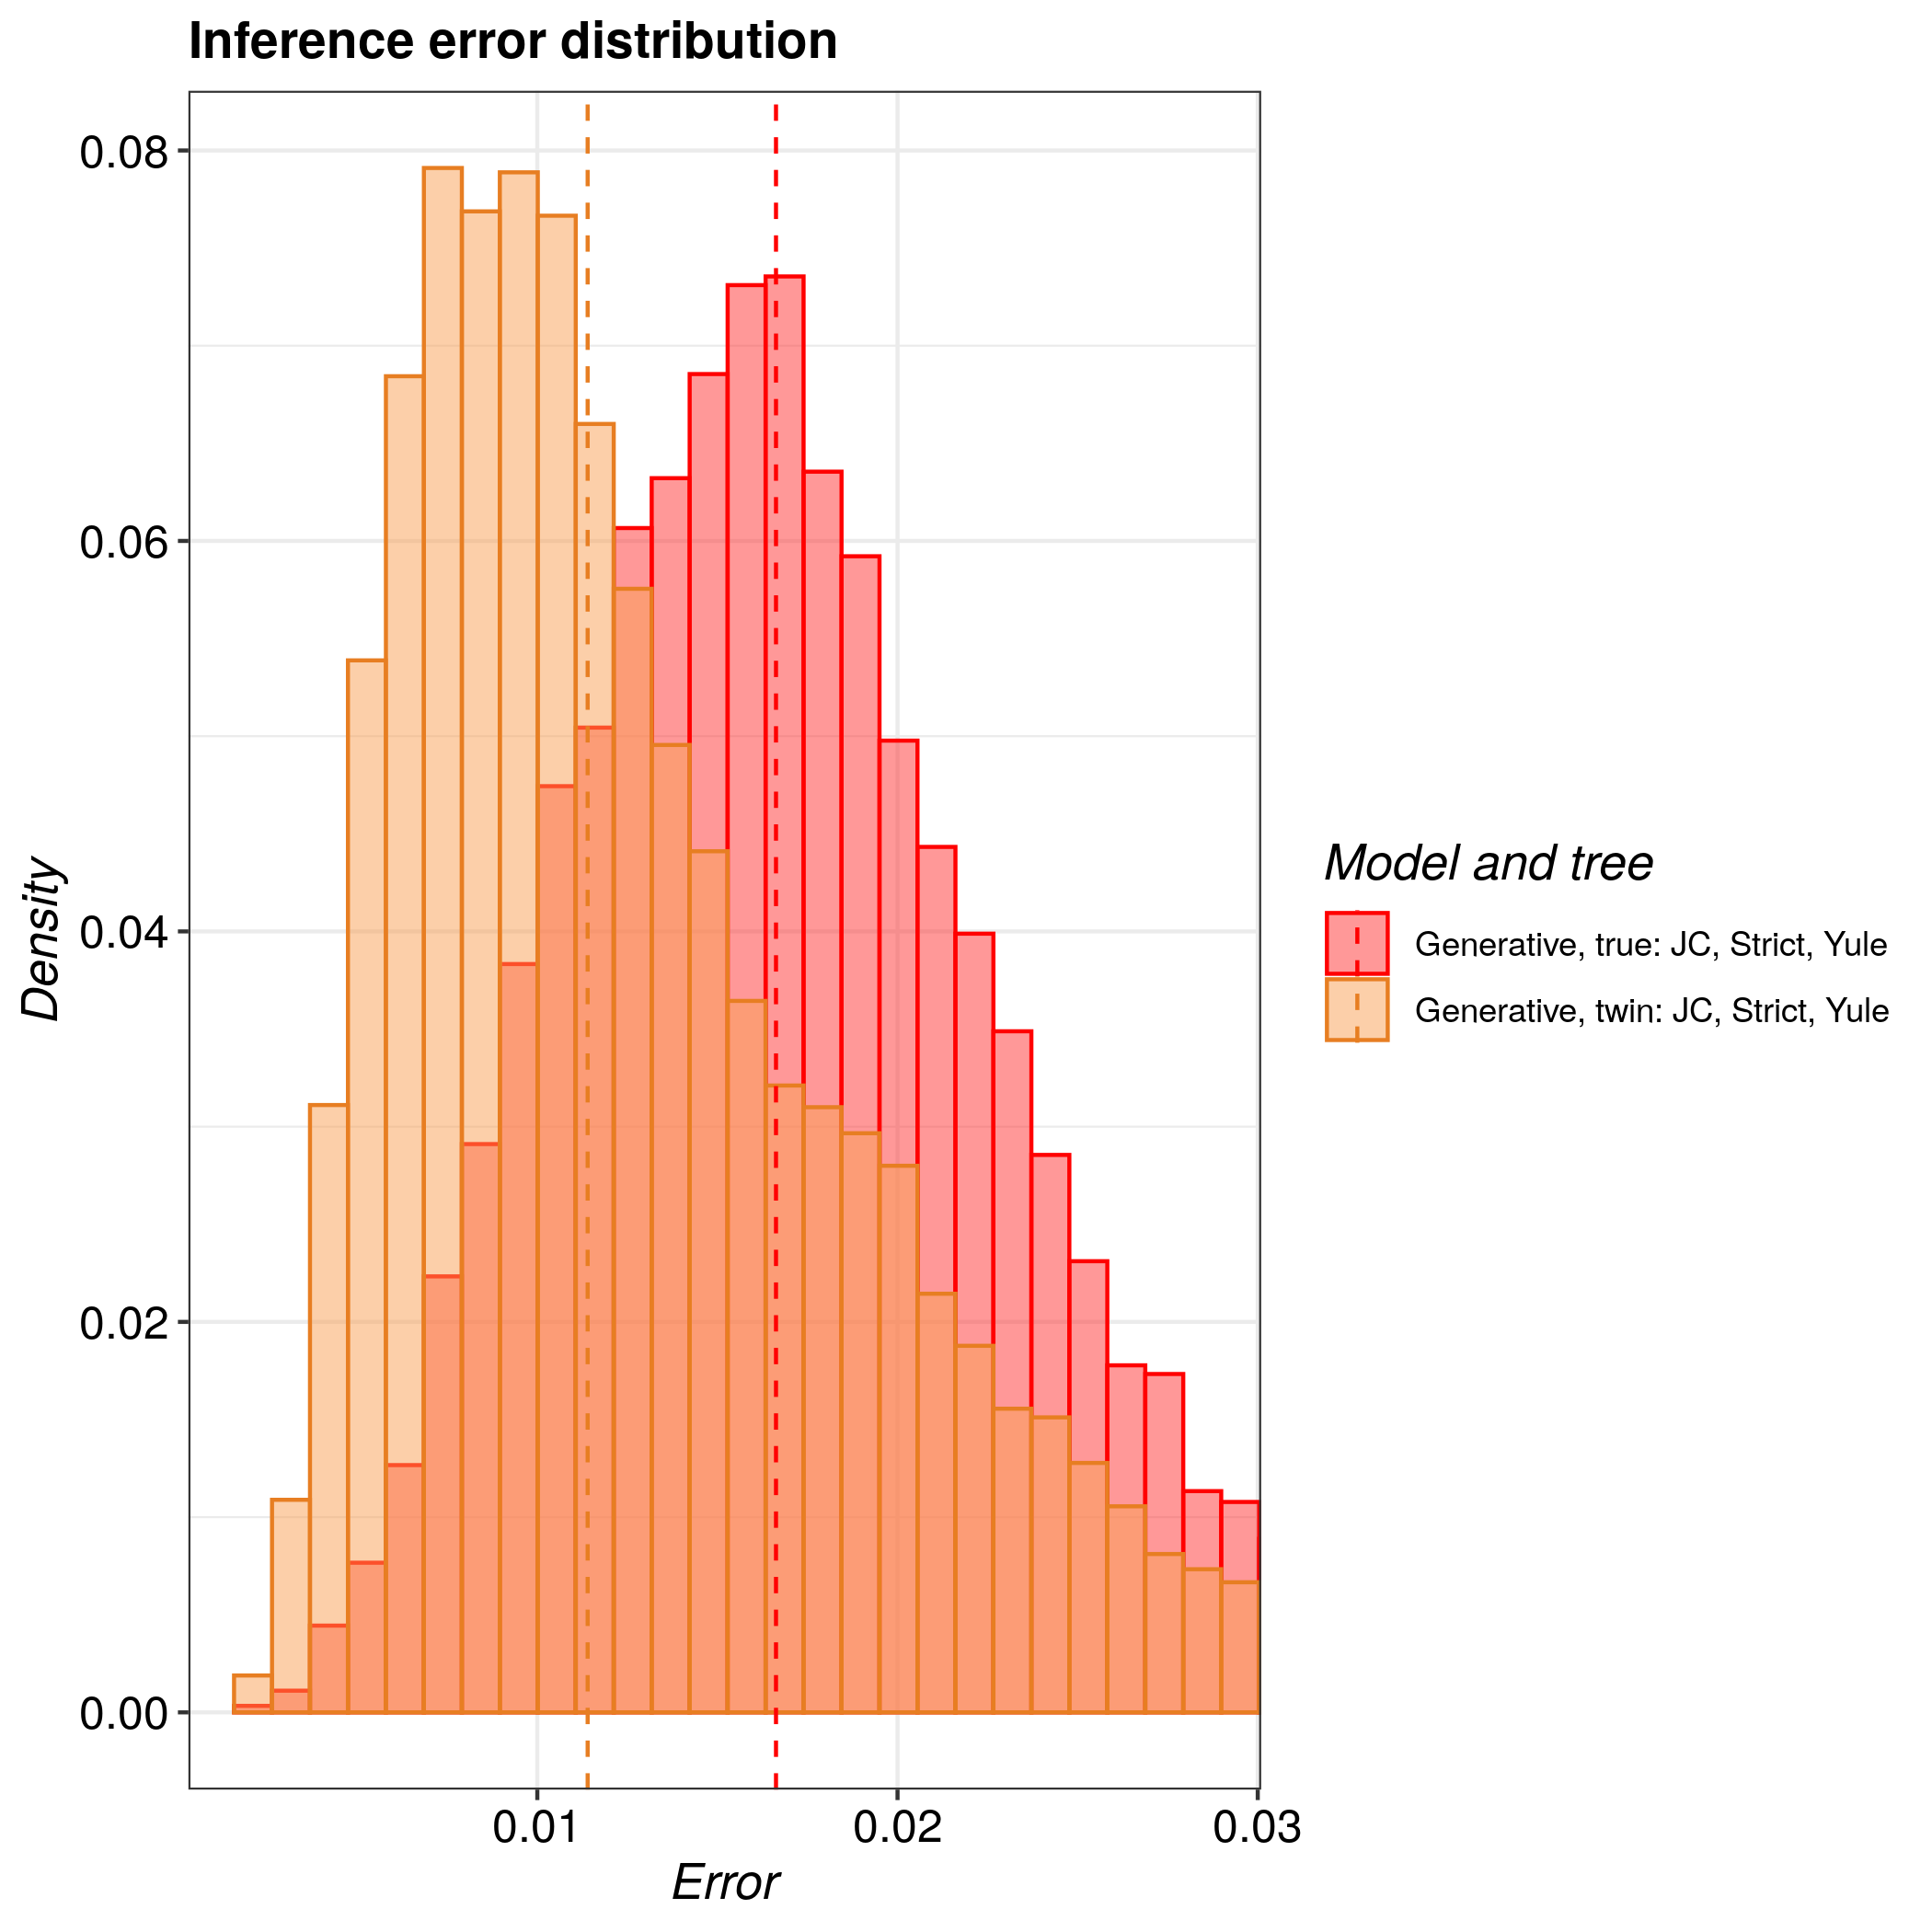
\includegraphics[width=\textwidth]{pirouette_example_23/example_23_314/errors.png}
  \caption{Lowest likelihood}
\end{figure}

\begin{figure}[H]
  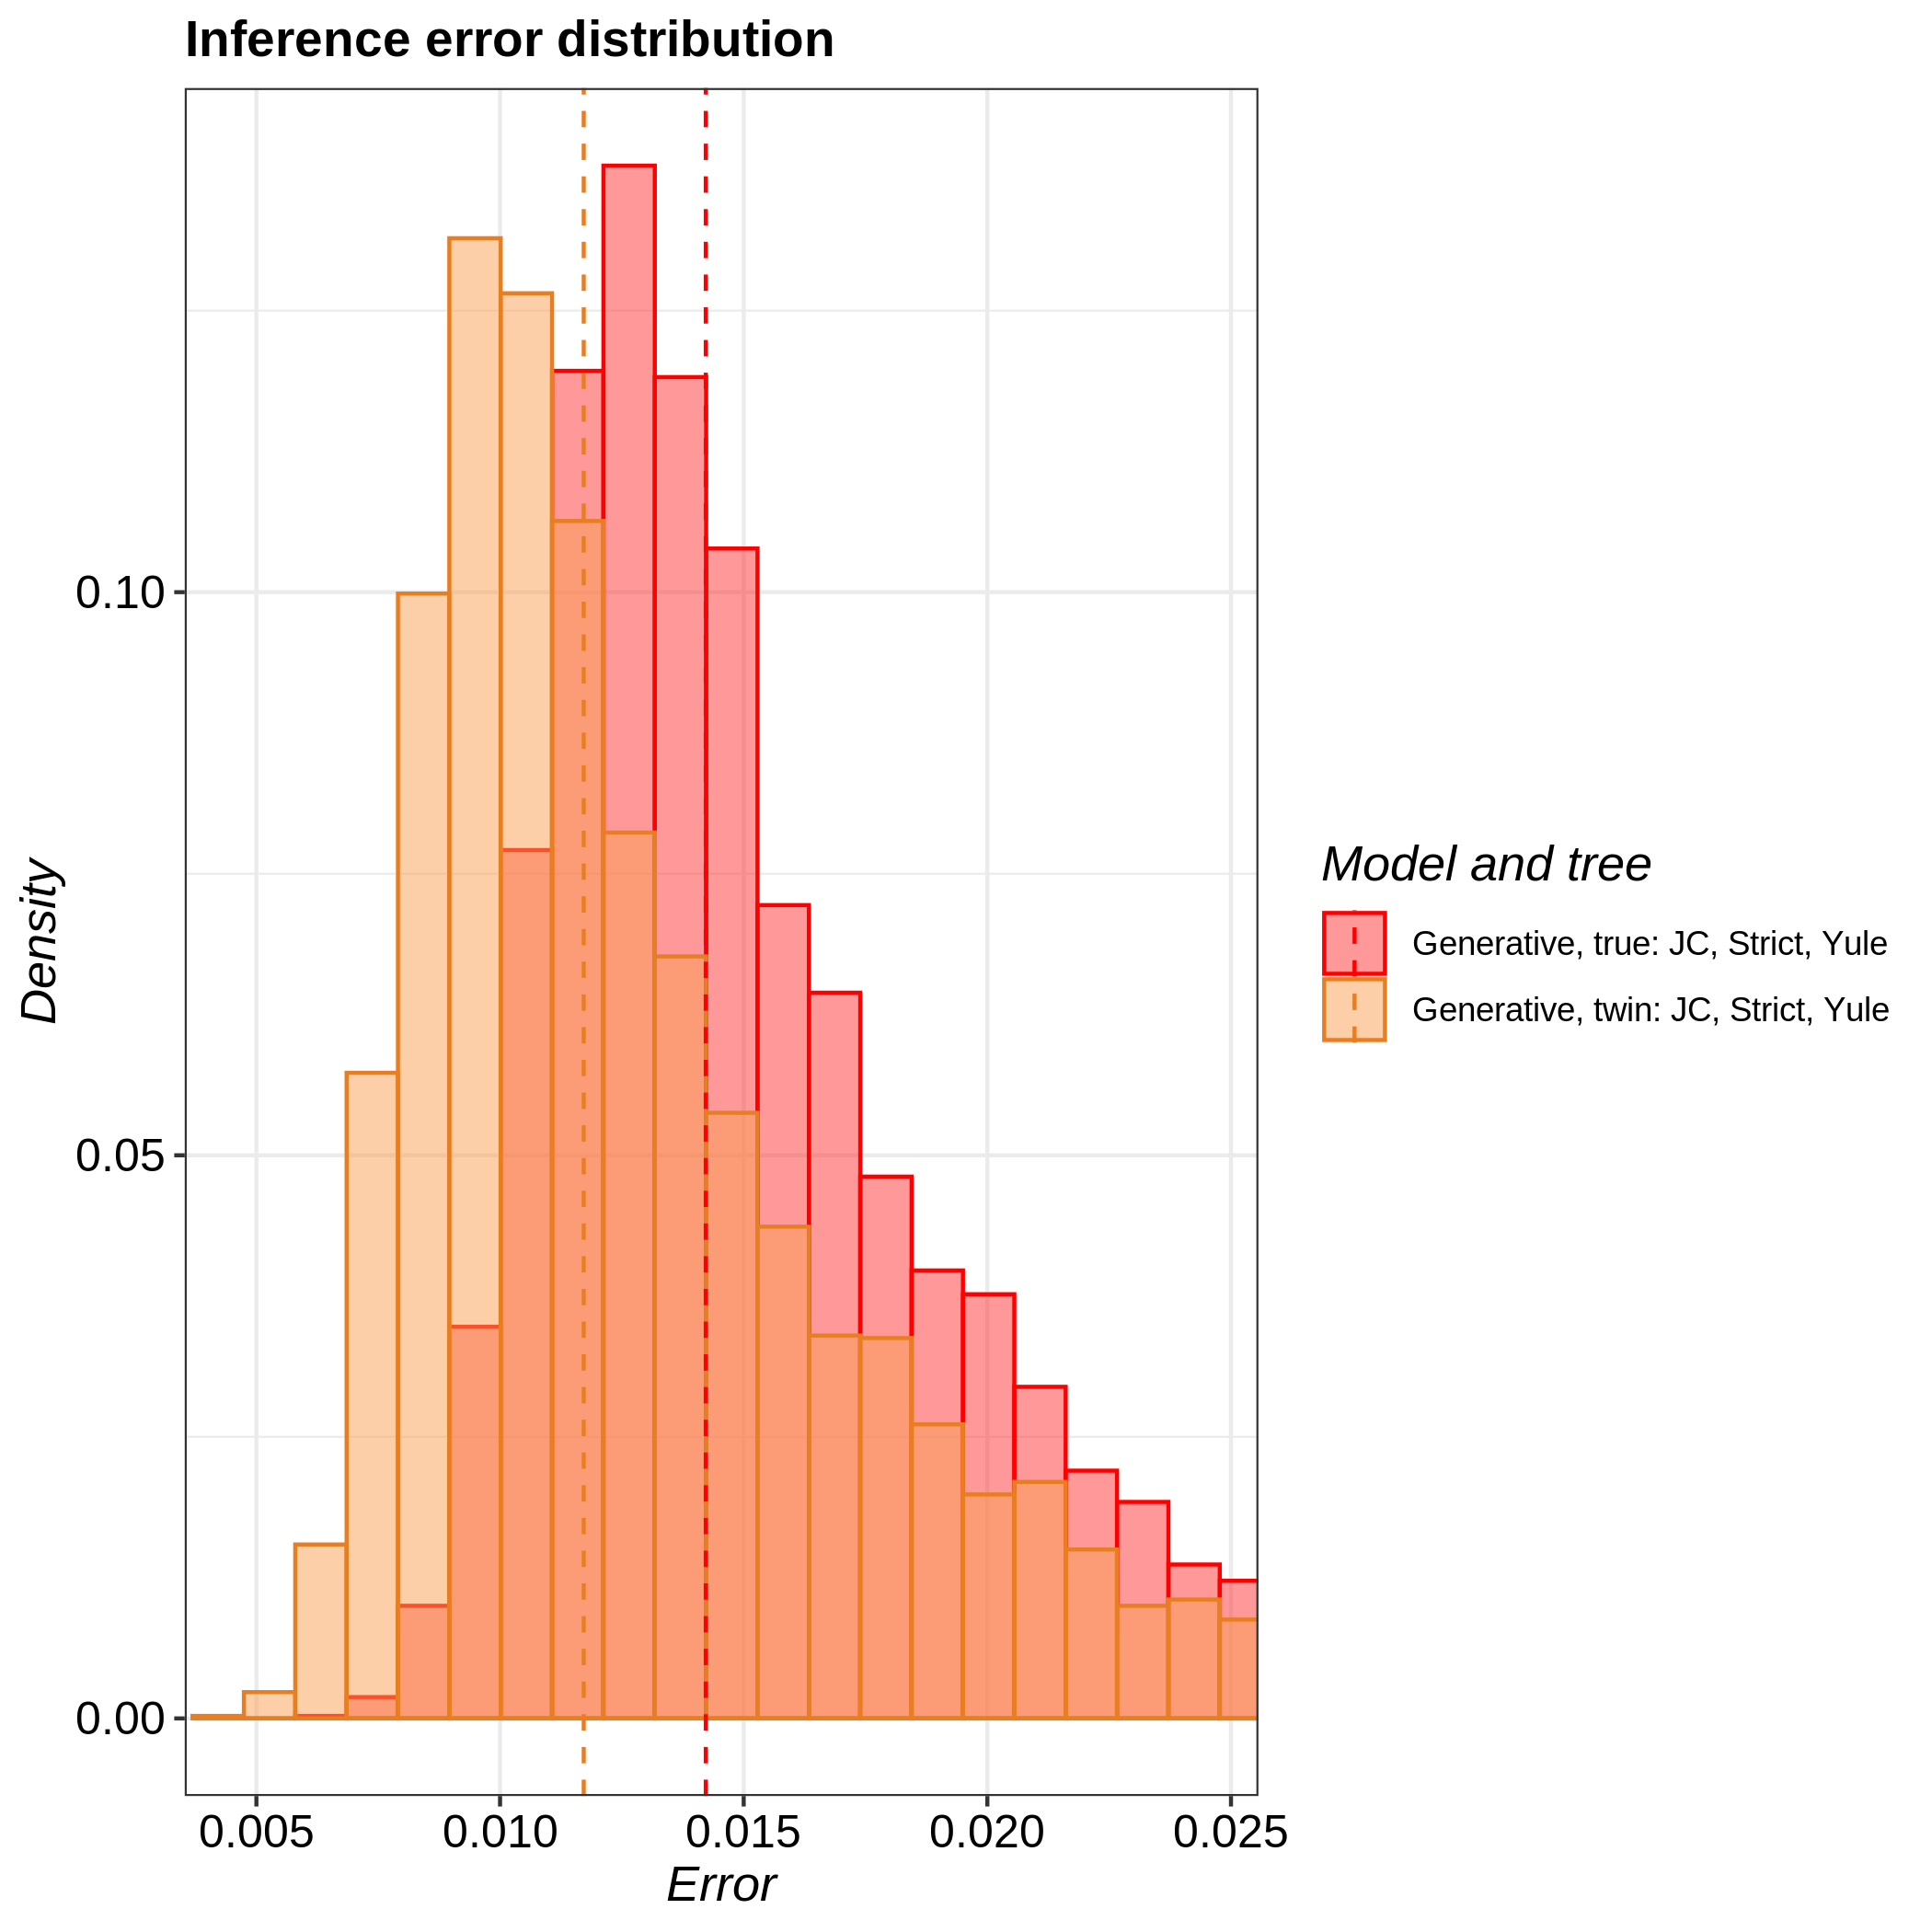
\includegraphics[width=\textwidth]{pirouette_example_23/example_23_315/errors.png}
  \caption{Between lowest and median likelihood}
\end{figure}

\begin{figure}[H]
  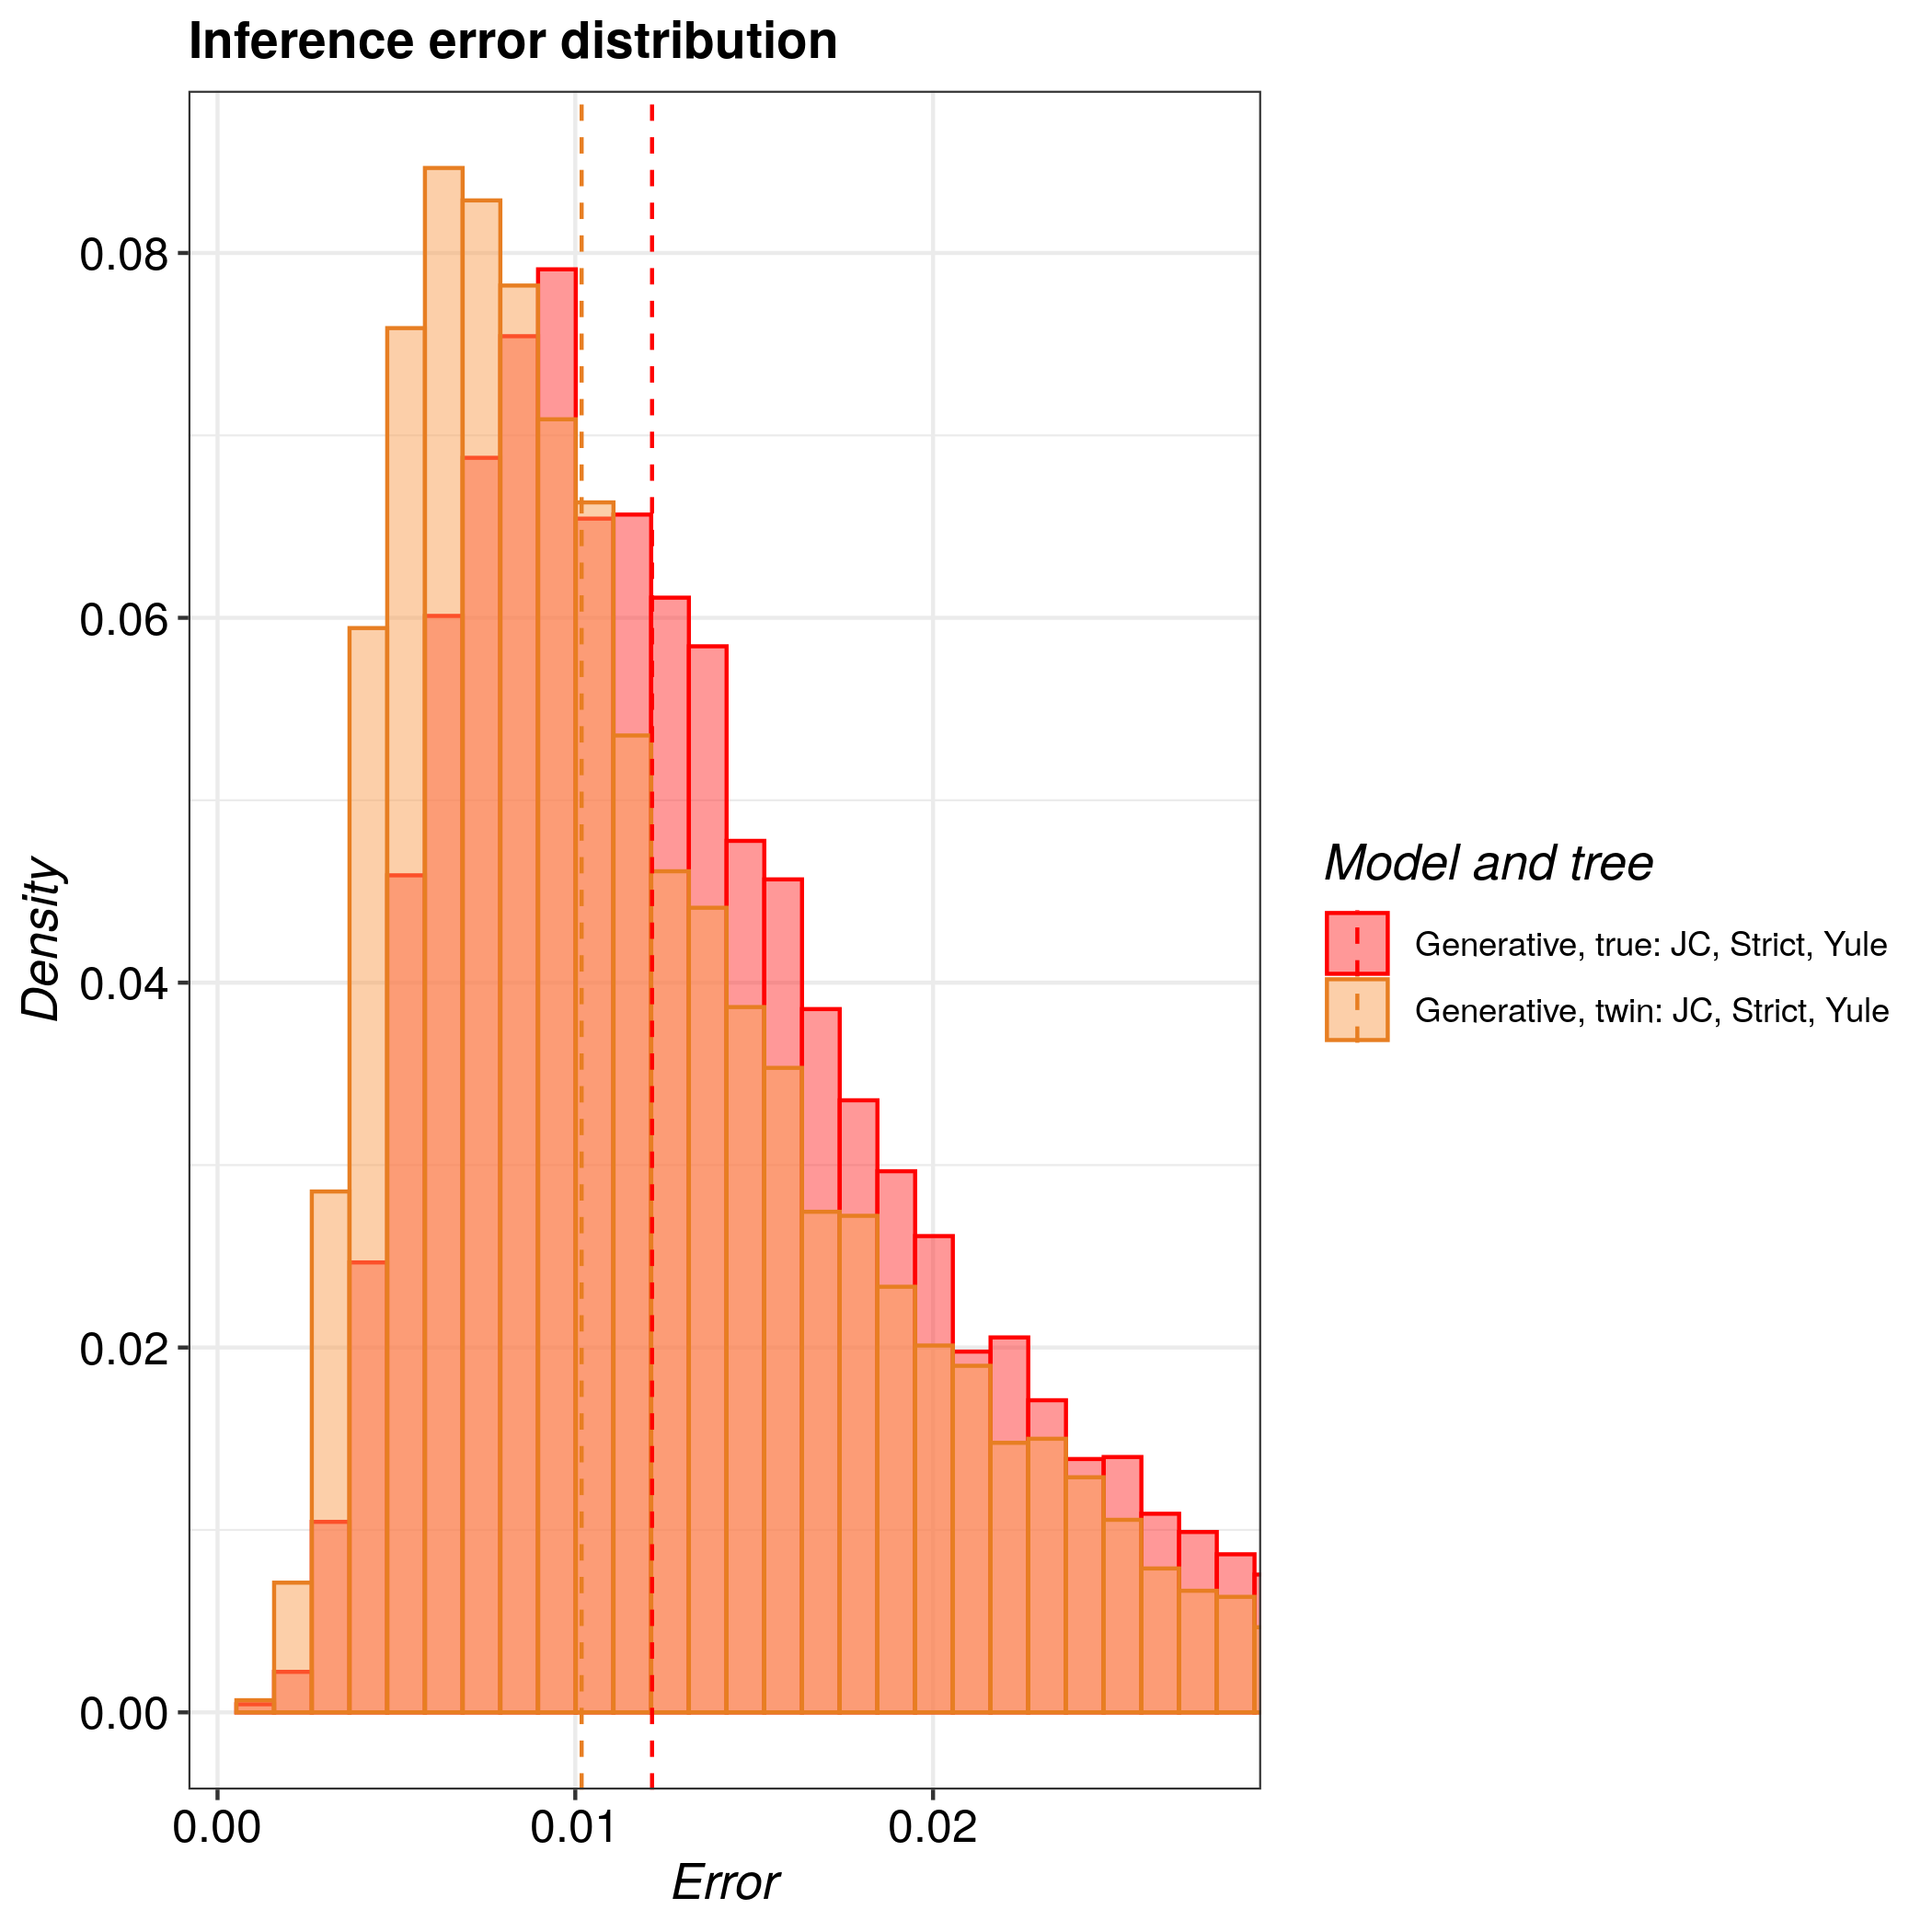
\includegraphics[width=\textwidth]{pirouette_example_23/example_23_316/errors.png}
  \caption{Median likelihood}
\end{figure}


\begin{figure}[H]
  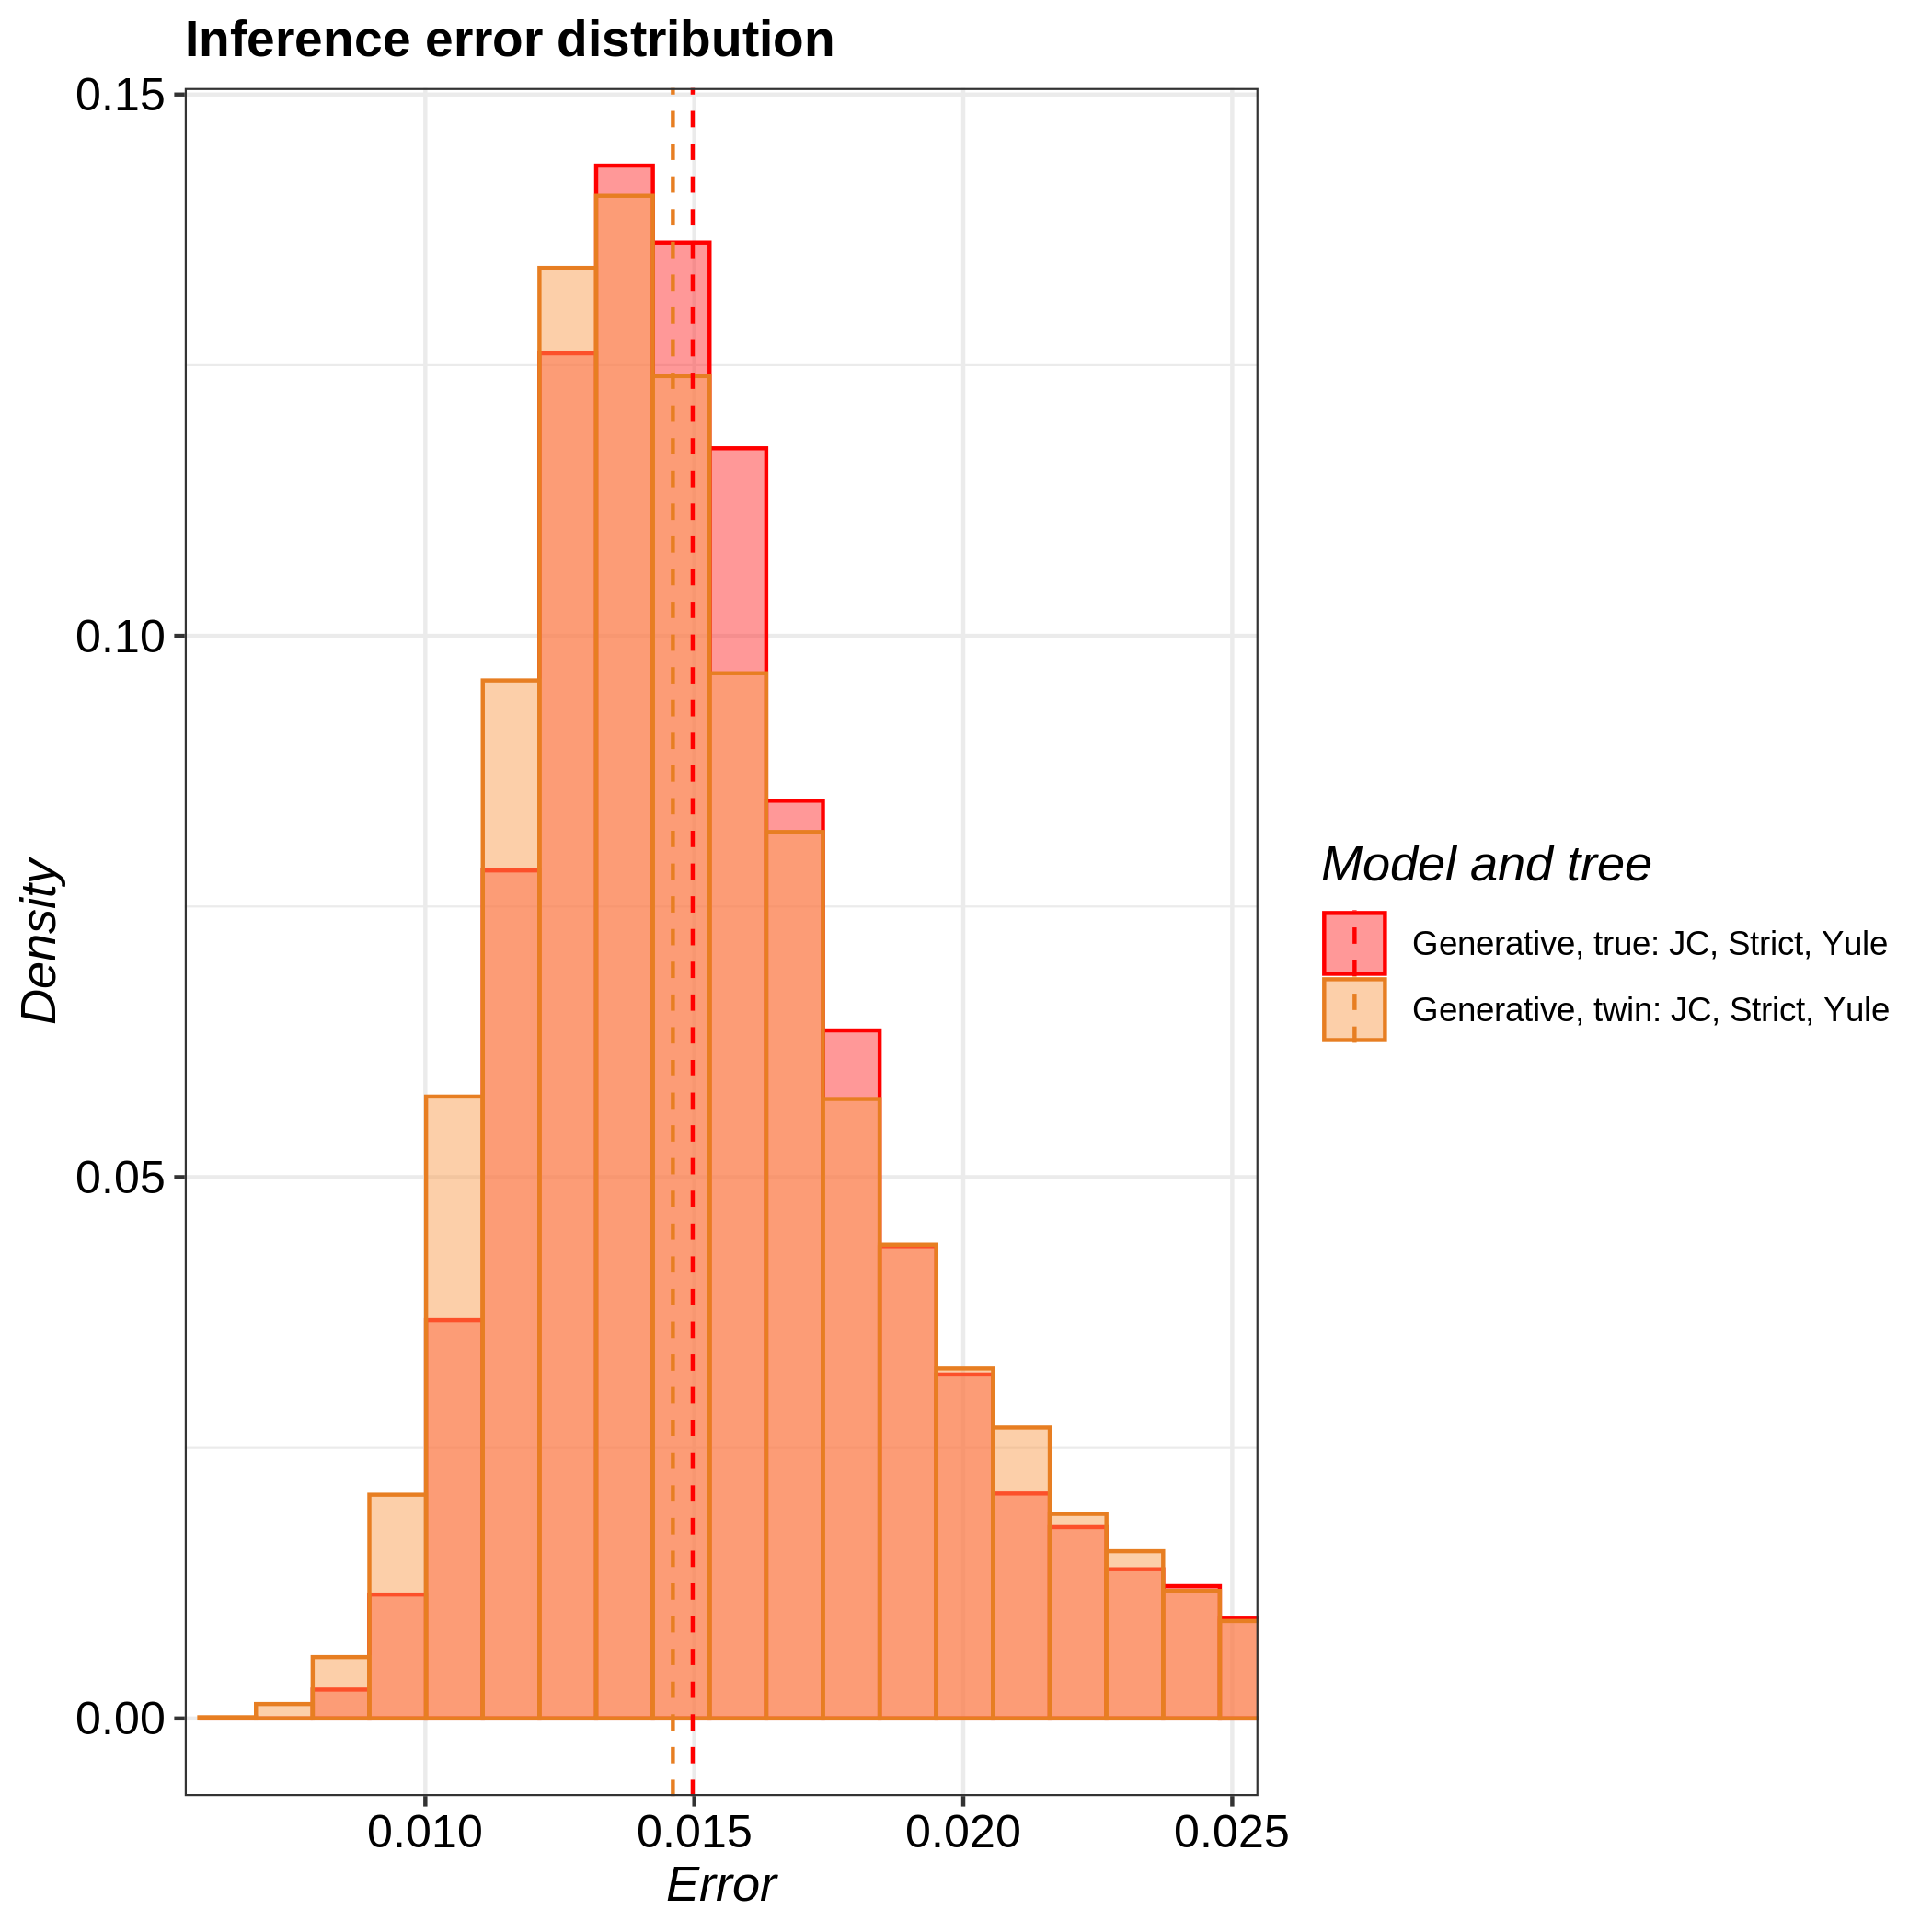
\includegraphics[width=\textwidth]{pirouette_example_23/example_23_317/errors.png}
  \caption{Between median and highest likelihood}
\end{figure}

\begin{figure}[H]
  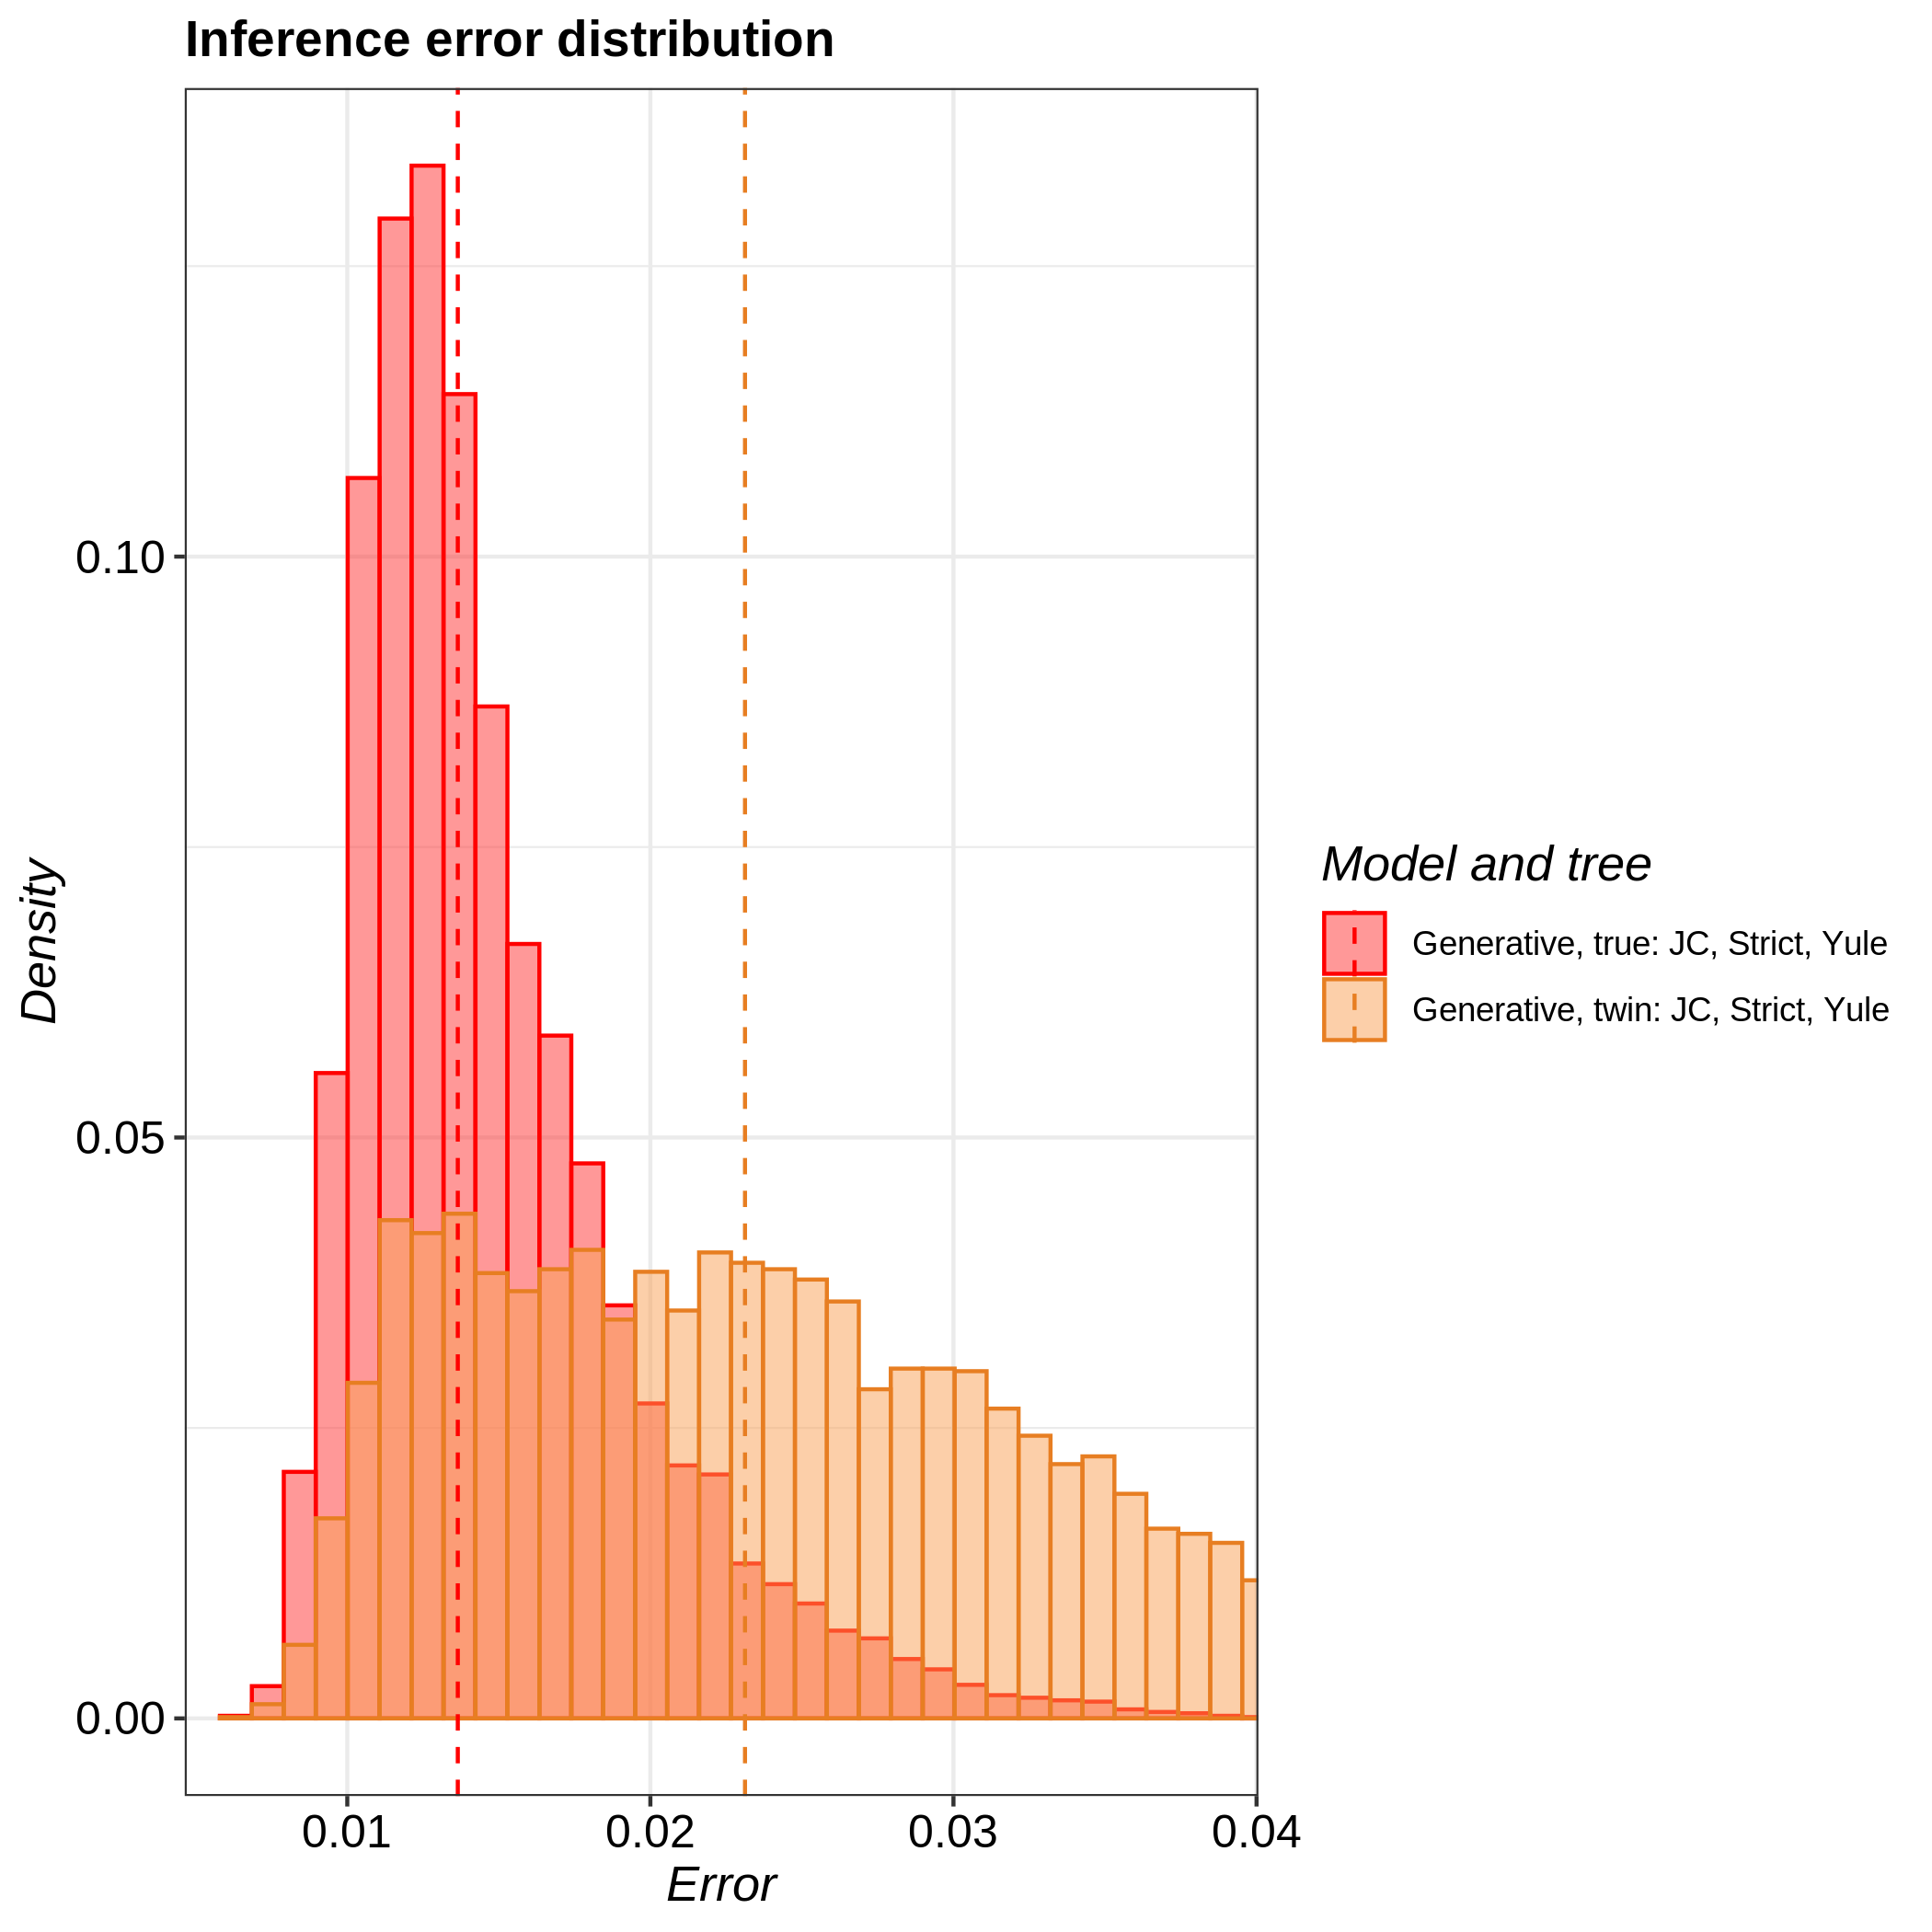
\includegraphics[width=\textwidth]{pirouette_example_23/example_23_318/errors.png}
  \caption{Highest likelihood}
\end{figure}

%%%%%%%%%%%%%%%%%%%%%%%%%%%%%%%%%%%%%%%%%%%%%%%%%%%%%%%%%%%%%%%%%%%%%%%%%%%%%%%%
\subsection{The effect of equal or equalized mutation rate in the twin alignment}
%%%%%%%%%%%%%%%%%%%%%%%%%%%%%%%%%%%%%%%%%%%%%%%%%%%%%%%%%%%%%%%%%%%%%%%%%%%%%%%%

\begin{figure}[H]
  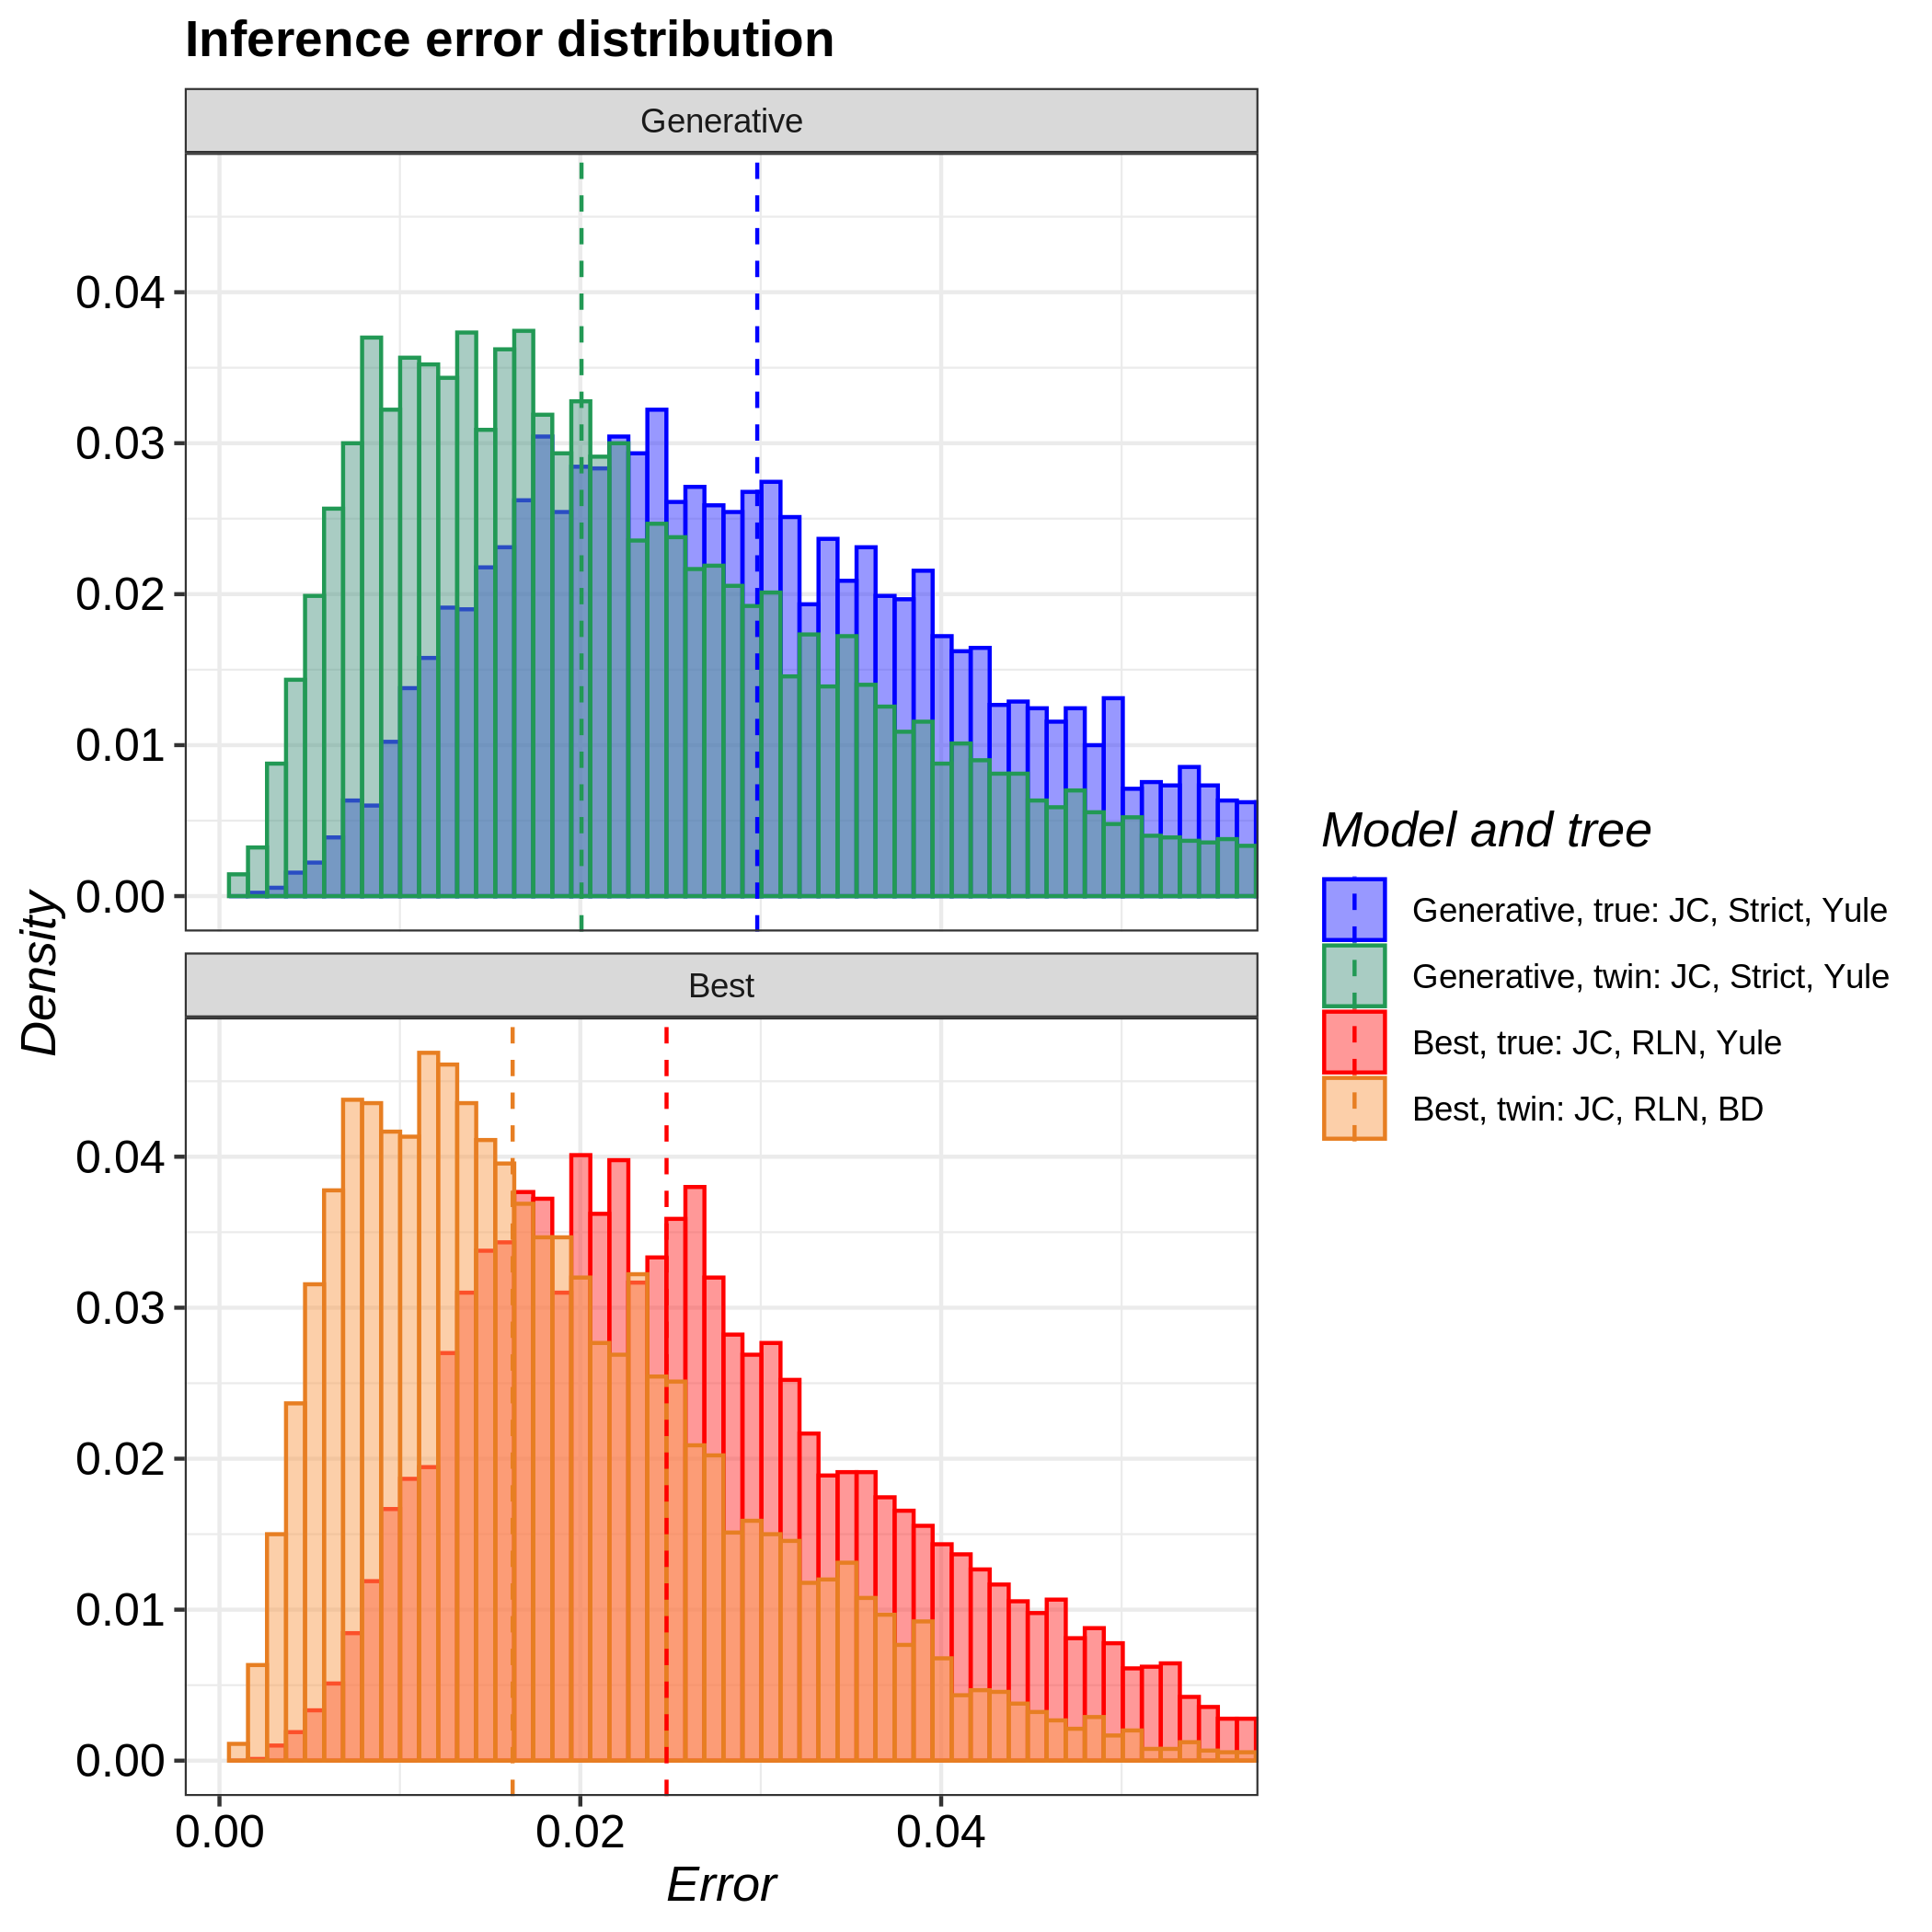
\includegraphics[width=\textwidth]{pirouette_example_30/example_30_314/errors.png}
  \caption{Equal number of mutations}
\end{figure}

\begin{figure}[H]
  \includegraphics[width=\textwidth]{pirouette_example_3008/example_18_314/errors.png}
  \caption{Equal mutation rate}
\end{figure}

%%%%%%%%%%%%%%%%%%%%%%%%%%%%%%%%%%%%%%%%%%%%%%%%%%%%%%%%%%%%%%%%%%%%%%%%%%%%%%%%
\subsection{The effect of mutation rate}
%%%%%%%%%%%%%%%%%%%%%%%%%%%%%%%%%%%%%%%%%%%%%%%%%%%%%%%%%%%%%%%%%%%%%%%%%%%%%%%%

The code used in this part of the article can be found at 
\url{https://github.com/richelbilderbeek/pirouette_example_24}.

\begin{figure}[H]
  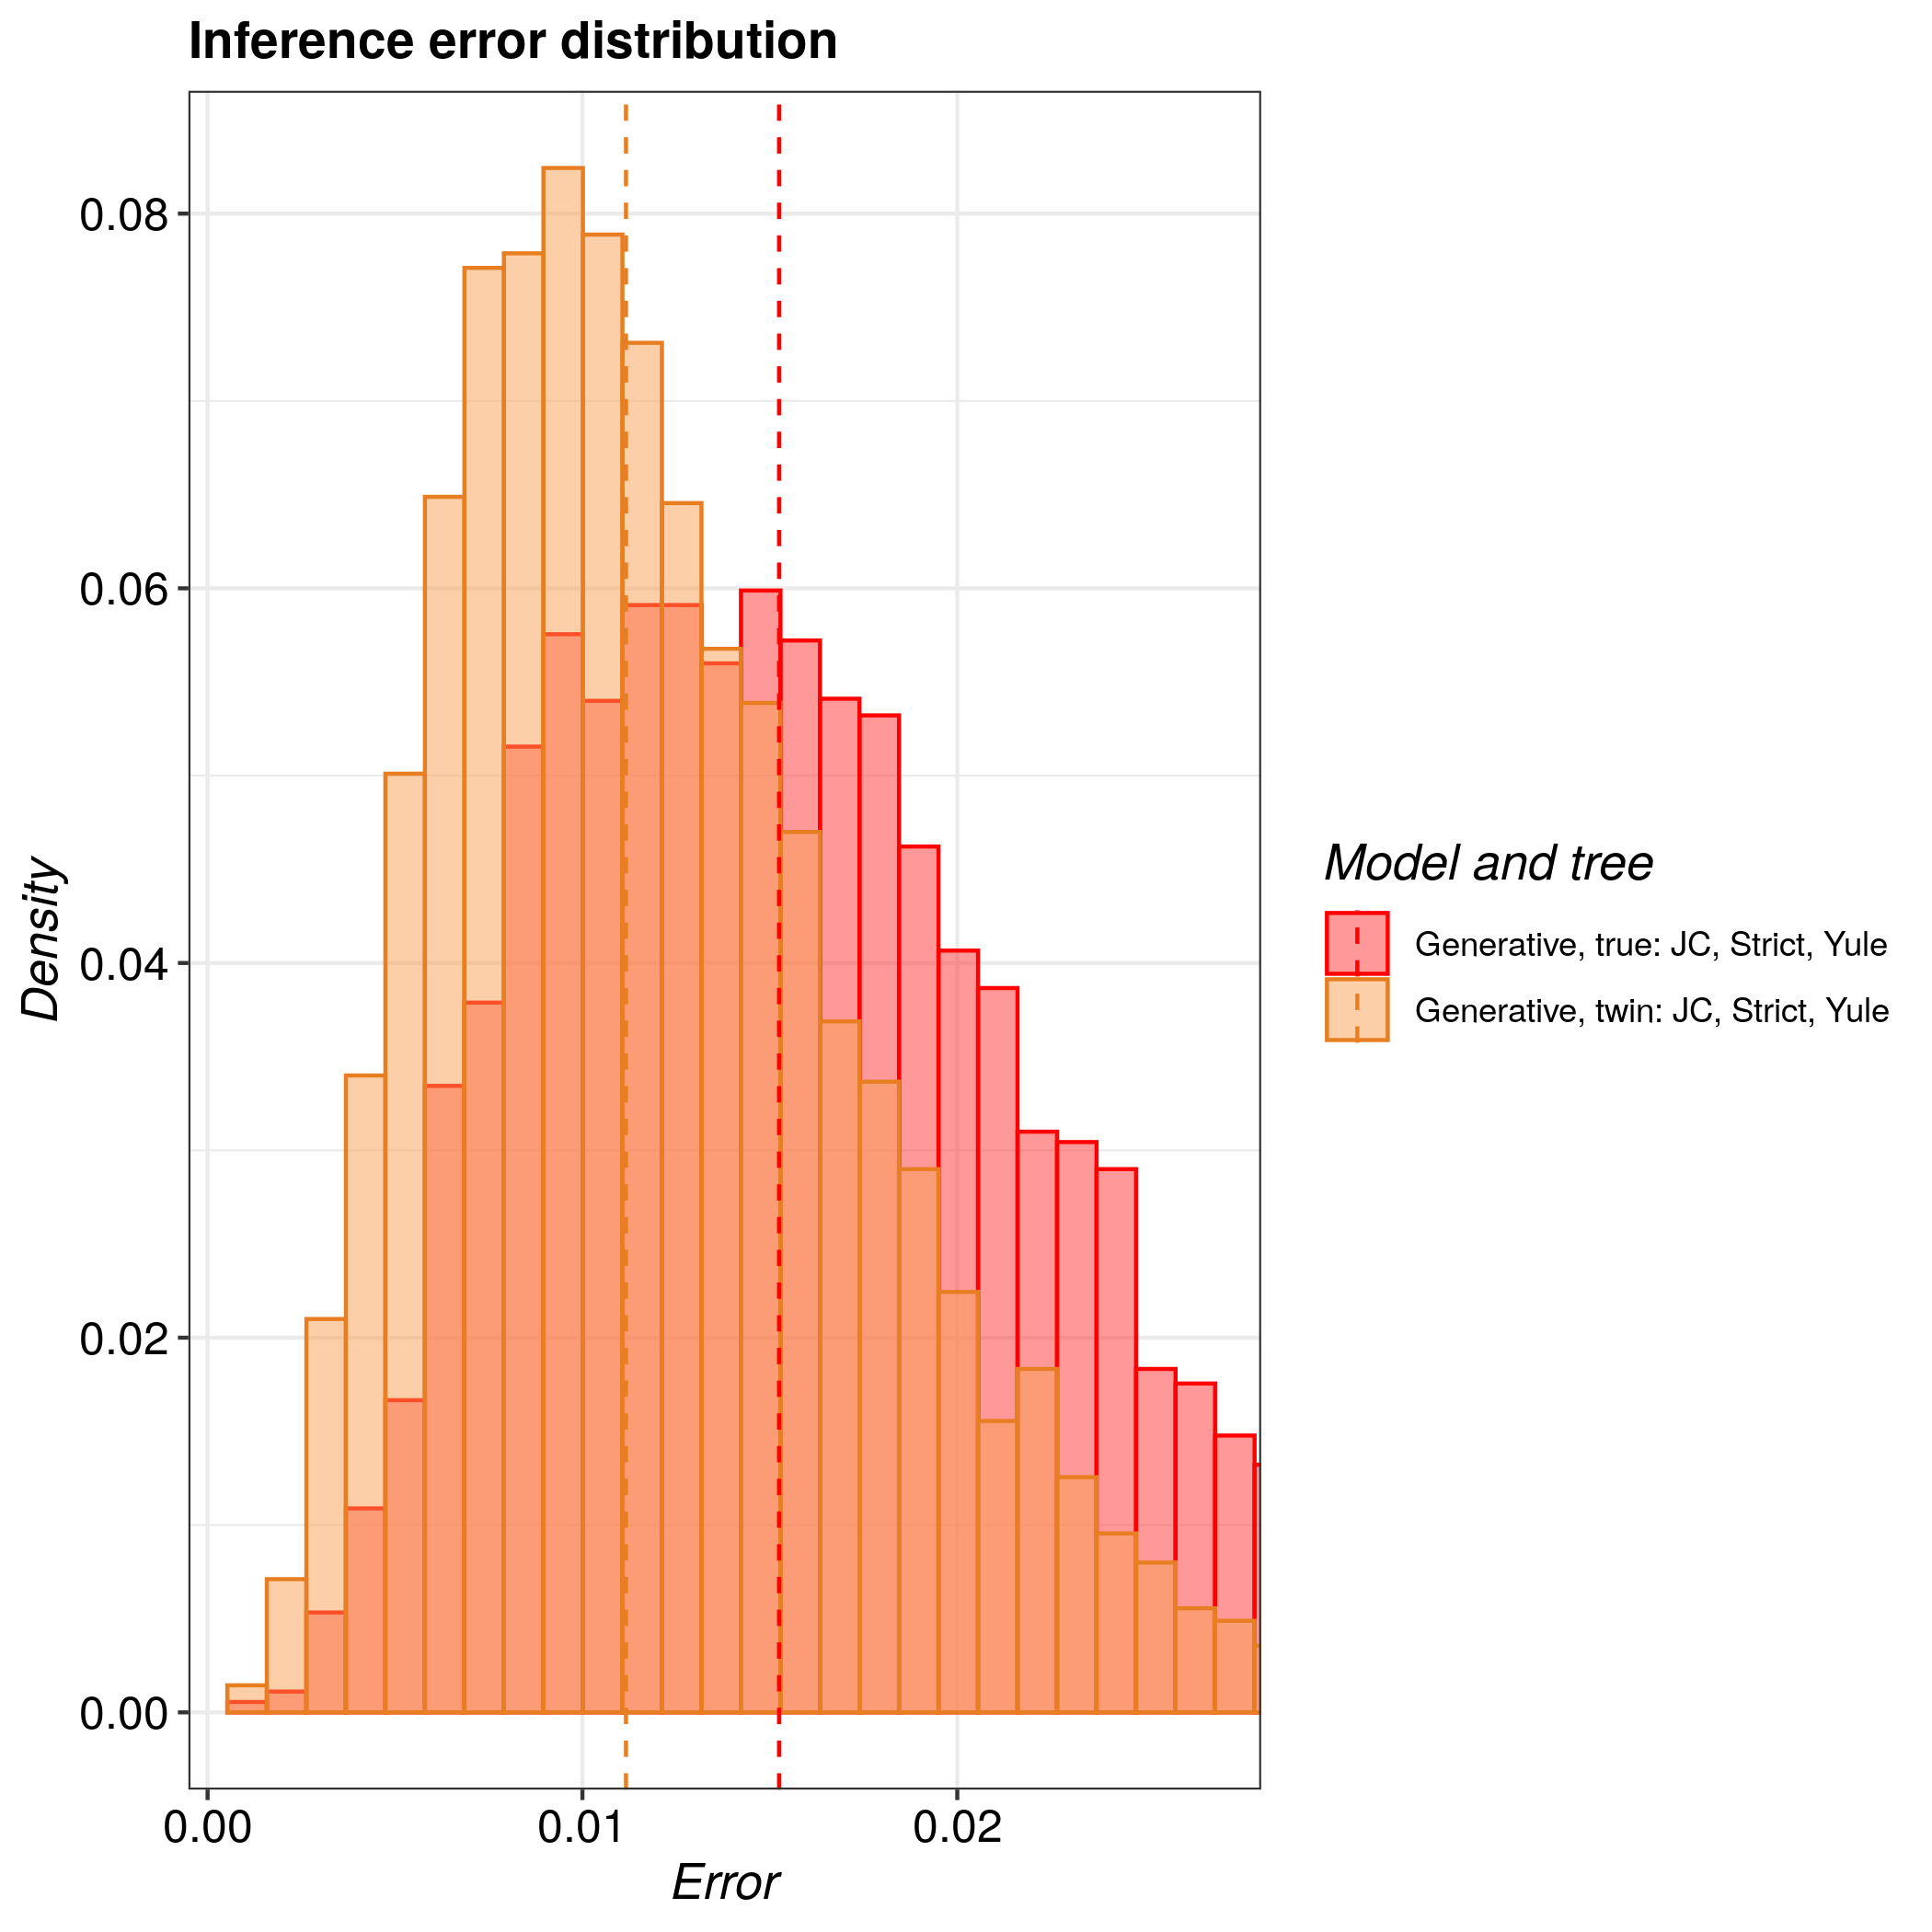
\includegraphics[width=\textwidth]{pirouette_example_24/example_24_314/errors.png}
  \caption{Per-nucleotide mutation rate of 0.0125}
\end{figure}


\begin{figure}[H]
  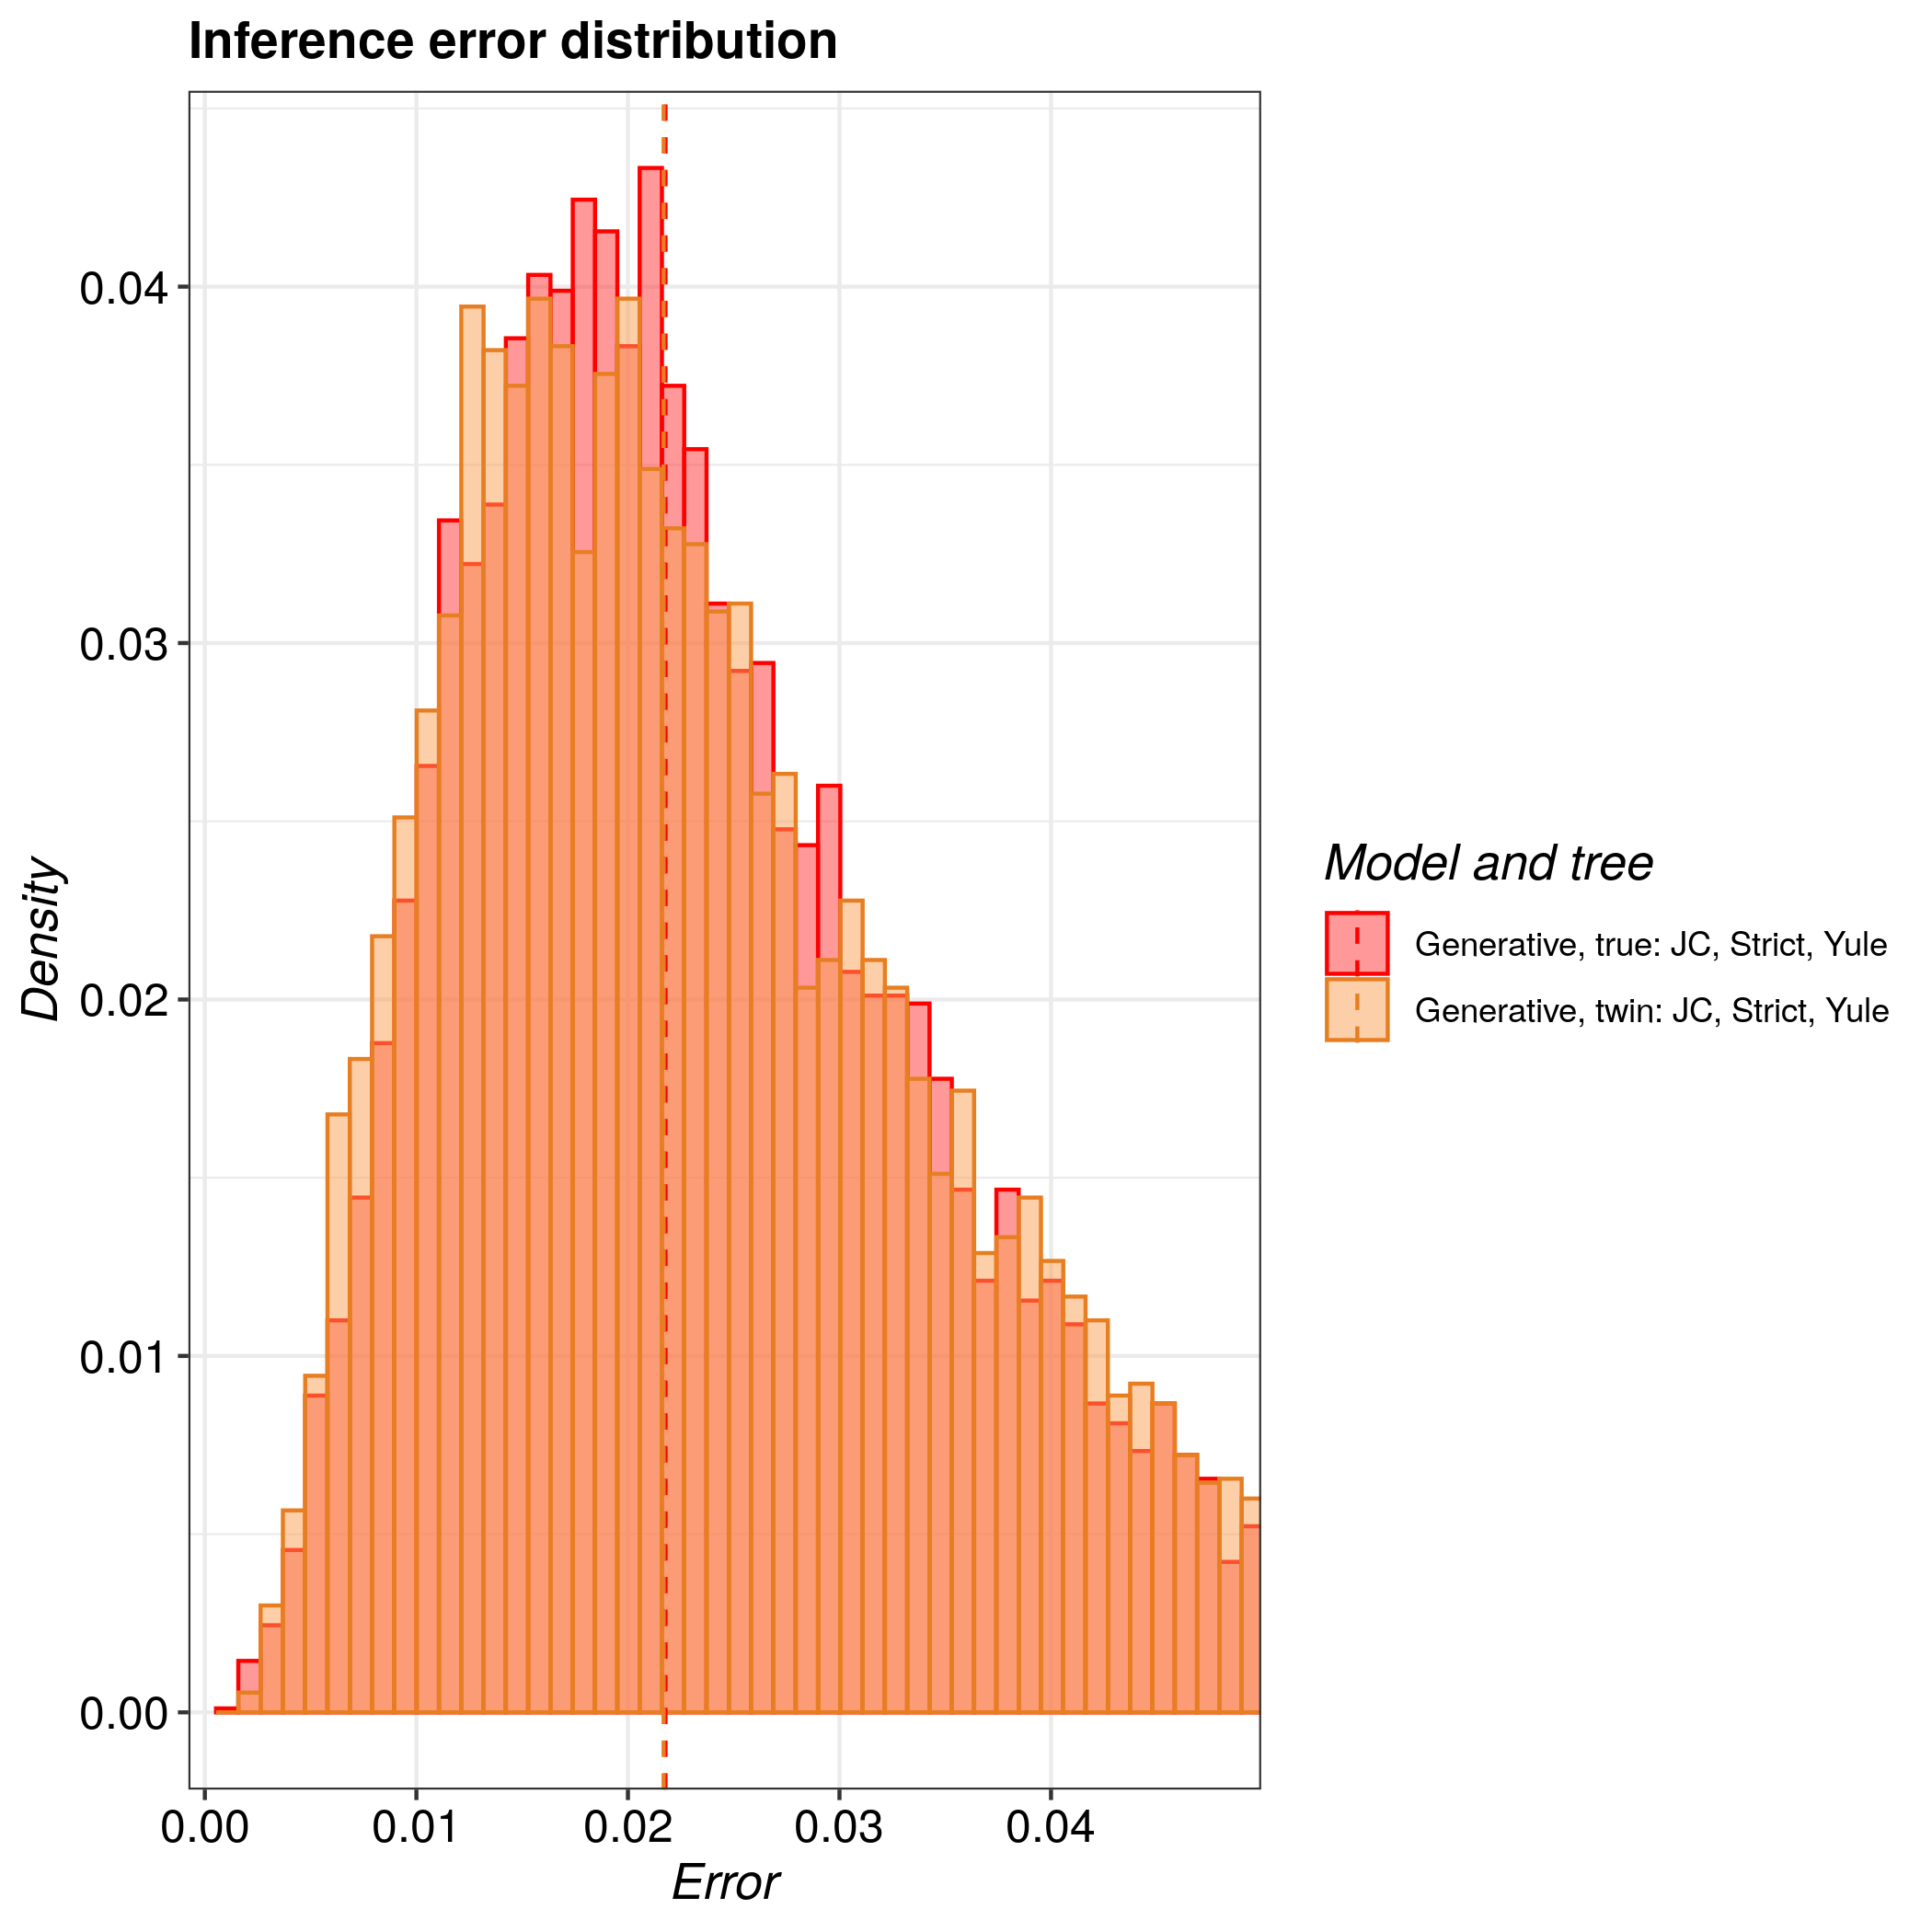
\includegraphics[width=\textwidth]{pirouette_example_24/example_24_315/errors.png}
  \caption{Per-nucleotide mutation rate of 0.025}
\end{figure}

\begin{figure}[H]
  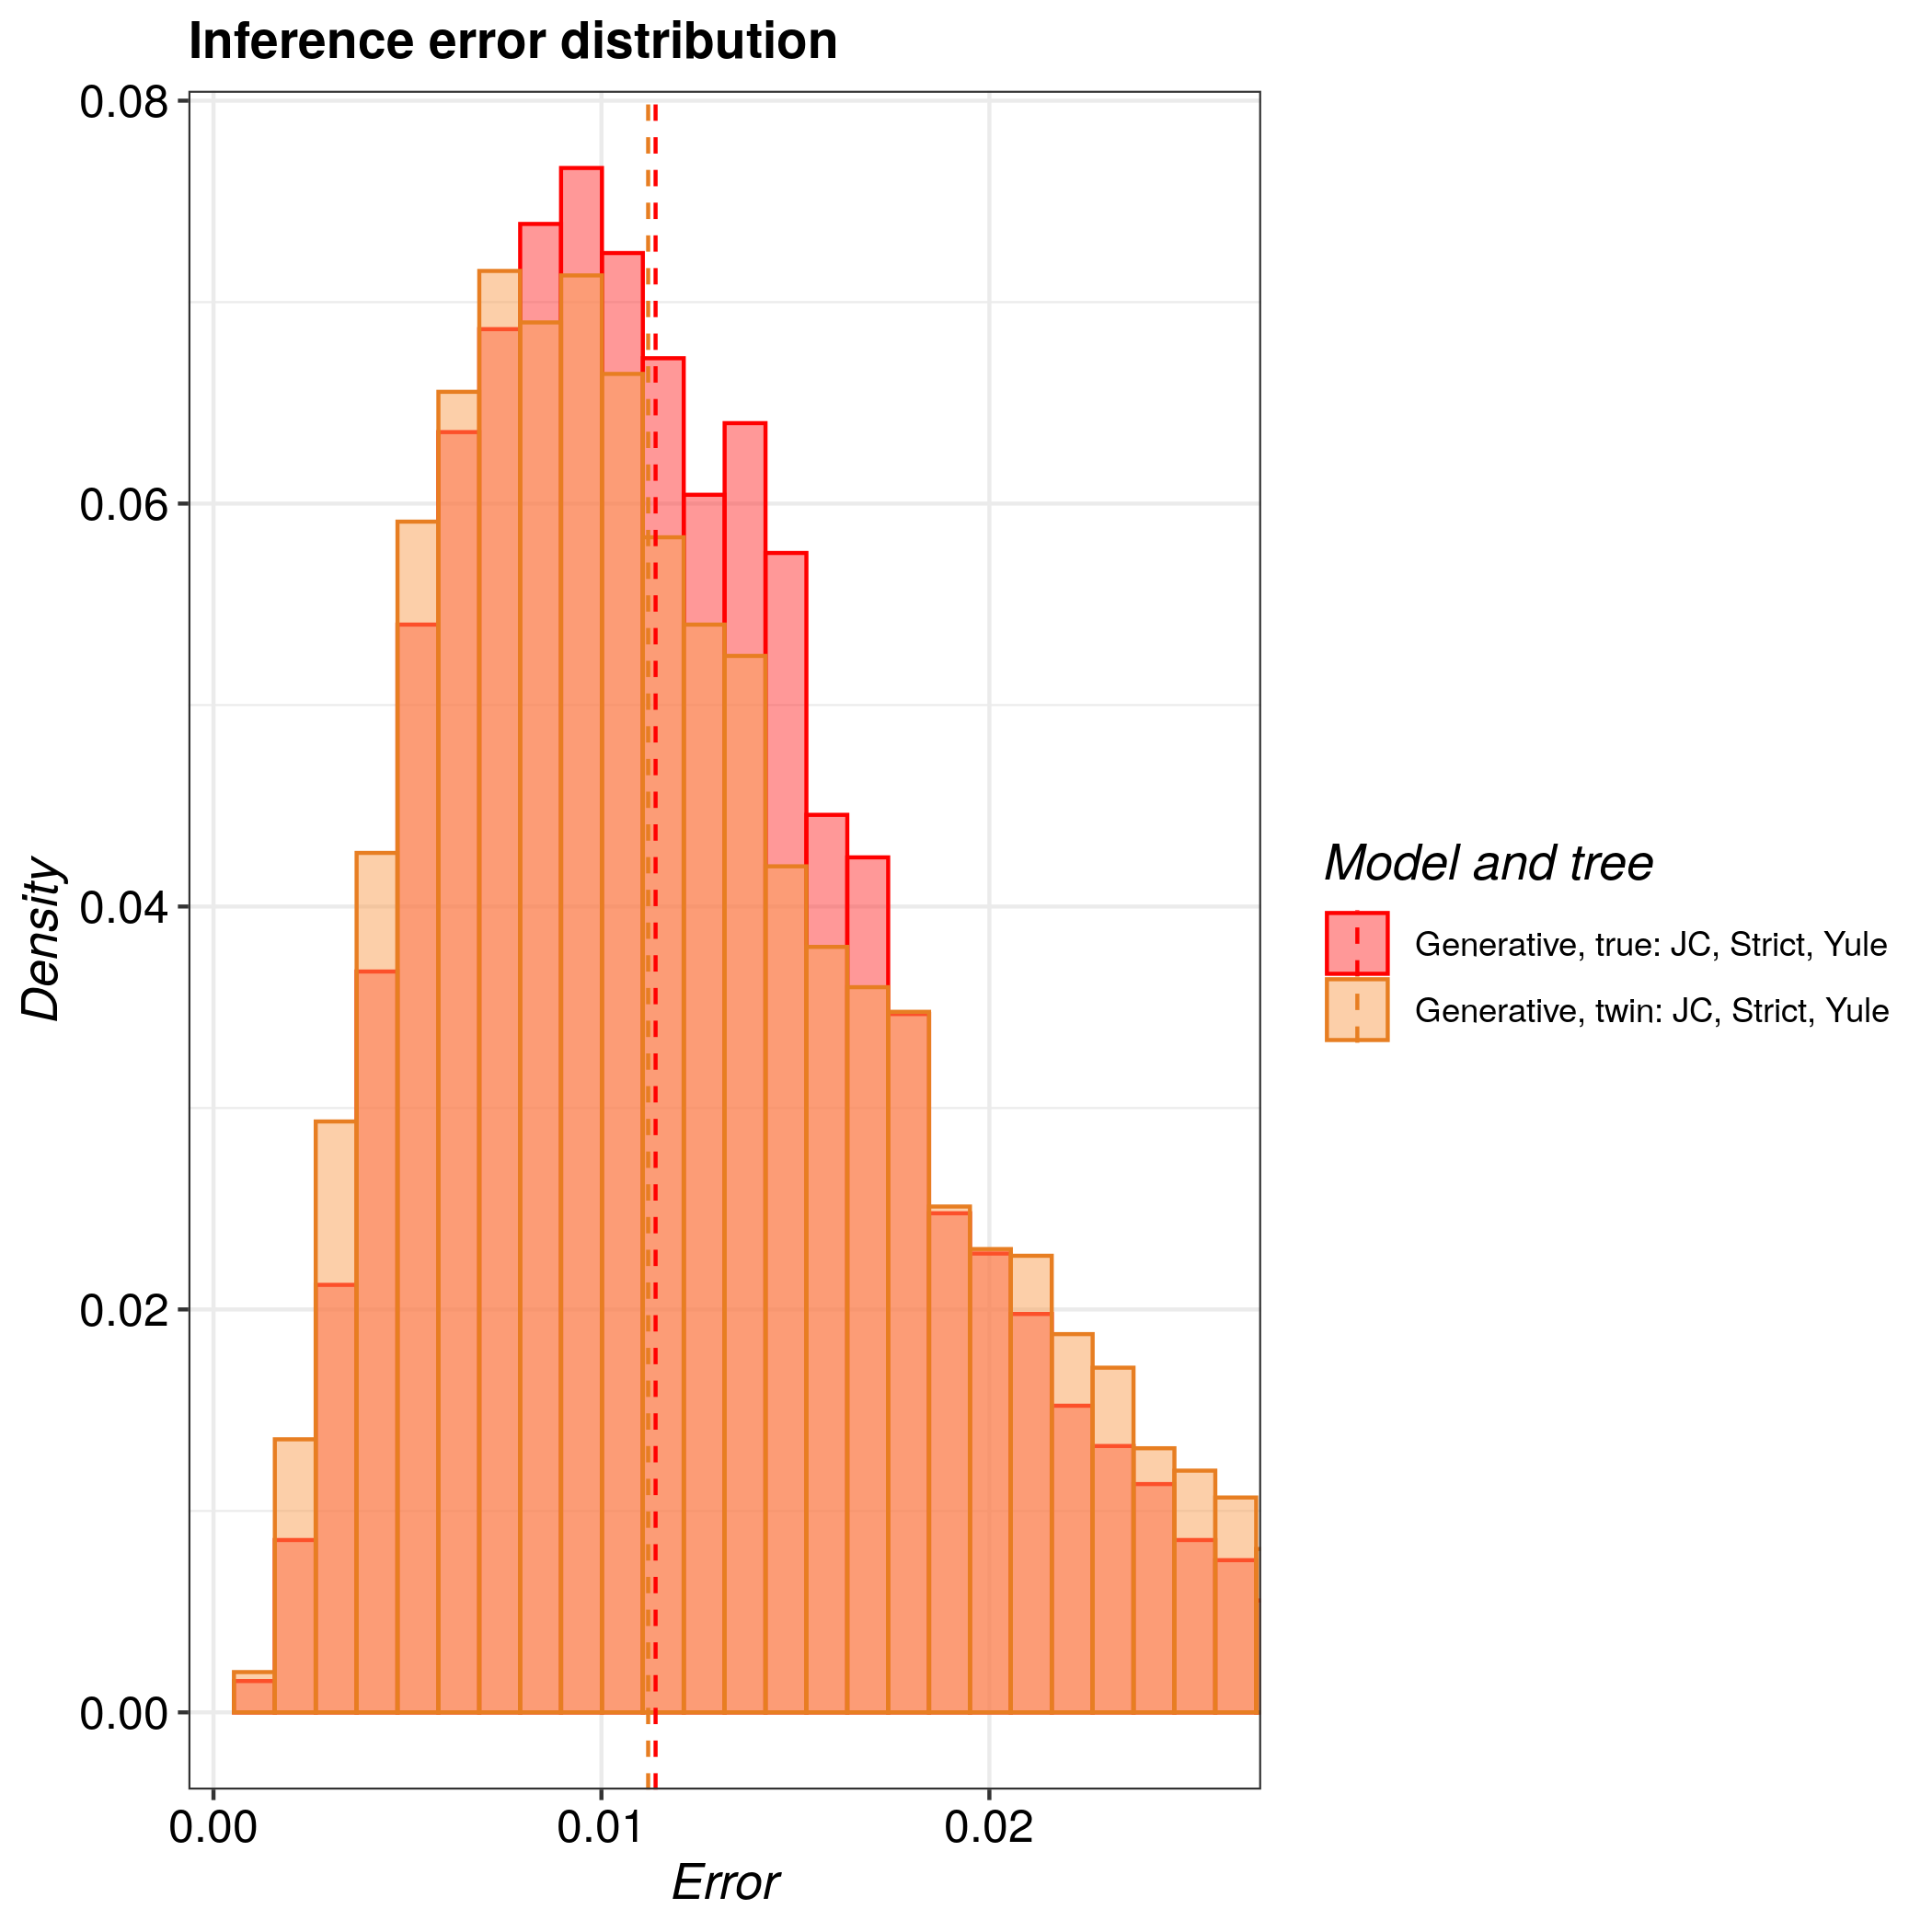
\includegraphics[width=\textwidth]{pirouette_example_24/example_24_316/errors.png}
  \caption{Per-nucleotide mutation rate of 0.05}
\end{figure}

\begin{figure}[H]
  \includegraphics[width=\textwidth]{pirouette_example_24/example_24_317/errors.png}
  \caption{Per-nucleotide mutation rate of 0.1}
\end{figure}

\begin{figure}[H]
  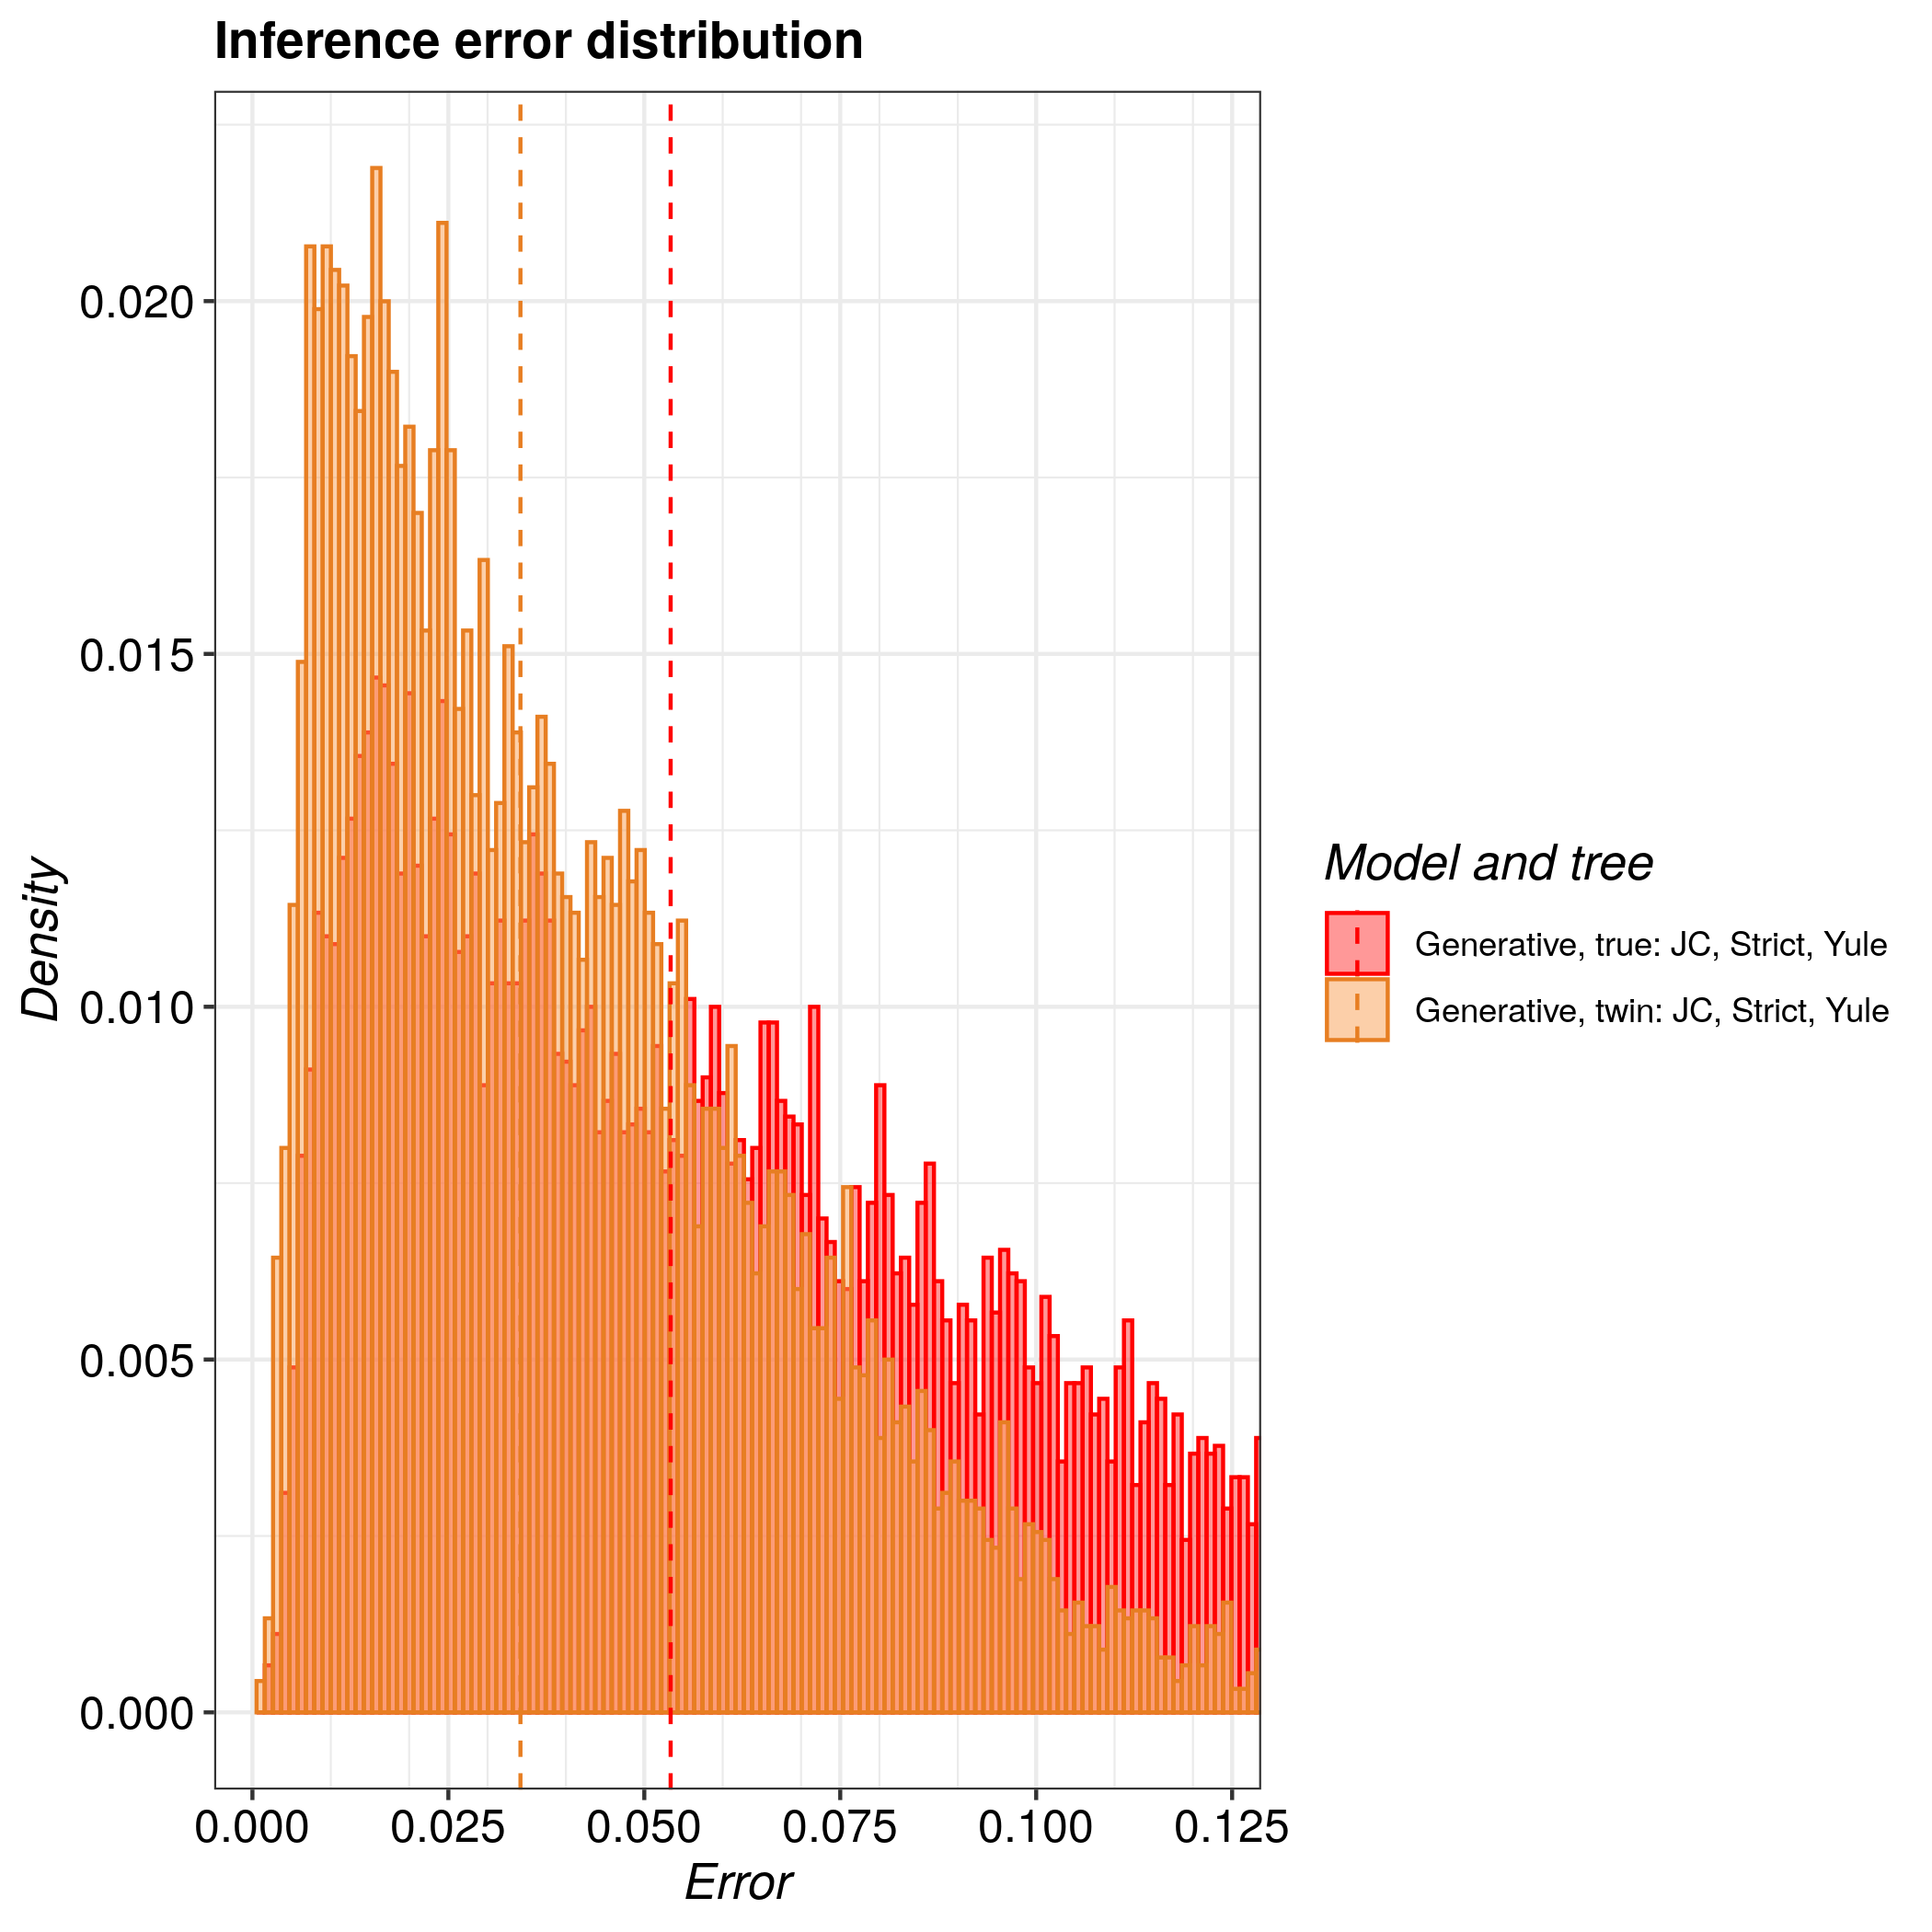
\includegraphics[width=\textwidth]{pirouette_example_24/example_24_318/errors.png}
  \caption{Per-nucleotide mutation rate of 0.2}
\end{figure}

\begin{figure}[H]
  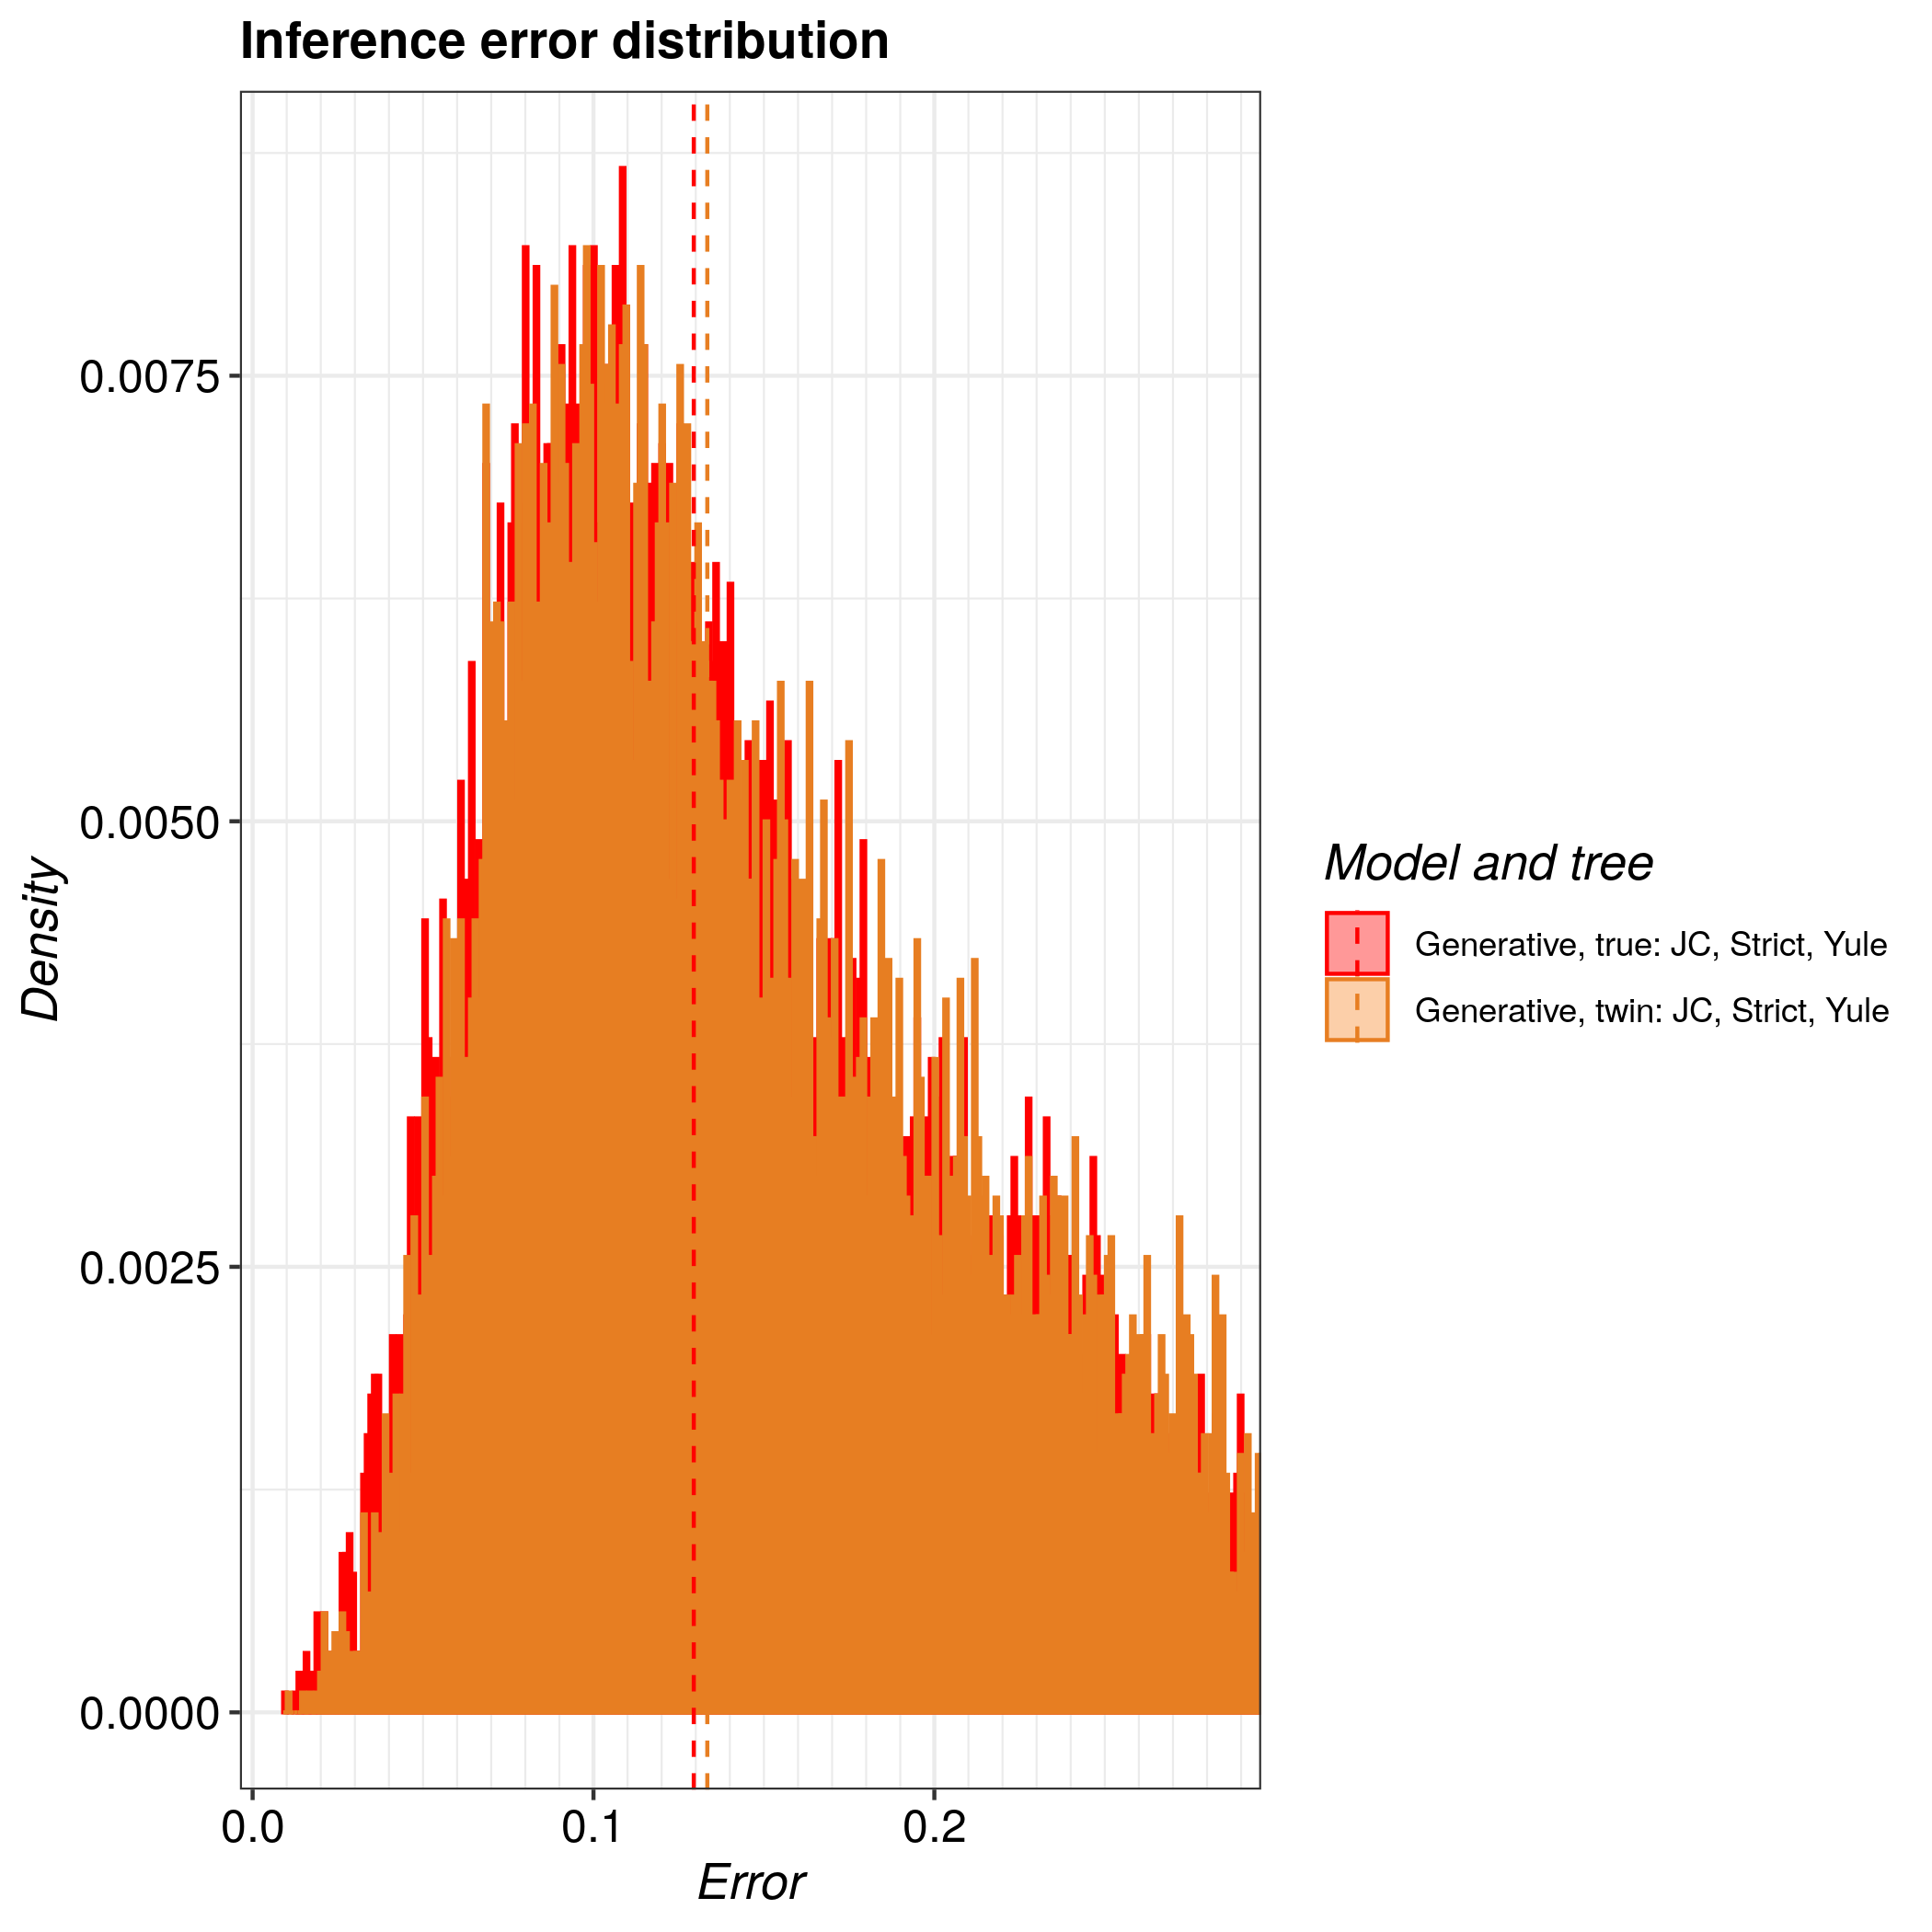
\includegraphics[width=\textwidth]{pirouette_example_24/example_24_319/errors.png}
  \caption{Per-nucleotide mutation rate of 0.4}
\end{figure}

\begin{figure}[H]
  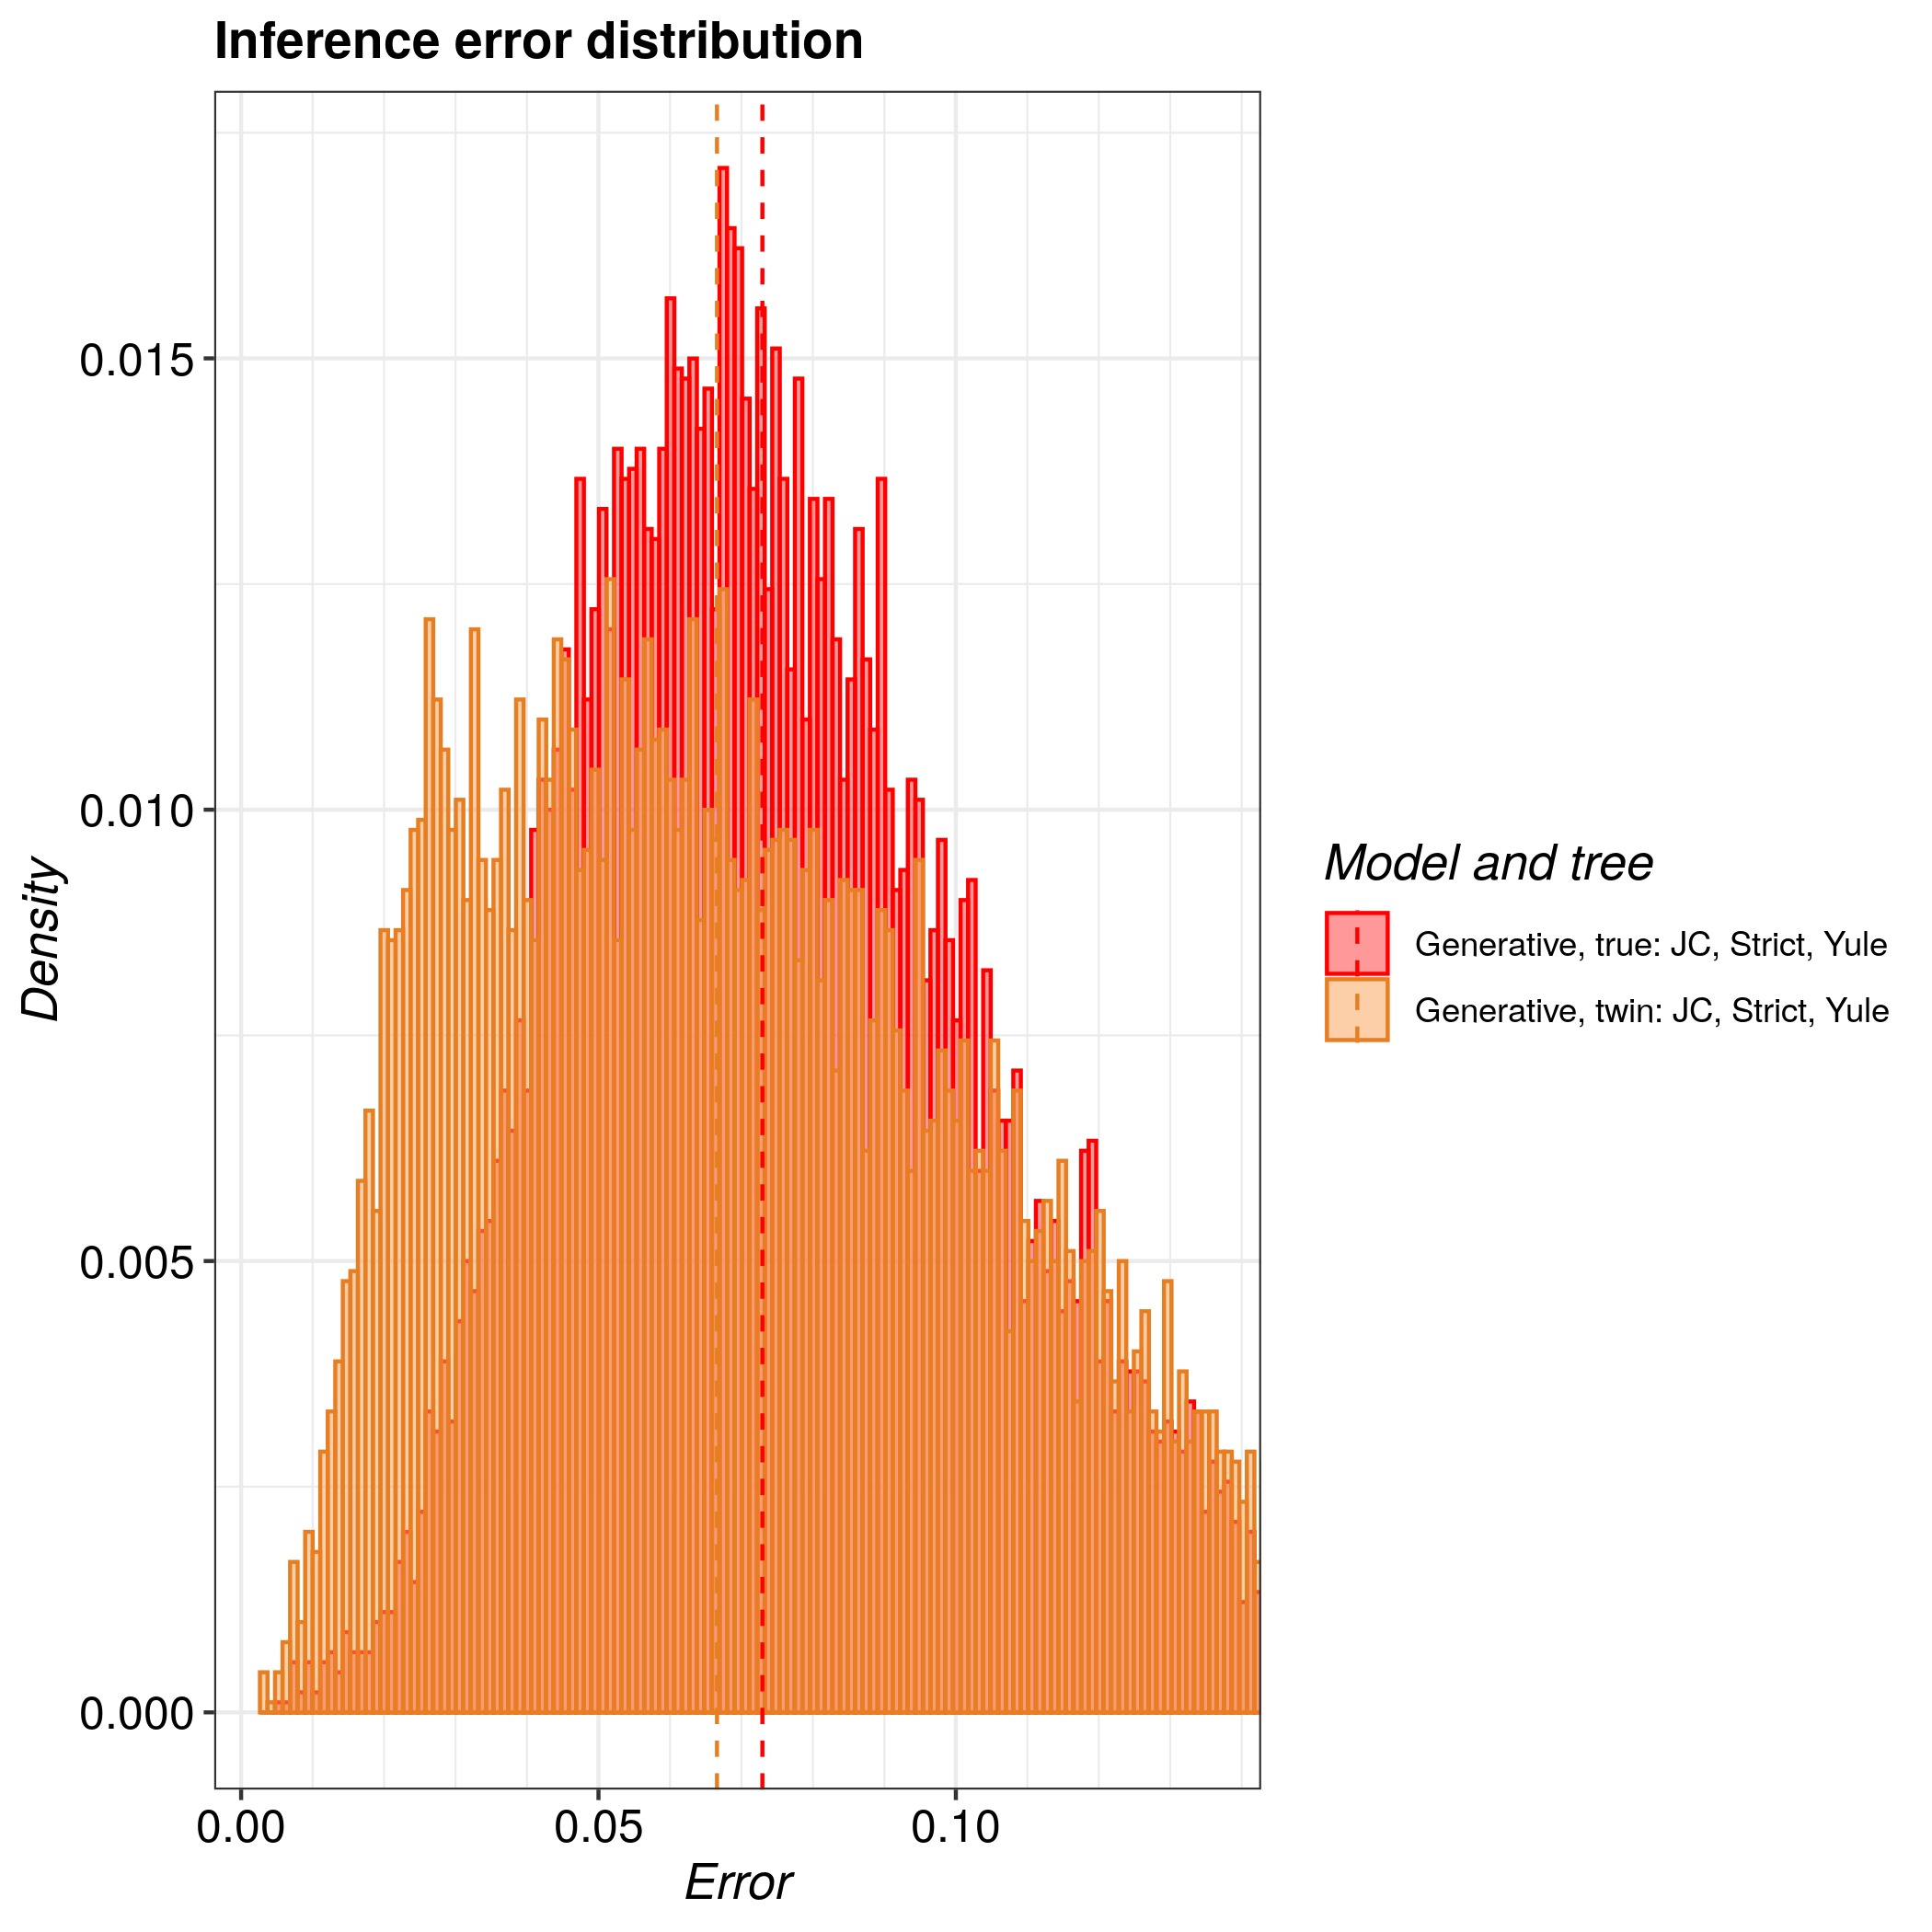
\includegraphics[width=\textwidth]{pirouette_example_24/example_24_320/errors.png}
  \caption{Per-nucleotide mutation rate of 0.8}
\end{figure}

